% 高一87_五十四中学_10月月考.tex
%   —— 高一上数学“2026-2027 年五十四中学高一上 10 月月考”（讲评版）
% 试卷版：xelatex 高一87_五十四中学_10月月考.tex
% 答案版：xelatex "\def\isanswer{1}% 高一87_五十四中学_10月月考.tex
%   —— 高一上数学“2026-2027 年五十四中学高一上 10 月月考”（讲评版）
% 试卷版：xelatex 高一87_五十四中学_10月月考.tex
% 答案版：xelatex "\def\isanswer{1}% 高一87_五十四中学_10月月考.tex
%   —— 高一上数学“2026-2027 年五十四中学高一上 10 月月考”（讲评版）
% 试卷版：xelatex 高一87_五十四中学_10月月考.tex
% 答案版：xelatex "\def\isanswer{1}% 高一87_五十四中学_10月月考.tex
%   —— 高一上数学“2026-2027 年五十四中学高一上 10 月月考”（讲评版）
% 试卷版：xelatex 高一87_五十四中学_10月月考.tex
% 答案版：xelatex "\def\isanswer{1}\input{高一87_五十四中学_10月月考.tex}"
% 紧凑版：xelatex "\def\iscompact{1}\input{高一87_五十四中学_10月月考.tex}"
%
% 原始材料：微信公众号“魔都数学加油站”文章，连载“27学年高一87”；
% 原文标题“27学年高一87——2026-2027年上海市五十四中学高一上10月月考”；
% 原文链接：https://mp.weixin.qq.com/s/pqPpSGQt0AhydcpaB8uEkQ。
% 页面标注发布时间 2026-10-27 17:43（上海）。
% 正文为 7 张 PNG 页（`原图/高一87_五十四中学_10月月考/01..07.png`），
% 尺寸混排（第 1、2 页为 4762×6735，第 3—7 页为 2560×3620），均按页序读取。
%
% 篇幅与题号：原卷自第 3 题起编号（第 1、2 题不在原文内）。填空题 3—12（10 题）、
% 选择题 13—16（4 题）、解答题 17—21（5 题），共 19 题。
%
% 讲评版：第 3、5、6 题只印【答案】（“$x\leqslant1$ 且 $y\leqslant1$”“$\{(2,6),(6,2)\}$”
% “$(-1,3]$”），本稿只给 \ans{}；其余 16 题印【解析】，其中选择题答案在解析末句
% “故选 A／B／D／B”。第 14 题题干带一幅韦恩图（裁自第 3 页原图、去粉色水印后转灰度），
% 三版都出。
%
% 副标题：原卷未印副标题。本稿按内容标作“集合与常用逻辑用语、不等式”。
%
% 原卷笔误/存疑（均照录未改，正文对应处另有 % 注）：
%   ① 第 19 题 (1) 解析作“所以 $A\cup b=(-\infty,3)\cup(5m+\infty)$”，两处均系排印错：
%      按上下文应为“$A\cup B=(-\infty,3)\cup(5,+\infty)$”（同页下一行 $\overline A\cap B$
%      的端点 $5$、$+\infty$ 也印证这一点）。原卷印作 $b$ 与 $5m+\infty$，照录未改。
%
% 与原卷的排版差异：
%   ① 原卷每题下直接印【答案】/【解析】，本稿按全稿惯例将答案与解析置于答案版；
%   ② 原卷未印副标题，本稿补出；填空横线统一排 \blankline[4.4em]；
%   ③ 原卷数集记号排斜体 $R$、$Z$、$N$，本稿按全稿惯例改用 $\R$、$\Z$、$\N$；
%   ④ 第 17—21 题的子问用行内“（1）（2）（3）”段，解析中的子问标号用 \stepm；
%   ⑤ 解答题按惯例加 \ansspace；选择题括号排 \mbox{（\quad）}。
%
% 行数核对：逐题数 \step/\stepm 条数，合计 86 条（Q4：1；Q7：4；Q8：2；Q9：2；Q10：3；
% Q11：9；Q12：3；Q13：2；Q14：3；Q15：5；Q16：9；Q17：6；Q18：3；Q19：7；Q20：13；
% Q21：14）；第 3、5、6 题只印【答案】，提 \ans{}，不计入 \step 账。原卷解析的换行
% 按语意合并，未逐行强拆。
%
\documentclass[a4paper,11pt]{article}
\usepackage{common}

\begin{document}

\examtitlest[7]{2026--2027 年五十四中学高一上 10 月月考}{集合与常用逻辑用语、不等式}

\bigsec{一、填空题}

\begin{enumerate}
\setcounter{enumi}{2}

\item “$x>1$ 或 $y>1$”的否定形式为\blankline[4.4em].

\ifanswer
\ans{$x\leqslant1$ 且 $y\leqslant1$}
\fi

\item 已知 $1<a<2$，$-3<b<3$，则 $a+b$ 的取值范围是\blankline[4.4em].

\ifanswer
\solbegin
\step{由不等式的可加性得 $-2<a+b<5$，故 $a+b$ 的取值范围是 $(-2,5)$.}
\solend
\fi

\item 方程组 $\begin{cases}x+y=8\\ xy=12\end{cases}$ 的解集为\blankline[4.4em].

\ifanswer
\ans{$\{(2,6),(6,2)\}$}
\fi

\item 不等式 $\dfrac{x-3}{x+1}\leqslant0$ 解集为\blankline[4.4em].

\ifanswer
\ans{$(-1,3]$}
\fi

\item 已知集合 $A=\{x\mid y=\sqrt{x+1}\}$，$B=\{y\mid y=x^2+5\}$，则 $A\cup B=\blankline[4.4em]$.

\ifanswer
\solbegin
\step{对于函数 $y=\sqrt{x+1}$，则 $x+1\geqslant0$，解得 $x\geqslant-1$，}
\step{所以 $A=\{x\mid y=\sqrt{x+1}\}=\{x\mid x\geqslant-1\}$，}
\step{因为 $x^2\geqslant0$，所以 $y=x^2+5\geqslant5$，所以 $B=\{y\mid y=x^2+5\}=\{y\mid y\geqslant5\}$，}
\step{所以 $A\cup B=\{x\mid x\geqslant-1\}$.}
\solend
\fi

\item 已知关于 $x$ 的不等式 $\lvert x+a\rvert<b$ 的解集为 $\{x\mid2<x<4\}$，则 $a+b$ 的值是\blankline[4.4em].

\ifanswer
\solbegin
\step{由 $\lvert x+a\rvert<b$，得 $-b-a<x<b-a$，则 $\begin{cases}-b-a=2\\ b-a=4\end{cases}$，解得 $a=-3$，$b=1$，}
\step{所以 $a+b=-2$.}
\solend
\fi

\item 已知一元二次方程 $x^2-2mx+m-1=0$ 的两实根为 $x_1,x_2$，且 $x_1^2+x_2^2=4$，则实数 $m$ 的值
是\blankline[4.4em].

\ifanswer
\solbegin
\step{由题意得 $x_1+x_2=2m$，$x_1x_2=m-1$，}
\step{所以 $x_1^2+x_2^2=(x_1+x_2)^2-2x_1x_2=4m^2-2m+2=4$，解得 $m=1$ 或 $m=-\dfrac12$.}
\solend
\fi

\item 已知集合 $A=\{x\mid x^2-x-6=0\}$，$B=\{y\mid ay-1=0\}$，若 $A\cap B=B$，则实数
$a=\blankline[4.4em]$.

\ifanswer
\solbegin
\step{$A=\{-2,3\}$，由 $A\cap B=B$，得 $B\subseteq A$，而 $B=\{y\mid ay-1=0\}$，}
\step{则当 $B=\varnothing$ 时，$a=0$；当 $B=\{-2\}$ 时，$-2a-1=0$，解得 $a=-\dfrac12$；}
\step{当 $B=\{3\}$ 时，$3a-1=0$，解得 $a=\dfrac13$，所以实数 $a$ 的值为 $-\dfrac12$ 或 $0$ 或 $\dfrac13$.}
\solend
\fi

\item 已知集合 $A=\{x\mid(m-1)x^2+(m-1)x+2\leqslant0,x\in\R\}$，$B=\left\{x\left|\dfrac{2x-1}{x^2+x+1}>1,x\in\R\right.\right\}$，
且 $A\cap B=A$，则实数 $m$ 的取值范围是\blankline[4.4em].

\ifanswer
\solbegin
\step{因为 $\dfrac{2x-1}{x^2+x+1}>1$，所以 $x^2-x+2<0$，显然不等式无解，}
\step{所以 $B=\left\{x\left|\dfrac{2x-1}{x^2+x+1}>1,x\in\R\right.\right\}=\varnothing$，而 $A\cap B=A$，则 $A=\varnothing$，}
\step{①当 $m=1$ 时，$2\leqslant0$ 不成立，此时 $A=\varnothing$，}
\step{②当 $m<1$ 时，$m-1<0$，函数 $y=(m-1)x^2+(m-1)x+2$，开口向下，}
\step{不等式 $(m-1)x^2+(m-1)x+2\leqslant0$ 有解，$A\neq\varnothing$，}
\step{③当 $m>1$ 时，函数 $y=(m-1)x^2+(m-1)x+2$，开口向上，}
\step{若不等式 $(m-1)x^2+(m-1)x+2\leqslant0$ 无解，}
\step{只需 $\Delta=(m-1)^2-8(m-1)<0$，解得 $1<m<9$，}
\step{综上，$m$ 的取值范围是 $[1,9]$.}
\solend
\fi

\item 设 $A$ 是整数集的一个非空子集，对于 $k\in A$，如果 $k-1\notin A$ 且 $k+1\notin A$，那么 $k$ 是 $A$
的一个“孤立元”. 给定 $S=\{1,2,3,4,5,6,7,8\}$，由 $S$ 的 $3$ 个元素构成的所有集合中，不含
“孤立元”的集合共有\blankline[3.6em]个.

\ifanswer
\solbegin
\step{由题意得，“孤立元”即为在集合中无与之相邻的元素，}
\step{满足条件的集合有 $\{1,2,3\},\{2,3,4\},\{3,4,5\},\{4,5,6\},\{5,6,7\},\{6,7,8\}$，}
\step{共 $6$ 个集合.}
\solend
\fi

\end{enumerate}

\bigsec{二、选择题}

\begin{enumerate}
\setcounter{enumi}{12}

\item “$m=2$”是“$m^2=4$”的\mbox{（\quad）}条件.

\keepwithprev
A. 充分非必要条件\qquad B. 必要非充分条件

C. 充要条件\qquad D. 既非充分又非必要条件

\ifanswer
\solbegin
\step{由 $m^2=4$，解得 $m=\pm2$，故“$m=2$”是“$m^2=4$”的充分不必要条件，}
\step{故选 $A$.}
\solend
\fi

\item 已知全集 $U=\R$，集合 $M=\{x\mid\lvert x-1\rvert\leqslant2\}$ 和 $N=\{x\mid x=2k-1,k\in\Z\}$ 的关系
的韦恩（$Venn$）图如图所示，则阴影部分所示的集合的元素共有\mbox{（\quad）}

\begin{center}
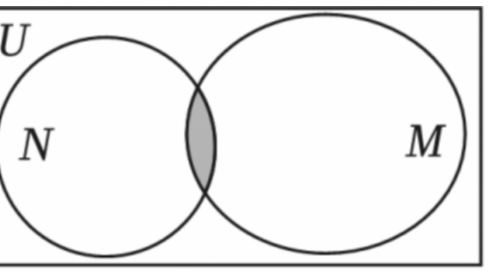
\includegraphics[width=0.30\textwidth]{figures/gao87_q14_venn.png}
\end{center}

\keepwithprev
A. $3$ 个\qquad B. $2$ 个\qquad C. $1$ 个\qquad D. 无穷多个

\ifanswer
\solbegin
\step{阴影部分所示的集合为 $M\cap N$，}
\step{$M=\{x\mid-1\leqslant x\leqslant3\}$，在此范围内的奇数有 $1$ 和 $3$，}
\step{所以集合 $M\cap N=\{1,3\}$ 共有 $2$ 个元素，故选 $B$.}
\solend
\fi

\item 已知实数 $a,b,c$ 满足 $a>b$，则下列不等式成立的是\mbox{（\quad）}

\keepwithprev
A. $-\dfrac1a<\dfrac1b$\qquad B. $a^2>b^2$\qquad C. $a\lvert c\rvert>b\lvert c\rvert$\qquad D. $\dfrac a{c^2+1}>\dfrac b{c^2+1}$

\ifanswer
\solbegin
\step{若 $a=1,b=-1$，则 $-1=-\dfrac1a=\dfrac1b=1$，$a^2=b^2=1$，则 AB 错误；}
\step{若 $a>b,c=0$，则 $a\lvert c\rvert=b\lvert c\rvert=0$，则 C 错误；}
\step{因为 $c^2+1\geqslant1$，所以 $0<\dfrac1{c^2+1}\leqslant1$，又 $a>b$，所以 $\dfrac a{c^2+1}>\dfrac b{c^2+1}$，}
\step{则 D 正确.}
\step{故选 $D$.}
\solend
\fi

\item 设集合 $P_1=\{x\mid x^2+ax+1>0\}$，$P_2=\{x\mid x^2+ax+2>0\}$，$Q_1=\{x\mid x^2+x+b>0\}$，
$Q_2=\{x\mid x^2+2x+b>0\}$，其中 $a$、$b\in\R$，下列说法中正确的是\mbox{（\quad）}

\keepwithprev
A. 对任意 $a$，$P_1$ 是 $P_2$ 的子集，对任意 $b$，$Q_1$ 不是 $Q_2$ 的子集

B. 对任意 $a$，$P_1$ 是 $P_2$ 的子集，存在 $b$，使得 $Q_1$ 是 $Q_2$ 的子集

C. 存在 $a$，使得 $P_1$ 不是 $P_2$ 的子集，对任意 $b$，$Q_1$ 不是 $Q_2$ 的子集

D. 存在 $a$，使得 $P_1$ 不是 $P_2$ 的子集，存在 $b$，使得 $Q_1$ 是 $Q_2$ 的子集

\ifanswer
\solbegin
\step{对于集合 $P_1=\{x\mid x^2+ax+1>0\}$，$P_2=\{x\mid x^2+ax+2>0\}$，}
\step{得当 $m\in P_1$ 时，即 $m^2+am+1>0$，得 $m^2+am+2>0$，}
\step{即有 $m\in P_2$，得对任意 $a$，$P_1$ 是 $P_2$ 的子集，}
\step{对于集合 $Q_1=\{x\mid x^2+x+b>0\}$，$Q_2=\{x\mid x^2+2x+b>0\}$，}
\step{当 $b=6$ 时，$Q_1=\{x\mid x^2+x+6>0\}=\R$，$Q_2=\{x\mid x^2+2x+6>0\}=\R$，}
\step{得 $Q_1$ 是 $Q_2$ 的子集，}
\step{当 $b=1$ 时，$Q_1=\{x\mid x^2+x+1>0\}=\R$，}
\step{$Q_2=\{x\mid x^2+2x+1>0\}=\{x\mid x\neq-1\}$，得 $Q_1$ 不是 $Q_2$ 的子集，}
\step{所以存在 $b$，使得 $Q_1$ 是 $Q_2$ 的子集，故选 $B$.}
\solend
\fi

\end{enumerate}

\bigsec{三、解答题}

\begin{enumerate}
\setcounter{enumi}{16}

\item 设 $m$ 为实数，求关于 $x$ 与 $y$ 的二元一次方程组 $\begin{cases}y=x+m\\ mx-y=4\end{cases}$ 的解集.

\ansspace*[8]

\ifanswer
\solbegin
\step{消去 $y$ 得 $(m-1)x=m+4$，}
\step{当 $m-1=0$，即 $m=1$ 时，$0=5$ 不成立，则 $x$ 无解，原方程组的解集为 $\varnothing$；}
\step{当 $m-1\neq0$，即 $m\neq1$ 时，则 $x=\dfrac{m+4}{m-1}$，$y=\dfrac{m+4}{m-1}+m=\dfrac{m^2+4}{m-1}$，}
\step{原方程组的解集为 $\left\{\left(\dfrac{m+4}{m-1},\dfrac{m^2+4}{m-1}\right)\right\}$.}
\step{综上所述，当 $m=1$ 时，方程组的解集为 $\varnothing$；}
\step{当 $m\neq1$ 时，方程组的解集为 $\left\{\left(\dfrac{m+4}{m-1},\dfrac{m^2+4}{m-1}\right)\right\}$.}
\solend
\fi

\item 设 $x<y<0$，试比较 $(x^2+y^2)(x-y)$ 与 $(x^2-y^2)(x+y)$ 的大小.

\ansspace*[9]

\ifanswer
\solbegin
\step{$(x^2+y^2)(x-y)-(x^2-y^2)(x+y)=(x-y)[x^2+y^2-(x+y)^2]=-2xy(x-y)$，}
\step{因为 $x<y<0$，所以 $xy>0$，$x-y<0$，所以 $-2xy(x-y)>0$，}
\step{即 $(x^2+y^2)(x-y)>(x^2-y^2)(x+y)$.}
\solend
\fi

\item 已知全集 $U=\R$，集合 $A=\left\{x\left|\dfrac{2+x}{3-x}>0\right.\right\}$，集合 $B=\{x\mid\lvert x-2\rvert>3\}$.

（1）求 $A\cup B$、$\overline A\cap B$.

（2）若集合 $C=\{x\mid x\leqslant a\}$，且 $A\cap C=A$，求实数 $a$ 的范围.

\ansspace*[10]

\ifanswer
\solbegin
\stepm{（1）}{由 $\lvert x-2\rvert>3$ 得 $x-2>3$ 或 $x-2<-3$，即 $x<-1$ 或 $x>5$，}
\step{所以 $B=(-\infty,-1)\cup(5,+\infty)$，}
\step{$A=\left\{x\left|\dfrac{2+x}{3-x}>0\right.\right\}=\{x\mid(2+x)(3-x)>0\}=(-2,3)$，}
\step{所以 $A\cup b=(-\infty,3)\cup(5m+\infty)$，}
\step{$\overline A=(-\infty,-2]\cup[3,+\infty)$，$\overline A\cap B=(-\infty,-2]\cup(5,+\infty)$.}
\stepm{（2）}{因为 $A\cap C=A$，所以 $A\subseteq C$，}
\step{因为 $A=(-2,3)$，所以实数 $a$ 的取值范围为 $\{a\mid a\geqslant3\}$.}
\solend
\fi

\item 已知函数 $f(x)=ax^2+4x+b\,(a<0,a,b\in\R)$，设关于 $x$ 的方程 $f(x)=0$ 的两实根为 $x_1$、
$x_2$，方程 $f(x)=x$ 的两实根为 $\alpha,\beta$.

（1）不等式 $f(x)<0$ 的解集是 $(-\infty,-3)\cup(5,+\infty)$，求不等式 $bx^2-ax-4<0$ 的解集；

（2）若 $a,b$ 均为负整数，且 $\lvert\alpha-\beta\rvert=1$，求 $f(x)$ 的解析式.

\ansspace*[12]

\ifanswer
\solbegin
\stepm{（1）}{$ax^2+4x+b<0$ 的解集为 $(-\infty,-3)\cup(5,+\infty)$，}
\step{所以 $-3,5$ 是方程 $ax^2+4x+b=0$ 的两根，所以 $\begin{cases}-3+5=-\dfrac4a\\ -3\times5=\dfrac ba\end{cases}\Rightarrow\begin{cases}a=-2\\ b=30\end{cases}$，}
\step{所以 $bx^2-ax-4<0$ 为 $30x^2+2x-4<0\Rightarrow15x^2+x-2<0$，}
\step{所以 $(3x-1)(5x+2)<0\Rightarrow-\dfrac25<x<\dfrac13$，}
\step{所以所求不等式的解集为 $\left\{x\left|-\dfrac25<x<\dfrac13\right.\right\}$.}
\stepm{（2）}{由题意得 $f(x)=ax^2+4x+b\,(a<0,a,b\in\R)$ 有两个不等实根为 $\alpha$、$\beta$，}
\step{所以 $\Delta=9-4ab>0$，$\alpha+\beta=-\dfrac3a$，$\alpha\beta=\dfrac ba$.}
\step{由 $\lvert\alpha-\beta\rvert=1$ 得 $(\alpha-\beta)^2=1$，即 $(\alpha+\beta)^2-4\alpha\beta=\dfrac9{a^2}-\dfrac{4b}a=1$，}
\step{所以 $9-4ab=a^2$，即 $a^2+4ab=9\,(a<0,a,b\in\R)$.}
\step{因为 $a,b$ 均为负整数，}
\step{所以 $\begin{cases}a=-1\\ a+4b=-9\end{cases}$ 或 $\begin{cases}a=-9\\ a+4b=-1\end{cases}$ 或 $\begin{cases}a=-3\\ a+4b=-3\end{cases}$，}
\step{显然后两种情况不合题意，应舍去，从而有 $\begin{cases}a=-1\\ a+4b=-9\end{cases}$，解得 $a=-1$，$b=-2$.}
\step{故所求函数解析式为 $f(x)=-x^2+4x-2$.}
\solend
\fi

\item 已知集合 $A=\{x\mid x=m^2+n^2,m\in\Z,n\in\Z\}$.

（1）判断 $2,5,25$ 是否属于集合 $A$；

（2）若正整数 $y$ 能表示为某个整数的平方，$z\in A$，证明：$yz\in A$；

（3）若集合 $B=\{x\mid x=4k+3,k\in\Z\}$，证明：$A\cap B=\varnothing$.

\ansspace*[14]

\ifanswer
\solbegin
\stepm{（1）}{由 $2=1^2+1^2$，$5=1^2+2^2$，$25=3^2+4^2$ 得 $2,5,25$ 属于集合 $A$；}
\stepm{（2）}{设 $y=a^2\,(a\in\Z)$，由 $z\in A$，设 $z=b^2+c^2\,(b\in\Z,c\in\Z)$，}
\step{则 $yz=a^2(b^2+c^2)=(ab)^2+(ac)^2$，}
\step{因为 $a\in\Z$，$b\in\Z$，$c\in\Z$，所以 $ab\in\Z$，$ac\in\Z$，所以 $yz\in A$；}
\stepm{（3）}{①当 $m$、$n$ 都为偶数时，设 $m=2k_1\,(k_1\in\Z)$，$n=2k_2\,(k_2\in\Z)$，}
\step{则 $x=m^2+n^2=4k_1^2+4k_2^2=4(k_1^2+k_2^2)$，此时 $x$ 为 $4$ 的倍数，}
\step{因为偶数 $\notin B$，所以 $A\cap B=\varnothing$；}
\step{②当 $m$、$n$ 都为奇数时，设 $m=2k_1+1\,(k_1\in\Z)$，$n=2k_2+1\,(k_2\in\Z)$，}
\step{则 $x=m^2+n^2=(2k_1+1)^2+(2k_2+1)^2=4(k_1^2+k_2^2+k_1+k_2)+2$，}
\step{此时 $x$ 为 $2$ 的倍数，因为偶数 $\notin B$，所以 $A\cap B=\varnothing$；}
\step{③当 $m$、$n$ 一奇一偶时，设 $m=2k_1+1\,(k_1\in\Z)$，$n=2k_2\,(k_2\in\Z)$，}
\step{则 $x=m^2+n^2=(2k_1+1)^2+(2k_2)^2=4(k_1^2+k_2^2+k_1)+1$，}
\step{此时 $x$ 被 $4$ 除余 $1$，而 $B$ 中元素被 $4$ 除余 $3$，此时 $A\cap B=\varnothing$.}
\step{综上，$A\cap B=\varnothing$.}
\solend
\fi

\end{enumerate}

\end{document}
"
% 紧凑版：xelatex "\def\iscompact{1}% 高一87_五十四中学_10月月考.tex
%   —— 高一上数学“2026-2027 年五十四中学高一上 10 月月考”（讲评版）
% 试卷版：xelatex 高一87_五十四中学_10月月考.tex
% 答案版：xelatex "\def\isanswer{1}\input{高一87_五十四中学_10月月考.tex}"
% 紧凑版：xelatex "\def\iscompact{1}\input{高一87_五十四中学_10月月考.tex}"
%
% 原始材料：微信公众号“魔都数学加油站”文章，连载“27学年高一87”；
% 原文标题“27学年高一87——2026-2027年上海市五十四中学高一上10月月考”；
% 原文链接：https://mp.weixin.qq.com/s/pqPpSGQt0AhydcpaB8uEkQ。
% 页面标注发布时间 2026-10-27 17:43（上海）。
% 正文为 7 张 PNG 页（`原图/高一87_五十四中学_10月月考/01..07.png`），
% 尺寸混排（第 1、2 页为 4762×6735，第 3—7 页为 2560×3620），均按页序读取。
%
% 篇幅与题号：原卷自第 3 题起编号（第 1、2 题不在原文内）。填空题 3—12（10 题）、
% 选择题 13—16（4 题）、解答题 17—21（5 题），共 19 题。
%
% 讲评版：第 3、5、6 题只印【答案】（“$x\leqslant1$ 且 $y\leqslant1$”“$\{(2,6),(6,2)\}$”
% “$(-1,3]$”），本稿只给 \ans{}；其余 16 题印【解析】，其中选择题答案在解析末句
% “故选 A／B／D／B”。第 14 题题干带一幅韦恩图（裁自第 3 页原图、去粉色水印后转灰度），
% 三版都出。
%
% 副标题：原卷未印副标题。本稿按内容标作“集合与常用逻辑用语、不等式”。
%
% 原卷笔误/存疑（均照录未改，正文对应处另有 % 注）：
%   ① 第 19 题 (1) 解析作“所以 $A\cup b=(-\infty,3)\cup(5m+\infty)$”，两处均系排印错：
%      按上下文应为“$A\cup B=(-\infty,3)\cup(5,+\infty)$”（同页下一行 $\overline A\cap B$
%      的端点 $5$、$+\infty$ 也印证这一点）。原卷印作 $b$ 与 $5m+\infty$，照录未改。
%
% 与原卷的排版差异：
%   ① 原卷每题下直接印【答案】/【解析】，本稿按全稿惯例将答案与解析置于答案版；
%   ② 原卷未印副标题，本稿补出；填空横线统一排 \blankline[4.4em]；
%   ③ 原卷数集记号排斜体 $R$、$Z$、$N$，本稿按全稿惯例改用 $\R$、$\Z$、$\N$；
%   ④ 第 17—21 题的子问用行内“（1）（2）（3）”段，解析中的子问标号用 \stepm；
%   ⑤ 解答题按惯例加 \ansspace；选择题括号排 \mbox{（\quad）}。
%
% 行数核对：逐题数 \step/\stepm 条数，合计 86 条（Q4：1；Q7：4；Q8：2；Q9：2；Q10：3；
% Q11：9；Q12：3；Q13：2；Q14：3；Q15：5；Q16：9；Q17：6；Q18：3；Q19：7；Q20：13；
% Q21：14）；第 3、5、6 题只印【答案】，提 \ans{}，不计入 \step 账。原卷解析的换行
% 按语意合并，未逐行强拆。
%
\documentclass[a4paper,11pt]{article}
\usepackage{common}

\begin{document}

\examtitlest[7]{2026--2027 年五十四中学高一上 10 月月考}{集合与常用逻辑用语、不等式}

\bigsec{一、填空题}

\begin{enumerate}
\setcounter{enumi}{2}

\item “$x>1$ 或 $y>1$”的否定形式为\blankline[4.4em].

\ifanswer
\ans{$x\leqslant1$ 且 $y\leqslant1$}
\fi

\item 已知 $1<a<2$，$-3<b<3$，则 $a+b$ 的取值范围是\blankline[4.4em].

\ifanswer
\solbegin
\step{由不等式的可加性得 $-2<a+b<5$，故 $a+b$ 的取值范围是 $(-2,5)$.}
\solend
\fi

\item 方程组 $\begin{cases}x+y=8\\ xy=12\end{cases}$ 的解集为\blankline[4.4em].

\ifanswer
\ans{$\{(2,6),(6,2)\}$}
\fi

\item 不等式 $\dfrac{x-3}{x+1}\leqslant0$ 解集为\blankline[4.4em].

\ifanswer
\ans{$(-1,3]$}
\fi

\item 已知集合 $A=\{x\mid y=\sqrt{x+1}\}$，$B=\{y\mid y=x^2+5\}$，则 $A\cup B=\blankline[4.4em]$.

\ifanswer
\solbegin
\step{对于函数 $y=\sqrt{x+1}$，则 $x+1\geqslant0$，解得 $x\geqslant-1$，}
\step{所以 $A=\{x\mid y=\sqrt{x+1}\}=\{x\mid x\geqslant-1\}$，}
\step{因为 $x^2\geqslant0$，所以 $y=x^2+5\geqslant5$，所以 $B=\{y\mid y=x^2+5\}=\{y\mid y\geqslant5\}$，}
\step{所以 $A\cup B=\{x\mid x\geqslant-1\}$.}
\solend
\fi

\item 已知关于 $x$ 的不等式 $\lvert x+a\rvert<b$ 的解集为 $\{x\mid2<x<4\}$，则 $a+b$ 的值是\blankline[4.4em].

\ifanswer
\solbegin
\step{由 $\lvert x+a\rvert<b$，得 $-b-a<x<b-a$，则 $\begin{cases}-b-a=2\\ b-a=4\end{cases}$，解得 $a=-3$，$b=1$，}
\step{所以 $a+b=-2$.}
\solend
\fi

\item 已知一元二次方程 $x^2-2mx+m-1=0$ 的两实根为 $x_1,x_2$，且 $x_1^2+x_2^2=4$，则实数 $m$ 的值
是\blankline[4.4em].

\ifanswer
\solbegin
\step{由题意得 $x_1+x_2=2m$，$x_1x_2=m-1$，}
\step{所以 $x_1^2+x_2^2=(x_1+x_2)^2-2x_1x_2=4m^2-2m+2=4$，解得 $m=1$ 或 $m=-\dfrac12$.}
\solend
\fi

\item 已知集合 $A=\{x\mid x^2-x-6=0\}$，$B=\{y\mid ay-1=0\}$，若 $A\cap B=B$，则实数
$a=\blankline[4.4em]$.

\ifanswer
\solbegin
\step{$A=\{-2,3\}$，由 $A\cap B=B$，得 $B\subseteq A$，而 $B=\{y\mid ay-1=0\}$，}
\step{则当 $B=\varnothing$ 时，$a=0$；当 $B=\{-2\}$ 时，$-2a-1=0$，解得 $a=-\dfrac12$；}
\step{当 $B=\{3\}$ 时，$3a-1=0$，解得 $a=\dfrac13$，所以实数 $a$ 的值为 $-\dfrac12$ 或 $0$ 或 $\dfrac13$.}
\solend
\fi

\item 已知集合 $A=\{x\mid(m-1)x^2+(m-1)x+2\leqslant0,x\in\R\}$，$B=\left\{x\left|\dfrac{2x-1}{x^2+x+1}>1,x\in\R\right.\right\}$，
且 $A\cap B=A$，则实数 $m$ 的取值范围是\blankline[4.4em].

\ifanswer
\solbegin
\step{因为 $\dfrac{2x-1}{x^2+x+1}>1$，所以 $x^2-x+2<0$，显然不等式无解，}
\step{所以 $B=\left\{x\left|\dfrac{2x-1}{x^2+x+1}>1,x\in\R\right.\right\}=\varnothing$，而 $A\cap B=A$，则 $A=\varnothing$，}
\step{①当 $m=1$ 时，$2\leqslant0$ 不成立，此时 $A=\varnothing$，}
\step{②当 $m<1$ 时，$m-1<0$，函数 $y=(m-1)x^2+(m-1)x+2$，开口向下，}
\step{不等式 $(m-1)x^2+(m-1)x+2\leqslant0$ 有解，$A\neq\varnothing$，}
\step{③当 $m>1$ 时，函数 $y=(m-1)x^2+(m-1)x+2$，开口向上，}
\step{若不等式 $(m-1)x^2+(m-1)x+2\leqslant0$ 无解，}
\step{只需 $\Delta=(m-1)^2-8(m-1)<0$，解得 $1<m<9$，}
\step{综上，$m$ 的取值范围是 $[1,9]$.}
\solend
\fi

\item 设 $A$ 是整数集的一个非空子集，对于 $k\in A$，如果 $k-1\notin A$ 且 $k+1\notin A$，那么 $k$ 是 $A$
的一个“孤立元”. 给定 $S=\{1,2,3,4,5,6,7,8\}$，由 $S$ 的 $3$ 个元素构成的所有集合中，不含
“孤立元”的集合共有\blankline[3.6em]个.

\ifanswer
\solbegin
\step{由题意得，“孤立元”即为在集合中无与之相邻的元素，}
\step{满足条件的集合有 $\{1,2,3\},\{2,3,4\},\{3,4,5\},\{4,5,6\},\{5,6,7\},\{6,7,8\}$，}
\step{共 $6$ 个集合.}
\solend
\fi

\end{enumerate}

\bigsec{二、选择题}

\begin{enumerate}
\setcounter{enumi}{12}

\item “$m=2$”是“$m^2=4$”的\mbox{（\quad）}条件.

\keepwithprev
A. 充分非必要条件\qquad B. 必要非充分条件

C. 充要条件\qquad D. 既非充分又非必要条件

\ifanswer
\solbegin
\step{由 $m^2=4$，解得 $m=\pm2$，故“$m=2$”是“$m^2=4$”的充分不必要条件，}
\step{故选 $A$.}
\solend
\fi

\item 已知全集 $U=\R$，集合 $M=\{x\mid\lvert x-1\rvert\leqslant2\}$ 和 $N=\{x\mid x=2k-1,k\in\Z\}$ 的关系
的韦恩（$Venn$）图如图所示，则阴影部分所示的集合的元素共有\mbox{（\quad）}

\begin{center}
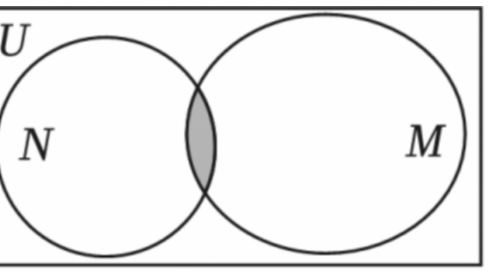
\includegraphics[width=0.30\textwidth]{figures/gao87_q14_venn.png}
\end{center}

\keepwithprev
A. $3$ 个\qquad B. $2$ 个\qquad C. $1$ 个\qquad D. 无穷多个

\ifanswer
\solbegin
\step{阴影部分所示的集合为 $M\cap N$，}
\step{$M=\{x\mid-1\leqslant x\leqslant3\}$，在此范围内的奇数有 $1$ 和 $3$，}
\step{所以集合 $M\cap N=\{1,3\}$ 共有 $2$ 个元素，故选 $B$.}
\solend
\fi

\item 已知实数 $a,b,c$ 满足 $a>b$，则下列不等式成立的是\mbox{（\quad）}

\keepwithprev
A. $-\dfrac1a<\dfrac1b$\qquad B. $a^2>b^2$\qquad C. $a\lvert c\rvert>b\lvert c\rvert$\qquad D. $\dfrac a{c^2+1}>\dfrac b{c^2+1}$

\ifanswer
\solbegin
\step{若 $a=1,b=-1$，则 $-1=-\dfrac1a=\dfrac1b=1$，$a^2=b^2=1$，则 AB 错误；}
\step{若 $a>b,c=0$，则 $a\lvert c\rvert=b\lvert c\rvert=0$，则 C 错误；}
\step{因为 $c^2+1\geqslant1$，所以 $0<\dfrac1{c^2+1}\leqslant1$，又 $a>b$，所以 $\dfrac a{c^2+1}>\dfrac b{c^2+1}$，}
\step{则 D 正确.}
\step{故选 $D$.}
\solend
\fi

\item 设集合 $P_1=\{x\mid x^2+ax+1>0\}$，$P_2=\{x\mid x^2+ax+2>0\}$，$Q_1=\{x\mid x^2+x+b>0\}$，
$Q_2=\{x\mid x^2+2x+b>0\}$，其中 $a$、$b\in\R$，下列说法中正确的是\mbox{（\quad）}

\keepwithprev
A. 对任意 $a$，$P_1$ 是 $P_2$ 的子集，对任意 $b$，$Q_1$ 不是 $Q_2$ 的子集

B. 对任意 $a$，$P_1$ 是 $P_2$ 的子集，存在 $b$，使得 $Q_1$ 是 $Q_2$ 的子集

C. 存在 $a$，使得 $P_1$ 不是 $P_2$ 的子集，对任意 $b$，$Q_1$ 不是 $Q_2$ 的子集

D. 存在 $a$，使得 $P_1$ 不是 $P_2$ 的子集，存在 $b$，使得 $Q_1$ 是 $Q_2$ 的子集

\ifanswer
\solbegin
\step{对于集合 $P_1=\{x\mid x^2+ax+1>0\}$，$P_2=\{x\mid x^2+ax+2>0\}$，}
\step{得当 $m\in P_1$ 时，即 $m^2+am+1>0$，得 $m^2+am+2>0$，}
\step{即有 $m\in P_2$，得对任意 $a$，$P_1$ 是 $P_2$ 的子集，}
\step{对于集合 $Q_1=\{x\mid x^2+x+b>0\}$，$Q_2=\{x\mid x^2+2x+b>0\}$，}
\step{当 $b=6$ 时，$Q_1=\{x\mid x^2+x+6>0\}=\R$，$Q_2=\{x\mid x^2+2x+6>0\}=\R$，}
\step{得 $Q_1$ 是 $Q_2$ 的子集，}
\step{当 $b=1$ 时，$Q_1=\{x\mid x^2+x+1>0\}=\R$，}
\step{$Q_2=\{x\mid x^2+2x+1>0\}=\{x\mid x\neq-1\}$，得 $Q_1$ 不是 $Q_2$ 的子集，}
\step{所以存在 $b$，使得 $Q_1$ 是 $Q_2$ 的子集，故选 $B$.}
\solend
\fi

\end{enumerate}

\bigsec{三、解答题}

\begin{enumerate}
\setcounter{enumi}{16}

\item 设 $m$ 为实数，求关于 $x$ 与 $y$ 的二元一次方程组 $\begin{cases}y=x+m\\ mx-y=4\end{cases}$ 的解集.

\ansspace*[8]

\ifanswer
\solbegin
\step{消去 $y$ 得 $(m-1)x=m+4$，}
\step{当 $m-1=0$，即 $m=1$ 时，$0=5$ 不成立，则 $x$ 无解，原方程组的解集为 $\varnothing$；}
\step{当 $m-1\neq0$，即 $m\neq1$ 时，则 $x=\dfrac{m+4}{m-1}$，$y=\dfrac{m+4}{m-1}+m=\dfrac{m^2+4}{m-1}$，}
\step{原方程组的解集为 $\left\{\left(\dfrac{m+4}{m-1},\dfrac{m^2+4}{m-1}\right)\right\}$.}
\step{综上所述，当 $m=1$ 时，方程组的解集为 $\varnothing$；}
\step{当 $m\neq1$ 时，方程组的解集为 $\left\{\left(\dfrac{m+4}{m-1},\dfrac{m^2+4}{m-1}\right)\right\}$.}
\solend
\fi

\item 设 $x<y<0$，试比较 $(x^2+y^2)(x-y)$ 与 $(x^2-y^2)(x+y)$ 的大小.

\ansspace*[9]

\ifanswer
\solbegin
\step{$(x^2+y^2)(x-y)-(x^2-y^2)(x+y)=(x-y)[x^2+y^2-(x+y)^2]=-2xy(x-y)$，}
\step{因为 $x<y<0$，所以 $xy>0$，$x-y<0$，所以 $-2xy(x-y)>0$，}
\step{即 $(x^2+y^2)(x-y)>(x^2-y^2)(x+y)$.}
\solend
\fi

\item 已知全集 $U=\R$，集合 $A=\left\{x\left|\dfrac{2+x}{3-x}>0\right.\right\}$，集合 $B=\{x\mid\lvert x-2\rvert>3\}$.

（1）求 $A\cup B$、$\overline A\cap B$.

（2）若集合 $C=\{x\mid x\leqslant a\}$，且 $A\cap C=A$，求实数 $a$ 的范围.

\ansspace*[10]

\ifanswer
\solbegin
\stepm{（1）}{由 $\lvert x-2\rvert>3$ 得 $x-2>3$ 或 $x-2<-3$，即 $x<-1$ 或 $x>5$，}
\step{所以 $B=(-\infty,-1)\cup(5,+\infty)$，}
\step{$A=\left\{x\left|\dfrac{2+x}{3-x}>0\right.\right\}=\{x\mid(2+x)(3-x)>0\}=(-2,3)$，}
\step{所以 $A\cup b=(-\infty,3)\cup(5m+\infty)$，}
\step{$\overline A=(-\infty,-2]\cup[3,+\infty)$，$\overline A\cap B=(-\infty,-2]\cup(5,+\infty)$.}
\stepm{（2）}{因为 $A\cap C=A$，所以 $A\subseteq C$，}
\step{因为 $A=(-2,3)$，所以实数 $a$ 的取值范围为 $\{a\mid a\geqslant3\}$.}
\solend
\fi

\item 已知函数 $f(x)=ax^2+4x+b\,(a<0,a,b\in\R)$，设关于 $x$ 的方程 $f(x)=0$ 的两实根为 $x_1$、
$x_2$，方程 $f(x)=x$ 的两实根为 $\alpha,\beta$.

（1）不等式 $f(x)<0$ 的解集是 $(-\infty,-3)\cup(5,+\infty)$，求不等式 $bx^2-ax-4<0$ 的解集；

（2）若 $a,b$ 均为负整数，且 $\lvert\alpha-\beta\rvert=1$，求 $f(x)$ 的解析式.

\ansspace*[12]

\ifanswer
\solbegin
\stepm{（1）}{$ax^2+4x+b<0$ 的解集为 $(-\infty,-3)\cup(5,+\infty)$，}
\step{所以 $-3,5$ 是方程 $ax^2+4x+b=0$ 的两根，所以 $\begin{cases}-3+5=-\dfrac4a\\ -3\times5=\dfrac ba\end{cases}\Rightarrow\begin{cases}a=-2\\ b=30\end{cases}$，}
\step{所以 $bx^2-ax-4<0$ 为 $30x^2+2x-4<0\Rightarrow15x^2+x-2<0$，}
\step{所以 $(3x-1)(5x+2)<0\Rightarrow-\dfrac25<x<\dfrac13$，}
\step{所以所求不等式的解集为 $\left\{x\left|-\dfrac25<x<\dfrac13\right.\right\}$.}
\stepm{（2）}{由题意得 $f(x)=ax^2+4x+b\,(a<0,a,b\in\R)$ 有两个不等实根为 $\alpha$、$\beta$，}
\step{所以 $\Delta=9-4ab>0$，$\alpha+\beta=-\dfrac3a$，$\alpha\beta=\dfrac ba$.}
\step{由 $\lvert\alpha-\beta\rvert=1$ 得 $(\alpha-\beta)^2=1$，即 $(\alpha+\beta)^2-4\alpha\beta=\dfrac9{a^2}-\dfrac{4b}a=1$，}
\step{所以 $9-4ab=a^2$，即 $a^2+4ab=9\,(a<0,a,b\in\R)$.}
\step{因为 $a,b$ 均为负整数，}
\step{所以 $\begin{cases}a=-1\\ a+4b=-9\end{cases}$ 或 $\begin{cases}a=-9\\ a+4b=-1\end{cases}$ 或 $\begin{cases}a=-3\\ a+4b=-3\end{cases}$，}
\step{显然后两种情况不合题意，应舍去，从而有 $\begin{cases}a=-1\\ a+4b=-9\end{cases}$，解得 $a=-1$，$b=-2$.}
\step{故所求函数解析式为 $f(x)=-x^2+4x-2$.}
\solend
\fi

\item 已知集合 $A=\{x\mid x=m^2+n^2,m\in\Z,n\in\Z\}$.

（1）判断 $2,5,25$ 是否属于集合 $A$；

（2）若正整数 $y$ 能表示为某个整数的平方，$z\in A$，证明：$yz\in A$；

（3）若集合 $B=\{x\mid x=4k+3,k\in\Z\}$，证明：$A\cap B=\varnothing$.

\ansspace*[14]

\ifanswer
\solbegin
\stepm{（1）}{由 $2=1^2+1^2$，$5=1^2+2^2$，$25=3^2+4^2$ 得 $2,5,25$ 属于集合 $A$；}
\stepm{（2）}{设 $y=a^2\,(a\in\Z)$，由 $z\in A$，设 $z=b^2+c^2\,(b\in\Z,c\in\Z)$，}
\step{则 $yz=a^2(b^2+c^2)=(ab)^2+(ac)^2$，}
\step{因为 $a\in\Z$，$b\in\Z$，$c\in\Z$，所以 $ab\in\Z$，$ac\in\Z$，所以 $yz\in A$；}
\stepm{（3）}{①当 $m$、$n$ 都为偶数时，设 $m=2k_1\,(k_1\in\Z)$，$n=2k_2\,(k_2\in\Z)$，}
\step{则 $x=m^2+n^2=4k_1^2+4k_2^2=4(k_1^2+k_2^2)$，此时 $x$ 为 $4$ 的倍数，}
\step{因为偶数 $\notin B$，所以 $A\cap B=\varnothing$；}
\step{②当 $m$、$n$ 都为奇数时，设 $m=2k_1+1\,(k_1\in\Z)$，$n=2k_2+1\,(k_2\in\Z)$，}
\step{则 $x=m^2+n^2=(2k_1+1)^2+(2k_2+1)^2=4(k_1^2+k_2^2+k_1+k_2)+2$，}
\step{此时 $x$ 为 $2$ 的倍数，因为偶数 $\notin B$，所以 $A\cap B=\varnothing$；}
\step{③当 $m$、$n$ 一奇一偶时，设 $m=2k_1+1\,(k_1\in\Z)$，$n=2k_2\,(k_2\in\Z)$，}
\step{则 $x=m^2+n^2=(2k_1+1)^2+(2k_2)^2=4(k_1^2+k_2^2+k_1)+1$，}
\step{此时 $x$ 被 $4$ 除余 $1$，而 $B$ 中元素被 $4$ 除余 $3$，此时 $A\cap B=\varnothing$.}
\step{综上，$A\cap B=\varnothing$.}
\solend
\fi

\end{enumerate}

\end{document}
"
%
% 原始材料：微信公众号“魔都数学加油站”文章，连载“27学年高一87”；
% 原文标题“27学年高一87——2026-2027年上海市五十四中学高一上10月月考”；
% 原文链接：https://mp.weixin.qq.com/s/pqPpSGQt0AhydcpaB8uEkQ。
% 页面标注发布时间 2026-10-27 17:43（上海）。
% 正文为 7 张 PNG 页（`原图/高一87_五十四中学_10月月考/01..07.png`），
% 尺寸混排（第 1、2 页为 4762×6735，第 3—7 页为 2560×3620），均按页序读取。
%
% 篇幅与题号：原卷自第 3 题起编号（第 1、2 题不在原文内）。填空题 3—12（10 题）、
% 选择题 13—16（4 题）、解答题 17—21（5 题），共 19 题。
%
% 讲评版：第 3、5、6 题只印【答案】（“$x\leqslant1$ 且 $y\leqslant1$”“$\{(2,6),(6,2)\}$”
% “$(-1,3]$”），本稿只给 \ans{}；其余 16 题印【解析】，其中选择题答案在解析末句
% “故选 A／B／D／B”。第 14 题题干带一幅韦恩图（裁自第 3 页原图、去粉色水印后转灰度），
% 三版都出。
%
% 副标题：原卷未印副标题。本稿按内容标作“集合与常用逻辑用语、不等式”。
%
% 原卷笔误/存疑（均照录未改，正文对应处另有 % 注）：
%   ① 第 19 题 (1) 解析作“所以 $A\cup b=(-\infty,3)\cup(5m+\infty)$”，两处均系排印错：
%      按上下文应为“$A\cup B=(-\infty,3)\cup(5,+\infty)$”（同页下一行 $\overline A\cap B$
%      的端点 $5$、$+\infty$ 也印证这一点）。原卷印作 $b$ 与 $5m+\infty$，照录未改。
%
% 与原卷的排版差异：
%   ① 原卷每题下直接印【答案】/【解析】，本稿按全稿惯例将答案与解析置于答案版；
%   ② 原卷未印副标题，本稿补出；填空横线统一排 \blankline[4.4em]；
%   ③ 原卷数集记号排斜体 $R$、$Z$、$N$，本稿按全稿惯例改用 $\R$、$\Z$、$\N$；
%   ④ 第 17—21 题的子问用行内“（1）（2）（3）”段，解析中的子问标号用 \stepm；
%   ⑤ 解答题按惯例加 \ansspace；选择题括号排 \mbox{（\quad）}。
%
% 行数核对：逐题数 \step/\stepm 条数，合计 86 条（Q4：1；Q7：4；Q8：2；Q9：2；Q10：3；
% Q11：9；Q12：3；Q13：2；Q14：3；Q15：5；Q16：9；Q17：6；Q18：3；Q19：7；Q20：13；
% Q21：14）；第 3、5、6 题只印【答案】，提 \ans{}，不计入 \step 账。原卷解析的换行
% 按语意合并，未逐行强拆。
%
\documentclass[a4paper,11pt]{article}
\usepackage{common}

\begin{document}

\examtitlest[7]{2026--2027 年五十四中学高一上 10 月月考}{集合与常用逻辑用语、不等式}

\bigsec{一、填空题}

\begin{enumerate}
\setcounter{enumi}{2}

\item “$x>1$ 或 $y>1$”的否定形式为\blankline[4.4em].

\ifanswer
\ans{$x\leqslant1$ 且 $y\leqslant1$}
\fi

\item 已知 $1<a<2$，$-3<b<3$，则 $a+b$ 的取值范围是\blankline[4.4em].

\ifanswer
\solbegin
\step{由不等式的可加性得 $-2<a+b<5$，故 $a+b$ 的取值范围是 $(-2,5)$.}
\solend
\fi

\item 方程组 $\begin{cases}x+y=8\\ xy=12\end{cases}$ 的解集为\blankline[4.4em].

\ifanswer
\ans{$\{(2,6),(6,2)\}$}
\fi

\item 不等式 $\dfrac{x-3}{x+1}\leqslant0$ 解集为\blankline[4.4em].

\ifanswer
\ans{$(-1,3]$}
\fi

\item 已知集合 $A=\{x\mid y=\sqrt{x+1}\}$，$B=\{y\mid y=x^2+5\}$，则 $A\cup B=\blankline[4.4em]$.

\ifanswer
\solbegin
\step{对于函数 $y=\sqrt{x+1}$，则 $x+1\geqslant0$，解得 $x\geqslant-1$，}
\step{所以 $A=\{x\mid y=\sqrt{x+1}\}=\{x\mid x\geqslant-1\}$，}
\step{因为 $x^2\geqslant0$，所以 $y=x^2+5\geqslant5$，所以 $B=\{y\mid y=x^2+5\}=\{y\mid y\geqslant5\}$，}
\step{所以 $A\cup B=\{x\mid x\geqslant-1\}$.}
\solend
\fi

\item 已知关于 $x$ 的不等式 $\lvert x+a\rvert<b$ 的解集为 $\{x\mid2<x<4\}$，则 $a+b$ 的值是\blankline[4.4em].

\ifanswer
\solbegin
\step{由 $\lvert x+a\rvert<b$，得 $-b-a<x<b-a$，则 $\begin{cases}-b-a=2\\ b-a=4\end{cases}$，解得 $a=-3$，$b=1$，}
\step{所以 $a+b=-2$.}
\solend
\fi

\item 已知一元二次方程 $x^2-2mx+m-1=0$ 的两实根为 $x_1,x_2$，且 $x_1^2+x_2^2=4$，则实数 $m$ 的值
是\blankline[4.4em].

\ifanswer
\solbegin
\step{由题意得 $x_1+x_2=2m$，$x_1x_2=m-1$，}
\step{所以 $x_1^2+x_2^2=(x_1+x_2)^2-2x_1x_2=4m^2-2m+2=4$，解得 $m=1$ 或 $m=-\dfrac12$.}
\solend
\fi

\item 已知集合 $A=\{x\mid x^2-x-6=0\}$，$B=\{y\mid ay-1=0\}$，若 $A\cap B=B$，则实数
$a=\blankline[4.4em]$.

\ifanswer
\solbegin
\step{$A=\{-2,3\}$，由 $A\cap B=B$，得 $B\subseteq A$，而 $B=\{y\mid ay-1=0\}$，}
\step{则当 $B=\varnothing$ 时，$a=0$；当 $B=\{-2\}$ 时，$-2a-1=0$，解得 $a=-\dfrac12$；}
\step{当 $B=\{3\}$ 时，$3a-1=0$，解得 $a=\dfrac13$，所以实数 $a$ 的值为 $-\dfrac12$ 或 $0$ 或 $\dfrac13$.}
\solend
\fi

\item 已知集合 $A=\{x\mid(m-1)x^2+(m-1)x+2\leqslant0,x\in\R\}$，$B=\left\{x\left|\dfrac{2x-1}{x^2+x+1}>1,x\in\R\right.\right\}$，
且 $A\cap B=A$，则实数 $m$ 的取值范围是\blankline[4.4em].

\ifanswer
\solbegin
\step{因为 $\dfrac{2x-1}{x^2+x+1}>1$，所以 $x^2-x+2<0$，显然不等式无解，}
\step{所以 $B=\left\{x\left|\dfrac{2x-1}{x^2+x+1}>1,x\in\R\right.\right\}=\varnothing$，而 $A\cap B=A$，则 $A=\varnothing$，}
\step{①当 $m=1$ 时，$2\leqslant0$ 不成立，此时 $A=\varnothing$，}
\step{②当 $m<1$ 时，$m-1<0$，函数 $y=(m-1)x^2+(m-1)x+2$，开口向下，}
\step{不等式 $(m-1)x^2+(m-1)x+2\leqslant0$ 有解，$A\neq\varnothing$，}
\step{③当 $m>1$ 时，函数 $y=(m-1)x^2+(m-1)x+2$，开口向上，}
\step{若不等式 $(m-1)x^2+(m-1)x+2\leqslant0$ 无解，}
\step{只需 $\Delta=(m-1)^2-8(m-1)<0$，解得 $1<m<9$，}
\step{综上，$m$ 的取值范围是 $[1,9]$.}
\solend
\fi

\item 设 $A$ 是整数集的一个非空子集，对于 $k\in A$，如果 $k-1\notin A$ 且 $k+1\notin A$，那么 $k$ 是 $A$
的一个“孤立元”. 给定 $S=\{1,2,3,4,5,6,7,8\}$，由 $S$ 的 $3$ 个元素构成的所有集合中，不含
“孤立元”的集合共有\blankline[3.6em]个.

\ifanswer
\solbegin
\step{由题意得，“孤立元”即为在集合中无与之相邻的元素，}
\step{满足条件的集合有 $\{1,2,3\},\{2,3,4\},\{3,4,5\},\{4,5,6\},\{5,6,7\},\{6,7,8\}$，}
\step{共 $6$ 个集合.}
\solend
\fi

\end{enumerate}

\bigsec{二、选择题}

\begin{enumerate}
\setcounter{enumi}{12}

\item “$m=2$”是“$m^2=4$”的\mbox{（\quad）}条件.

\keepwithprev
A. 充分非必要条件\qquad B. 必要非充分条件

C. 充要条件\qquad D. 既非充分又非必要条件

\ifanswer
\solbegin
\step{由 $m^2=4$，解得 $m=\pm2$，故“$m=2$”是“$m^2=4$”的充分不必要条件，}
\step{故选 $A$.}
\solend
\fi

\item 已知全集 $U=\R$，集合 $M=\{x\mid\lvert x-1\rvert\leqslant2\}$ 和 $N=\{x\mid x=2k-1,k\in\Z\}$ 的关系
的韦恩（$Venn$）图如图所示，则阴影部分所示的集合的元素共有\mbox{（\quad）}

\begin{center}
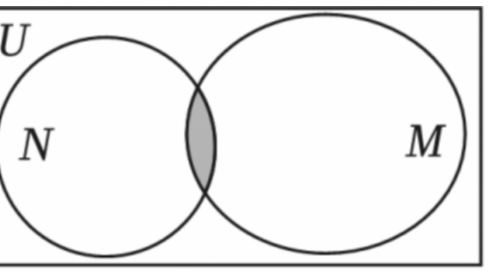
\includegraphics[width=0.30\textwidth]{figures/gao87_q14_venn.png}
\end{center}

\keepwithprev
A. $3$ 个\qquad B. $2$ 个\qquad C. $1$ 个\qquad D. 无穷多个

\ifanswer
\solbegin
\step{阴影部分所示的集合为 $M\cap N$，}
\step{$M=\{x\mid-1\leqslant x\leqslant3\}$，在此范围内的奇数有 $1$ 和 $3$，}
\step{所以集合 $M\cap N=\{1,3\}$ 共有 $2$ 个元素，故选 $B$.}
\solend
\fi

\item 已知实数 $a,b,c$ 满足 $a>b$，则下列不等式成立的是\mbox{（\quad）}

\keepwithprev
A. $-\dfrac1a<\dfrac1b$\qquad B. $a^2>b^2$\qquad C. $a\lvert c\rvert>b\lvert c\rvert$\qquad D. $\dfrac a{c^2+1}>\dfrac b{c^2+1}$

\ifanswer
\solbegin
\step{若 $a=1,b=-1$，则 $-1=-\dfrac1a=\dfrac1b=1$，$a^2=b^2=1$，则 AB 错误；}
\step{若 $a>b,c=0$，则 $a\lvert c\rvert=b\lvert c\rvert=0$，则 C 错误；}
\step{因为 $c^2+1\geqslant1$，所以 $0<\dfrac1{c^2+1}\leqslant1$，又 $a>b$，所以 $\dfrac a{c^2+1}>\dfrac b{c^2+1}$，}
\step{则 D 正确.}
\step{故选 $D$.}
\solend
\fi

\item 设集合 $P_1=\{x\mid x^2+ax+1>0\}$，$P_2=\{x\mid x^2+ax+2>0\}$，$Q_1=\{x\mid x^2+x+b>0\}$，
$Q_2=\{x\mid x^2+2x+b>0\}$，其中 $a$、$b\in\R$，下列说法中正确的是\mbox{（\quad）}

\keepwithprev
A. 对任意 $a$，$P_1$ 是 $P_2$ 的子集，对任意 $b$，$Q_1$ 不是 $Q_2$ 的子集

B. 对任意 $a$，$P_1$ 是 $P_2$ 的子集，存在 $b$，使得 $Q_1$ 是 $Q_2$ 的子集

C. 存在 $a$，使得 $P_1$ 不是 $P_2$ 的子集，对任意 $b$，$Q_1$ 不是 $Q_2$ 的子集

D. 存在 $a$，使得 $P_1$ 不是 $P_2$ 的子集，存在 $b$，使得 $Q_1$ 是 $Q_2$ 的子集

\ifanswer
\solbegin
\step{对于集合 $P_1=\{x\mid x^2+ax+1>0\}$，$P_2=\{x\mid x^2+ax+2>0\}$，}
\step{得当 $m\in P_1$ 时，即 $m^2+am+1>0$，得 $m^2+am+2>0$，}
\step{即有 $m\in P_2$，得对任意 $a$，$P_1$ 是 $P_2$ 的子集，}
\step{对于集合 $Q_1=\{x\mid x^2+x+b>0\}$，$Q_2=\{x\mid x^2+2x+b>0\}$，}
\step{当 $b=6$ 时，$Q_1=\{x\mid x^2+x+6>0\}=\R$，$Q_2=\{x\mid x^2+2x+6>0\}=\R$，}
\step{得 $Q_1$ 是 $Q_2$ 的子集，}
\step{当 $b=1$ 时，$Q_1=\{x\mid x^2+x+1>0\}=\R$，}
\step{$Q_2=\{x\mid x^2+2x+1>0\}=\{x\mid x\neq-1\}$，得 $Q_1$ 不是 $Q_2$ 的子集，}
\step{所以存在 $b$，使得 $Q_1$ 是 $Q_2$ 的子集，故选 $B$.}
\solend
\fi

\end{enumerate}

\bigsec{三、解答题}

\begin{enumerate}
\setcounter{enumi}{16}

\item 设 $m$ 为实数，求关于 $x$ 与 $y$ 的二元一次方程组 $\begin{cases}y=x+m\\ mx-y=4\end{cases}$ 的解集.

\ansspace*[8]

\ifanswer
\solbegin
\step{消去 $y$ 得 $(m-1)x=m+4$，}
\step{当 $m-1=0$，即 $m=1$ 时，$0=5$ 不成立，则 $x$ 无解，原方程组的解集为 $\varnothing$；}
\step{当 $m-1\neq0$，即 $m\neq1$ 时，则 $x=\dfrac{m+4}{m-1}$，$y=\dfrac{m+4}{m-1}+m=\dfrac{m^2+4}{m-1}$，}
\step{原方程组的解集为 $\left\{\left(\dfrac{m+4}{m-1},\dfrac{m^2+4}{m-1}\right)\right\}$.}
\step{综上所述，当 $m=1$ 时，方程组的解集为 $\varnothing$；}
\step{当 $m\neq1$ 时，方程组的解集为 $\left\{\left(\dfrac{m+4}{m-1},\dfrac{m^2+4}{m-1}\right)\right\}$.}
\solend
\fi

\item 设 $x<y<0$，试比较 $(x^2+y^2)(x-y)$ 与 $(x^2-y^2)(x+y)$ 的大小.

\ansspace*[9]

\ifanswer
\solbegin
\step{$(x^2+y^2)(x-y)-(x^2-y^2)(x+y)=(x-y)[x^2+y^2-(x+y)^2]=-2xy(x-y)$，}
\step{因为 $x<y<0$，所以 $xy>0$，$x-y<0$，所以 $-2xy(x-y)>0$，}
\step{即 $(x^2+y^2)(x-y)>(x^2-y^2)(x+y)$.}
\solend
\fi

\item 已知全集 $U=\R$，集合 $A=\left\{x\left|\dfrac{2+x}{3-x}>0\right.\right\}$，集合 $B=\{x\mid\lvert x-2\rvert>3\}$.

（1）求 $A\cup B$、$\overline A\cap B$.

（2）若集合 $C=\{x\mid x\leqslant a\}$，且 $A\cap C=A$，求实数 $a$ 的范围.

\ansspace*[10]

\ifanswer
\solbegin
\stepm{（1）}{由 $\lvert x-2\rvert>3$ 得 $x-2>3$ 或 $x-2<-3$，即 $x<-1$ 或 $x>5$，}
\step{所以 $B=(-\infty,-1)\cup(5,+\infty)$，}
\step{$A=\left\{x\left|\dfrac{2+x}{3-x}>0\right.\right\}=\{x\mid(2+x)(3-x)>0\}=(-2,3)$，}
\step{所以 $A\cup b=(-\infty,3)\cup(5m+\infty)$，}
\step{$\overline A=(-\infty,-2]\cup[3,+\infty)$，$\overline A\cap B=(-\infty,-2]\cup(5,+\infty)$.}
\stepm{（2）}{因为 $A\cap C=A$，所以 $A\subseteq C$，}
\step{因为 $A=(-2,3)$，所以实数 $a$ 的取值范围为 $\{a\mid a\geqslant3\}$.}
\solend
\fi

\item 已知函数 $f(x)=ax^2+4x+b\,(a<0,a,b\in\R)$，设关于 $x$ 的方程 $f(x)=0$ 的两实根为 $x_1$、
$x_2$，方程 $f(x)=x$ 的两实根为 $\alpha,\beta$.

（1）不等式 $f(x)<0$ 的解集是 $(-\infty,-3)\cup(5,+\infty)$，求不等式 $bx^2-ax-4<0$ 的解集；

（2）若 $a,b$ 均为负整数，且 $\lvert\alpha-\beta\rvert=1$，求 $f(x)$ 的解析式.

\ansspace*[12]

\ifanswer
\solbegin
\stepm{（1）}{$ax^2+4x+b<0$ 的解集为 $(-\infty,-3)\cup(5,+\infty)$，}
\step{所以 $-3,5$ 是方程 $ax^2+4x+b=0$ 的两根，所以 $\begin{cases}-3+5=-\dfrac4a\\ -3\times5=\dfrac ba\end{cases}\Rightarrow\begin{cases}a=-2\\ b=30\end{cases}$，}
\step{所以 $bx^2-ax-4<0$ 为 $30x^2+2x-4<0\Rightarrow15x^2+x-2<0$，}
\step{所以 $(3x-1)(5x+2)<0\Rightarrow-\dfrac25<x<\dfrac13$，}
\step{所以所求不等式的解集为 $\left\{x\left|-\dfrac25<x<\dfrac13\right.\right\}$.}
\stepm{（2）}{由题意得 $f(x)=ax^2+4x+b\,(a<0,a,b\in\R)$ 有两个不等实根为 $\alpha$、$\beta$，}
\step{所以 $\Delta=9-4ab>0$，$\alpha+\beta=-\dfrac3a$，$\alpha\beta=\dfrac ba$.}
\step{由 $\lvert\alpha-\beta\rvert=1$ 得 $(\alpha-\beta)^2=1$，即 $(\alpha+\beta)^2-4\alpha\beta=\dfrac9{a^2}-\dfrac{4b}a=1$，}
\step{所以 $9-4ab=a^2$，即 $a^2+4ab=9\,(a<0,a,b\in\R)$.}
\step{因为 $a,b$ 均为负整数，}
\step{所以 $\begin{cases}a=-1\\ a+4b=-9\end{cases}$ 或 $\begin{cases}a=-9\\ a+4b=-1\end{cases}$ 或 $\begin{cases}a=-3\\ a+4b=-3\end{cases}$，}
\step{显然后两种情况不合题意，应舍去，从而有 $\begin{cases}a=-1\\ a+4b=-9\end{cases}$，解得 $a=-1$，$b=-2$.}
\step{故所求函数解析式为 $f(x)=-x^2+4x-2$.}
\solend
\fi

\item 已知集合 $A=\{x\mid x=m^2+n^2,m\in\Z,n\in\Z\}$.

（1）判断 $2,5,25$ 是否属于集合 $A$；

（2）若正整数 $y$ 能表示为某个整数的平方，$z\in A$，证明：$yz\in A$；

（3）若集合 $B=\{x\mid x=4k+3,k\in\Z\}$，证明：$A\cap B=\varnothing$.

\ansspace*[14]

\ifanswer
\solbegin
\stepm{（1）}{由 $2=1^2+1^2$，$5=1^2+2^2$，$25=3^2+4^2$ 得 $2,5,25$ 属于集合 $A$；}
\stepm{（2）}{设 $y=a^2\,(a\in\Z)$，由 $z\in A$，设 $z=b^2+c^2\,(b\in\Z,c\in\Z)$，}
\step{则 $yz=a^2(b^2+c^2)=(ab)^2+(ac)^2$，}
\step{因为 $a\in\Z$，$b\in\Z$，$c\in\Z$，所以 $ab\in\Z$，$ac\in\Z$，所以 $yz\in A$；}
\stepm{（3）}{①当 $m$、$n$ 都为偶数时，设 $m=2k_1\,(k_1\in\Z)$，$n=2k_2\,(k_2\in\Z)$，}
\step{则 $x=m^2+n^2=4k_1^2+4k_2^2=4(k_1^2+k_2^2)$，此时 $x$ 为 $4$ 的倍数，}
\step{因为偶数 $\notin B$，所以 $A\cap B=\varnothing$；}
\step{②当 $m$、$n$ 都为奇数时，设 $m=2k_1+1\,(k_1\in\Z)$，$n=2k_2+1\,(k_2\in\Z)$，}
\step{则 $x=m^2+n^2=(2k_1+1)^2+(2k_2+1)^2=4(k_1^2+k_2^2+k_1+k_2)+2$，}
\step{此时 $x$ 为 $2$ 的倍数，因为偶数 $\notin B$，所以 $A\cap B=\varnothing$；}
\step{③当 $m$、$n$ 一奇一偶时，设 $m=2k_1+1\,(k_1\in\Z)$，$n=2k_2\,(k_2\in\Z)$，}
\step{则 $x=m^2+n^2=(2k_1+1)^2+(2k_2)^2=4(k_1^2+k_2^2+k_1)+1$，}
\step{此时 $x$ 被 $4$ 除余 $1$，而 $B$ 中元素被 $4$ 除余 $3$，此时 $A\cap B=\varnothing$.}
\step{综上，$A\cap B=\varnothing$.}
\solend
\fi

\end{enumerate}

\end{document}
"
% 紧凑版：xelatex "\def\iscompact{1}% 高一87_五十四中学_10月月考.tex
%   —— 高一上数学“2026-2027 年五十四中学高一上 10 月月考”（讲评版）
% 试卷版：xelatex 高一87_五十四中学_10月月考.tex
% 答案版：xelatex "\def\isanswer{1}% 高一87_五十四中学_10月月考.tex
%   —— 高一上数学“2026-2027 年五十四中学高一上 10 月月考”（讲评版）
% 试卷版：xelatex 高一87_五十四中学_10月月考.tex
% 答案版：xelatex "\def\isanswer{1}\input{高一87_五十四中学_10月月考.tex}"
% 紧凑版：xelatex "\def\iscompact{1}\input{高一87_五十四中学_10月月考.tex}"
%
% 原始材料：微信公众号“魔都数学加油站”文章，连载“27学年高一87”；
% 原文标题“27学年高一87——2026-2027年上海市五十四中学高一上10月月考”；
% 原文链接：https://mp.weixin.qq.com/s/pqPpSGQt0AhydcpaB8uEkQ。
% 页面标注发布时间 2026-10-27 17:43（上海）。
% 正文为 7 张 PNG 页（`原图/高一87_五十四中学_10月月考/01..07.png`），
% 尺寸混排（第 1、2 页为 4762×6735，第 3—7 页为 2560×3620），均按页序读取。
%
% 篇幅与题号：原卷自第 3 题起编号（第 1、2 题不在原文内）。填空题 3—12（10 题）、
% 选择题 13—16（4 题）、解答题 17—21（5 题），共 19 题。
%
% 讲评版：第 3、5、6 题只印【答案】（“$x\leqslant1$ 且 $y\leqslant1$”“$\{(2,6),(6,2)\}$”
% “$(-1,3]$”），本稿只给 \ans{}；其余 16 题印【解析】，其中选择题答案在解析末句
% “故选 A／B／D／B”。第 14 题题干带一幅韦恩图（裁自第 3 页原图、去粉色水印后转灰度），
% 三版都出。
%
% 副标题：原卷未印副标题。本稿按内容标作“集合与常用逻辑用语、不等式”。
%
% 原卷笔误/存疑（均照录未改，正文对应处另有 % 注）：
%   ① 第 19 题 (1) 解析作“所以 $A\cup b=(-\infty,3)\cup(5m+\infty)$”，两处均系排印错：
%      按上下文应为“$A\cup B=(-\infty,3)\cup(5,+\infty)$”（同页下一行 $\overline A\cap B$
%      的端点 $5$、$+\infty$ 也印证这一点）。原卷印作 $b$ 与 $5m+\infty$，照录未改。
%
% 与原卷的排版差异：
%   ① 原卷每题下直接印【答案】/【解析】，本稿按全稿惯例将答案与解析置于答案版；
%   ② 原卷未印副标题，本稿补出；填空横线统一排 \blankline[4.4em]；
%   ③ 原卷数集记号排斜体 $R$、$Z$、$N$，本稿按全稿惯例改用 $\R$、$\Z$、$\N$；
%   ④ 第 17—21 题的子问用行内“（1）（2）（3）”段，解析中的子问标号用 \stepm；
%   ⑤ 解答题按惯例加 \ansspace；选择题括号排 \mbox{（\quad）}。
%
% 行数核对：逐题数 \step/\stepm 条数，合计 86 条（Q4：1；Q7：4；Q8：2；Q9：2；Q10：3；
% Q11：9；Q12：3；Q13：2；Q14：3；Q15：5；Q16：9；Q17：6；Q18：3；Q19：7；Q20：13；
% Q21：14）；第 3、5、6 题只印【答案】，提 \ans{}，不计入 \step 账。原卷解析的换行
% 按语意合并，未逐行强拆。
%
\documentclass[a4paper,11pt]{article}
\usepackage{common}

\begin{document}

\examtitlest[7]{2026--2027 年五十四中学高一上 10 月月考}{集合与常用逻辑用语、不等式}

\bigsec{一、填空题}

\begin{enumerate}
\setcounter{enumi}{2}

\item “$x>1$ 或 $y>1$”的否定形式为\blankline[4.4em].

\ifanswer
\ans{$x\leqslant1$ 且 $y\leqslant1$}
\fi

\item 已知 $1<a<2$，$-3<b<3$，则 $a+b$ 的取值范围是\blankline[4.4em].

\ifanswer
\solbegin
\step{由不等式的可加性得 $-2<a+b<5$，故 $a+b$ 的取值范围是 $(-2,5)$.}
\solend
\fi

\item 方程组 $\begin{cases}x+y=8\\ xy=12\end{cases}$ 的解集为\blankline[4.4em].

\ifanswer
\ans{$\{(2,6),(6,2)\}$}
\fi

\item 不等式 $\dfrac{x-3}{x+1}\leqslant0$ 解集为\blankline[4.4em].

\ifanswer
\ans{$(-1,3]$}
\fi

\item 已知集合 $A=\{x\mid y=\sqrt{x+1}\}$，$B=\{y\mid y=x^2+5\}$，则 $A\cup B=\blankline[4.4em]$.

\ifanswer
\solbegin
\step{对于函数 $y=\sqrt{x+1}$，则 $x+1\geqslant0$，解得 $x\geqslant-1$，}
\step{所以 $A=\{x\mid y=\sqrt{x+1}\}=\{x\mid x\geqslant-1\}$，}
\step{因为 $x^2\geqslant0$，所以 $y=x^2+5\geqslant5$，所以 $B=\{y\mid y=x^2+5\}=\{y\mid y\geqslant5\}$，}
\step{所以 $A\cup B=\{x\mid x\geqslant-1\}$.}
\solend
\fi

\item 已知关于 $x$ 的不等式 $\lvert x+a\rvert<b$ 的解集为 $\{x\mid2<x<4\}$，则 $a+b$ 的值是\blankline[4.4em].

\ifanswer
\solbegin
\step{由 $\lvert x+a\rvert<b$，得 $-b-a<x<b-a$，则 $\begin{cases}-b-a=2\\ b-a=4\end{cases}$，解得 $a=-3$，$b=1$，}
\step{所以 $a+b=-2$.}
\solend
\fi

\item 已知一元二次方程 $x^2-2mx+m-1=0$ 的两实根为 $x_1,x_2$，且 $x_1^2+x_2^2=4$，则实数 $m$ 的值
是\blankline[4.4em].

\ifanswer
\solbegin
\step{由题意得 $x_1+x_2=2m$，$x_1x_2=m-1$，}
\step{所以 $x_1^2+x_2^2=(x_1+x_2)^2-2x_1x_2=4m^2-2m+2=4$，解得 $m=1$ 或 $m=-\dfrac12$.}
\solend
\fi

\item 已知集合 $A=\{x\mid x^2-x-6=0\}$，$B=\{y\mid ay-1=0\}$，若 $A\cap B=B$，则实数
$a=\blankline[4.4em]$.

\ifanswer
\solbegin
\step{$A=\{-2,3\}$，由 $A\cap B=B$，得 $B\subseteq A$，而 $B=\{y\mid ay-1=0\}$，}
\step{则当 $B=\varnothing$ 时，$a=0$；当 $B=\{-2\}$ 时，$-2a-1=0$，解得 $a=-\dfrac12$；}
\step{当 $B=\{3\}$ 时，$3a-1=0$，解得 $a=\dfrac13$，所以实数 $a$ 的值为 $-\dfrac12$ 或 $0$ 或 $\dfrac13$.}
\solend
\fi

\item 已知集合 $A=\{x\mid(m-1)x^2+(m-1)x+2\leqslant0,x\in\R\}$，$B=\left\{x\left|\dfrac{2x-1}{x^2+x+1}>1,x\in\R\right.\right\}$，
且 $A\cap B=A$，则实数 $m$ 的取值范围是\blankline[4.4em].

\ifanswer
\solbegin
\step{因为 $\dfrac{2x-1}{x^2+x+1}>1$，所以 $x^2-x+2<0$，显然不等式无解，}
\step{所以 $B=\left\{x\left|\dfrac{2x-1}{x^2+x+1}>1,x\in\R\right.\right\}=\varnothing$，而 $A\cap B=A$，则 $A=\varnothing$，}
\step{①当 $m=1$ 时，$2\leqslant0$ 不成立，此时 $A=\varnothing$，}
\step{②当 $m<1$ 时，$m-1<0$，函数 $y=(m-1)x^2+(m-1)x+2$，开口向下，}
\step{不等式 $(m-1)x^2+(m-1)x+2\leqslant0$ 有解，$A\neq\varnothing$，}
\step{③当 $m>1$ 时，函数 $y=(m-1)x^2+(m-1)x+2$，开口向上，}
\step{若不等式 $(m-1)x^2+(m-1)x+2\leqslant0$ 无解，}
\step{只需 $\Delta=(m-1)^2-8(m-1)<0$，解得 $1<m<9$，}
\step{综上，$m$ 的取值范围是 $[1,9]$.}
\solend
\fi

\item 设 $A$ 是整数集的一个非空子集，对于 $k\in A$，如果 $k-1\notin A$ 且 $k+1\notin A$，那么 $k$ 是 $A$
的一个“孤立元”. 给定 $S=\{1,2,3,4,5,6,7,8\}$，由 $S$ 的 $3$ 个元素构成的所有集合中，不含
“孤立元”的集合共有\blankline[3.6em]个.

\ifanswer
\solbegin
\step{由题意得，“孤立元”即为在集合中无与之相邻的元素，}
\step{满足条件的集合有 $\{1,2,3\},\{2,3,4\},\{3,4,5\},\{4,5,6\},\{5,6,7\},\{6,7,8\}$，}
\step{共 $6$ 个集合.}
\solend
\fi

\end{enumerate}

\bigsec{二、选择题}

\begin{enumerate}
\setcounter{enumi}{12}

\item “$m=2$”是“$m^2=4$”的\mbox{（\quad）}条件.

\keepwithprev
A. 充分非必要条件\qquad B. 必要非充分条件

C. 充要条件\qquad D. 既非充分又非必要条件

\ifanswer
\solbegin
\step{由 $m^2=4$，解得 $m=\pm2$，故“$m=2$”是“$m^2=4$”的充分不必要条件，}
\step{故选 $A$.}
\solend
\fi

\item 已知全集 $U=\R$，集合 $M=\{x\mid\lvert x-1\rvert\leqslant2\}$ 和 $N=\{x\mid x=2k-1,k\in\Z\}$ 的关系
的韦恩（$Venn$）图如图所示，则阴影部分所示的集合的元素共有\mbox{（\quad）}

\begin{center}
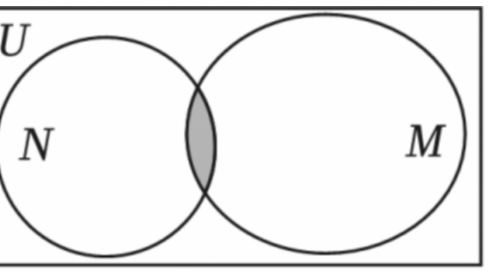
\includegraphics[width=0.30\textwidth]{figures/gao87_q14_venn.png}
\end{center}

\keepwithprev
A. $3$ 个\qquad B. $2$ 个\qquad C. $1$ 个\qquad D. 无穷多个

\ifanswer
\solbegin
\step{阴影部分所示的集合为 $M\cap N$，}
\step{$M=\{x\mid-1\leqslant x\leqslant3\}$，在此范围内的奇数有 $1$ 和 $3$，}
\step{所以集合 $M\cap N=\{1,3\}$ 共有 $2$ 个元素，故选 $B$.}
\solend
\fi

\item 已知实数 $a,b,c$ 满足 $a>b$，则下列不等式成立的是\mbox{（\quad）}

\keepwithprev
A. $-\dfrac1a<\dfrac1b$\qquad B. $a^2>b^2$\qquad C. $a\lvert c\rvert>b\lvert c\rvert$\qquad D. $\dfrac a{c^2+1}>\dfrac b{c^2+1}$

\ifanswer
\solbegin
\step{若 $a=1,b=-1$，则 $-1=-\dfrac1a=\dfrac1b=1$，$a^2=b^2=1$，则 AB 错误；}
\step{若 $a>b,c=0$，则 $a\lvert c\rvert=b\lvert c\rvert=0$，则 C 错误；}
\step{因为 $c^2+1\geqslant1$，所以 $0<\dfrac1{c^2+1}\leqslant1$，又 $a>b$，所以 $\dfrac a{c^2+1}>\dfrac b{c^2+1}$，}
\step{则 D 正确.}
\step{故选 $D$.}
\solend
\fi

\item 设集合 $P_1=\{x\mid x^2+ax+1>0\}$，$P_2=\{x\mid x^2+ax+2>0\}$，$Q_1=\{x\mid x^2+x+b>0\}$，
$Q_2=\{x\mid x^2+2x+b>0\}$，其中 $a$、$b\in\R$，下列说法中正确的是\mbox{（\quad）}

\keepwithprev
A. 对任意 $a$，$P_1$ 是 $P_2$ 的子集，对任意 $b$，$Q_1$ 不是 $Q_2$ 的子集

B. 对任意 $a$，$P_1$ 是 $P_2$ 的子集，存在 $b$，使得 $Q_1$ 是 $Q_2$ 的子集

C. 存在 $a$，使得 $P_1$ 不是 $P_2$ 的子集，对任意 $b$，$Q_1$ 不是 $Q_2$ 的子集

D. 存在 $a$，使得 $P_1$ 不是 $P_2$ 的子集，存在 $b$，使得 $Q_1$ 是 $Q_2$ 的子集

\ifanswer
\solbegin
\step{对于集合 $P_1=\{x\mid x^2+ax+1>0\}$，$P_2=\{x\mid x^2+ax+2>0\}$，}
\step{得当 $m\in P_1$ 时，即 $m^2+am+1>0$，得 $m^2+am+2>0$，}
\step{即有 $m\in P_2$，得对任意 $a$，$P_1$ 是 $P_2$ 的子集，}
\step{对于集合 $Q_1=\{x\mid x^2+x+b>0\}$，$Q_2=\{x\mid x^2+2x+b>0\}$，}
\step{当 $b=6$ 时，$Q_1=\{x\mid x^2+x+6>0\}=\R$，$Q_2=\{x\mid x^2+2x+6>0\}=\R$，}
\step{得 $Q_1$ 是 $Q_2$ 的子集，}
\step{当 $b=1$ 时，$Q_1=\{x\mid x^2+x+1>0\}=\R$，}
\step{$Q_2=\{x\mid x^2+2x+1>0\}=\{x\mid x\neq-1\}$，得 $Q_1$ 不是 $Q_2$ 的子集，}
\step{所以存在 $b$，使得 $Q_1$ 是 $Q_2$ 的子集，故选 $B$.}
\solend
\fi

\end{enumerate}

\bigsec{三、解答题}

\begin{enumerate}
\setcounter{enumi}{16}

\item 设 $m$ 为实数，求关于 $x$ 与 $y$ 的二元一次方程组 $\begin{cases}y=x+m\\ mx-y=4\end{cases}$ 的解集.

\ansspace*[8]

\ifanswer
\solbegin
\step{消去 $y$ 得 $(m-1)x=m+4$，}
\step{当 $m-1=0$，即 $m=1$ 时，$0=5$ 不成立，则 $x$ 无解，原方程组的解集为 $\varnothing$；}
\step{当 $m-1\neq0$，即 $m\neq1$ 时，则 $x=\dfrac{m+4}{m-1}$，$y=\dfrac{m+4}{m-1}+m=\dfrac{m^2+4}{m-1}$，}
\step{原方程组的解集为 $\left\{\left(\dfrac{m+4}{m-1},\dfrac{m^2+4}{m-1}\right)\right\}$.}
\step{综上所述，当 $m=1$ 时，方程组的解集为 $\varnothing$；}
\step{当 $m\neq1$ 时，方程组的解集为 $\left\{\left(\dfrac{m+4}{m-1},\dfrac{m^2+4}{m-1}\right)\right\}$.}
\solend
\fi

\item 设 $x<y<0$，试比较 $(x^2+y^2)(x-y)$ 与 $(x^2-y^2)(x+y)$ 的大小.

\ansspace*[9]

\ifanswer
\solbegin
\step{$(x^2+y^2)(x-y)-(x^2-y^2)(x+y)=(x-y)[x^2+y^2-(x+y)^2]=-2xy(x-y)$，}
\step{因为 $x<y<0$，所以 $xy>0$，$x-y<0$，所以 $-2xy(x-y)>0$，}
\step{即 $(x^2+y^2)(x-y)>(x^2-y^2)(x+y)$.}
\solend
\fi

\item 已知全集 $U=\R$，集合 $A=\left\{x\left|\dfrac{2+x}{3-x}>0\right.\right\}$，集合 $B=\{x\mid\lvert x-2\rvert>3\}$.

（1）求 $A\cup B$、$\overline A\cap B$.

（2）若集合 $C=\{x\mid x\leqslant a\}$，且 $A\cap C=A$，求实数 $a$ 的范围.

\ansspace*[10]

\ifanswer
\solbegin
\stepm{（1）}{由 $\lvert x-2\rvert>3$ 得 $x-2>3$ 或 $x-2<-3$，即 $x<-1$ 或 $x>5$，}
\step{所以 $B=(-\infty,-1)\cup(5,+\infty)$，}
\step{$A=\left\{x\left|\dfrac{2+x}{3-x}>0\right.\right\}=\{x\mid(2+x)(3-x)>0\}=(-2,3)$，}
\step{所以 $A\cup b=(-\infty,3)\cup(5m+\infty)$，}
\step{$\overline A=(-\infty,-2]\cup[3,+\infty)$，$\overline A\cap B=(-\infty,-2]\cup(5,+\infty)$.}
\stepm{（2）}{因为 $A\cap C=A$，所以 $A\subseteq C$，}
\step{因为 $A=(-2,3)$，所以实数 $a$ 的取值范围为 $\{a\mid a\geqslant3\}$.}
\solend
\fi

\item 已知函数 $f(x)=ax^2+4x+b\,(a<0,a,b\in\R)$，设关于 $x$ 的方程 $f(x)=0$ 的两实根为 $x_1$、
$x_2$，方程 $f(x)=x$ 的两实根为 $\alpha,\beta$.

（1）不等式 $f(x)<0$ 的解集是 $(-\infty,-3)\cup(5,+\infty)$，求不等式 $bx^2-ax-4<0$ 的解集；

（2）若 $a,b$ 均为负整数，且 $\lvert\alpha-\beta\rvert=1$，求 $f(x)$ 的解析式.

\ansspace*[12]

\ifanswer
\solbegin
\stepm{（1）}{$ax^2+4x+b<0$ 的解集为 $(-\infty,-3)\cup(5,+\infty)$，}
\step{所以 $-3,5$ 是方程 $ax^2+4x+b=0$ 的两根，所以 $\begin{cases}-3+5=-\dfrac4a\\ -3\times5=\dfrac ba\end{cases}\Rightarrow\begin{cases}a=-2\\ b=30\end{cases}$，}
\step{所以 $bx^2-ax-4<0$ 为 $30x^2+2x-4<0\Rightarrow15x^2+x-2<0$，}
\step{所以 $(3x-1)(5x+2)<0\Rightarrow-\dfrac25<x<\dfrac13$，}
\step{所以所求不等式的解集为 $\left\{x\left|-\dfrac25<x<\dfrac13\right.\right\}$.}
\stepm{（2）}{由题意得 $f(x)=ax^2+4x+b\,(a<0,a,b\in\R)$ 有两个不等实根为 $\alpha$、$\beta$，}
\step{所以 $\Delta=9-4ab>0$，$\alpha+\beta=-\dfrac3a$，$\alpha\beta=\dfrac ba$.}
\step{由 $\lvert\alpha-\beta\rvert=1$ 得 $(\alpha-\beta)^2=1$，即 $(\alpha+\beta)^2-4\alpha\beta=\dfrac9{a^2}-\dfrac{4b}a=1$，}
\step{所以 $9-4ab=a^2$，即 $a^2+4ab=9\,(a<0,a,b\in\R)$.}
\step{因为 $a,b$ 均为负整数，}
\step{所以 $\begin{cases}a=-1\\ a+4b=-9\end{cases}$ 或 $\begin{cases}a=-9\\ a+4b=-1\end{cases}$ 或 $\begin{cases}a=-3\\ a+4b=-3\end{cases}$，}
\step{显然后两种情况不合题意，应舍去，从而有 $\begin{cases}a=-1\\ a+4b=-9\end{cases}$，解得 $a=-1$，$b=-2$.}
\step{故所求函数解析式为 $f(x)=-x^2+4x-2$.}
\solend
\fi

\item 已知集合 $A=\{x\mid x=m^2+n^2,m\in\Z,n\in\Z\}$.

（1）判断 $2,5,25$ 是否属于集合 $A$；

（2）若正整数 $y$ 能表示为某个整数的平方，$z\in A$，证明：$yz\in A$；

（3）若集合 $B=\{x\mid x=4k+3,k\in\Z\}$，证明：$A\cap B=\varnothing$.

\ansspace*[14]

\ifanswer
\solbegin
\stepm{（1）}{由 $2=1^2+1^2$，$5=1^2+2^2$，$25=3^2+4^2$ 得 $2,5,25$ 属于集合 $A$；}
\stepm{（2）}{设 $y=a^2\,(a\in\Z)$，由 $z\in A$，设 $z=b^2+c^2\,(b\in\Z,c\in\Z)$，}
\step{则 $yz=a^2(b^2+c^2)=(ab)^2+(ac)^2$，}
\step{因为 $a\in\Z$，$b\in\Z$，$c\in\Z$，所以 $ab\in\Z$，$ac\in\Z$，所以 $yz\in A$；}
\stepm{（3）}{①当 $m$、$n$ 都为偶数时，设 $m=2k_1\,(k_1\in\Z)$，$n=2k_2\,(k_2\in\Z)$，}
\step{则 $x=m^2+n^2=4k_1^2+4k_2^2=4(k_1^2+k_2^2)$，此时 $x$ 为 $4$ 的倍数，}
\step{因为偶数 $\notin B$，所以 $A\cap B=\varnothing$；}
\step{②当 $m$、$n$ 都为奇数时，设 $m=2k_1+1\,(k_1\in\Z)$，$n=2k_2+1\,(k_2\in\Z)$，}
\step{则 $x=m^2+n^2=(2k_1+1)^2+(2k_2+1)^2=4(k_1^2+k_2^2+k_1+k_2)+2$，}
\step{此时 $x$ 为 $2$ 的倍数，因为偶数 $\notin B$，所以 $A\cap B=\varnothing$；}
\step{③当 $m$、$n$ 一奇一偶时，设 $m=2k_1+1\,(k_1\in\Z)$，$n=2k_2\,(k_2\in\Z)$，}
\step{则 $x=m^2+n^2=(2k_1+1)^2+(2k_2)^2=4(k_1^2+k_2^2+k_1)+1$，}
\step{此时 $x$ 被 $4$ 除余 $1$，而 $B$ 中元素被 $4$ 除余 $3$，此时 $A\cap B=\varnothing$.}
\step{综上，$A\cap B=\varnothing$.}
\solend
\fi

\end{enumerate}

\end{document}
"
% 紧凑版：xelatex "\def\iscompact{1}% 高一87_五十四中学_10月月考.tex
%   —— 高一上数学“2026-2027 年五十四中学高一上 10 月月考”（讲评版）
% 试卷版：xelatex 高一87_五十四中学_10月月考.tex
% 答案版：xelatex "\def\isanswer{1}\input{高一87_五十四中学_10月月考.tex}"
% 紧凑版：xelatex "\def\iscompact{1}\input{高一87_五十四中学_10月月考.tex}"
%
% 原始材料：微信公众号“魔都数学加油站”文章，连载“27学年高一87”；
% 原文标题“27学年高一87——2026-2027年上海市五十四中学高一上10月月考”；
% 原文链接：https://mp.weixin.qq.com/s/pqPpSGQt0AhydcpaB8uEkQ。
% 页面标注发布时间 2026-10-27 17:43（上海）。
% 正文为 7 张 PNG 页（`原图/高一87_五十四中学_10月月考/01..07.png`），
% 尺寸混排（第 1、2 页为 4762×6735，第 3—7 页为 2560×3620），均按页序读取。
%
% 篇幅与题号：原卷自第 3 题起编号（第 1、2 题不在原文内）。填空题 3—12（10 题）、
% 选择题 13—16（4 题）、解答题 17—21（5 题），共 19 题。
%
% 讲评版：第 3、5、6 题只印【答案】（“$x\leqslant1$ 且 $y\leqslant1$”“$\{(2,6),(6,2)\}$”
% “$(-1,3]$”），本稿只给 \ans{}；其余 16 题印【解析】，其中选择题答案在解析末句
% “故选 A／B／D／B”。第 14 题题干带一幅韦恩图（裁自第 3 页原图、去粉色水印后转灰度），
% 三版都出。
%
% 副标题：原卷未印副标题。本稿按内容标作“集合与常用逻辑用语、不等式”。
%
% 原卷笔误/存疑（均照录未改，正文对应处另有 % 注）：
%   ① 第 19 题 (1) 解析作“所以 $A\cup b=(-\infty,3)\cup(5m+\infty)$”，两处均系排印错：
%      按上下文应为“$A\cup B=(-\infty,3)\cup(5,+\infty)$”（同页下一行 $\overline A\cap B$
%      的端点 $5$、$+\infty$ 也印证这一点）。原卷印作 $b$ 与 $5m+\infty$，照录未改。
%
% 与原卷的排版差异：
%   ① 原卷每题下直接印【答案】/【解析】，本稿按全稿惯例将答案与解析置于答案版；
%   ② 原卷未印副标题，本稿补出；填空横线统一排 \blankline[4.4em]；
%   ③ 原卷数集记号排斜体 $R$、$Z$、$N$，本稿按全稿惯例改用 $\R$、$\Z$、$\N$；
%   ④ 第 17—21 题的子问用行内“（1）（2）（3）”段，解析中的子问标号用 \stepm；
%   ⑤ 解答题按惯例加 \ansspace；选择题括号排 \mbox{（\quad）}。
%
% 行数核对：逐题数 \step/\stepm 条数，合计 86 条（Q4：1；Q7：4；Q8：2；Q9：2；Q10：3；
% Q11：9；Q12：3；Q13：2；Q14：3；Q15：5；Q16：9；Q17：6；Q18：3；Q19：7；Q20：13；
% Q21：14）；第 3、5、6 题只印【答案】，提 \ans{}，不计入 \step 账。原卷解析的换行
% 按语意合并，未逐行强拆。
%
\documentclass[a4paper,11pt]{article}
\usepackage{common}

\begin{document}

\examtitlest[7]{2026--2027 年五十四中学高一上 10 月月考}{集合与常用逻辑用语、不等式}

\bigsec{一、填空题}

\begin{enumerate}
\setcounter{enumi}{2}

\item “$x>1$ 或 $y>1$”的否定形式为\blankline[4.4em].

\ifanswer
\ans{$x\leqslant1$ 且 $y\leqslant1$}
\fi

\item 已知 $1<a<2$，$-3<b<3$，则 $a+b$ 的取值范围是\blankline[4.4em].

\ifanswer
\solbegin
\step{由不等式的可加性得 $-2<a+b<5$，故 $a+b$ 的取值范围是 $(-2,5)$.}
\solend
\fi

\item 方程组 $\begin{cases}x+y=8\\ xy=12\end{cases}$ 的解集为\blankline[4.4em].

\ifanswer
\ans{$\{(2,6),(6,2)\}$}
\fi

\item 不等式 $\dfrac{x-3}{x+1}\leqslant0$ 解集为\blankline[4.4em].

\ifanswer
\ans{$(-1,3]$}
\fi

\item 已知集合 $A=\{x\mid y=\sqrt{x+1}\}$，$B=\{y\mid y=x^2+5\}$，则 $A\cup B=\blankline[4.4em]$.

\ifanswer
\solbegin
\step{对于函数 $y=\sqrt{x+1}$，则 $x+1\geqslant0$，解得 $x\geqslant-1$，}
\step{所以 $A=\{x\mid y=\sqrt{x+1}\}=\{x\mid x\geqslant-1\}$，}
\step{因为 $x^2\geqslant0$，所以 $y=x^2+5\geqslant5$，所以 $B=\{y\mid y=x^2+5\}=\{y\mid y\geqslant5\}$，}
\step{所以 $A\cup B=\{x\mid x\geqslant-1\}$.}
\solend
\fi

\item 已知关于 $x$ 的不等式 $\lvert x+a\rvert<b$ 的解集为 $\{x\mid2<x<4\}$，则 $a+b$ 的值是\blankline[4.4em].

\ifanswer
\solbegin
\step{由 $\lvert x+a\rvert<b$，得 $-b-a<x<b-a$，则 $\begin{cases}-b-a=2\\ b-a=4\end{cases}$，解得 $a=-3$，$b=1$，}
\step{所以 $a+b=-2$.}
\solend
\fi

\item 已知一元二次方程 $x^2-2mx+m-1=0$ 的两实根为 $x_1,x_2$，且 $x_1^2+x_2^2=4$，则实数 $m$ 的值
是\blankline[4.4em].

\ifanswer
\solbegin
\step{由题意得 $x_1+x_2=2m$，$x_1x_2=m-1$，}
\step{所以 $x_1^2+x_2^2=(x_1+x_2)^2-2x_1x_2=4m^2-2m+2=4$，解得 $m=1$ 或 $m=-\dfrac12$.}
\solend
\fi

\item 已知集合 $A=\{x\mid x^2-x-6=0\}$，$B=\{y\mid ay-1=0\}$，若 $A\cap B=B$，则实数
$a=\blankline[4.4em]$.

\ifanswer
\solbegin
\step{$A=\{-2,3\}$，由 $A\cap B=B$，得 $B\subseteq A$，而 $B=\{y\mid ay-1=0\}$，}
\step{则当 $B=\varnothing$ 时，$a=0$；当 $B=\{-2\}$ 时，$-2a-1=0$，解得 $a=-\dfrac12$；}
\step{当 $B=\{3\}$ 时，$3a-1=0$，解得 $a=\dfrac13$，所以实数 $a$ 的值为 $-\dfrac12$ 或 $0$ 或 $\dfrac13$.}
\solend
\fi

\item 已知集合 $A=\{x\mid(m-1)x^2+(m-1)x+2\leqslant0,x\in\R\}$，$B=\left\{x\left|\dfrac{2x-1}{x^2+x+1}>1,x\in\R\right.\right\}$，
且 $A\cap B=A$，则实数 $m$ 的取值范围是\blankline[4.4em].

\ifanswer
\solbegin
\step{因为 $\dfrac{2x-1}{x^2+x+1}>1$，所以 $x^2-x+2<0$，显然不等式无解，}
\step{所以 $B=\left\{x\left|\dfrac{2x-1}{x^2+x+1}>1,x\in\R\right.\right\}=\varnothing$，而 $A\cap B=A$，则 $A=\varnothing$，}
\step{①当 $m=1$ 时，$2\leqslant0$ 不成立，此时 $A=\varnothing$，}
\step{②当 $m<1$ 时，$m-1<0$，函数 $y=(m-1)x^2+(m-1)x+2$，开口向下，}
\step{不等式 $(m-1)x^2+(m-1)x+2\leqslant0$ 有解，$A\neq\varnothing$，}
\step{③当 $m>1$ 时，函数 $y=(m-1)x^2+(m-1)x+2$，开口向上，}
\step{若不等式 $(m-1)x^2+(m-1)x+2\leqslant0$ 无解，}
\step{只需 $\Delta=(m-1)^2-8(m-1)<0$，解得 $1<m<9$，}
\step{综上，$m$ 的取值范围是 $[1,9]$.}
\solend
\fi

\item 设 $A$ 是整数集的一个非空子集，对于 $k\in A$，如果 $k-1\notin A$ 且 $k+1\notin A$，那么 $k$ 是 $A$
的一个“孤立元”. 给定 $S=\{1,2,3,4,5,6,7,8\}$，由 $S$ 的 $3$ 个元素构成的所有集合中，不含
“孤立元”的集合共有\blankline[3.6em]个.

\ifanswer
\solbegin
\step{由题意得，“孤立元”即为在集合中无与之相邻的元素，}
\step{满足条件的集合有 $\{1,2,3\},\{2,3,4\},\{3,4,5\},\{4,5,6\},\{5,6,7\},\{6,7,8\}$，}
\step{共 $6$ 个集合.}
\solend
\fi

\end{enumerate}

\bigsec{二、选择题}

\begin{enumerate}
\setcounter{enumi}{12}

\item “$m=2$”是“$m^2=4$”的\mbox{（\quad）}条件.

\keepwithprev
A. 充分非必要条件\qquad B. 必要非充分条件

C. 充要条件\qquad D. 既非充分又非必要条件

\ifanswer
\solbegin
\step{由 $m^2=4$，解得 $m=\pm2$，故“$m=2$”是“$m^2=4$”的充分不必要条件，}
\step{故选 $A$.}
\solend
\fi

\item 已知全集 $U=\R$，集合 $M=\{x\mid\lvert x-1\rvert\leqslant2\}$ 和 $N=\{x\mid x=2k-1,k\in\Z\}$ 的关系
的韦恩（$Venn$）图如图所示，则阴影部分所示的集合的元素共有\mbox{（\quad）}

\begin{center}
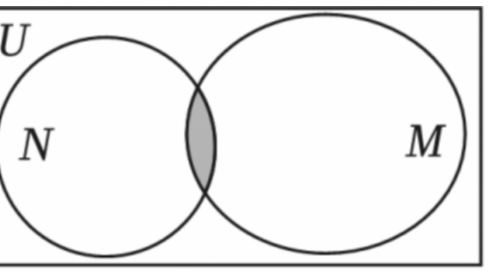
\includegraphics[width=0.30\textwidth]{figures/gao87_q14_venn.png}
\end{center}

\keepwithprev
A. $3$ 个\qquad B. $2$ 个\qquad C. $1$ 个\qquad D. 无穷多个

\ifanswer
\solbegin
\step{阴影部分所示的集合为 $M\cap N$，}
\step{$M=\{x\mid-1\leqslant x\leqslant3\}$，在此范围内的奇数有 $1$ 和 $3$，}
\step{所以集合 $M\cap N=\{1,3\}$ 共有 $2$ 个元素，故选 $B$.}
\solend
\fi

\item 已知实数 $a,b,c$ 满足 $a>b$，则下列不等式成立的是\mbox{（\quad）}

\keepwithprev
A. $-\dfrac1a<\dfrac1b$\qquad B. $a^2>b^2$\qquad C. $a\lvert c\rvert>b\lvert c\rvert$\qquad D. $\dfrac a{c^2+1}>\dfrac b{c^2+1}$

\ifanswer
\solbegin
\step{若 $a=1,b=-1$，则 $-1=-\dfrac1a=\dfrac1b=1$，$a^2=b^2=1$，则 AB 错误；}
\step{若 $a>b,c=0$，则 $a\lvert c\rvert=b\lvert c\rvert=0$，则 C 错误；}
\step{因为 $c^2+1\geqslant1$，所以 $0<\dfrac1{c^2+1}\leqslant1$，又 $a>b$，所以 $\dfrac a{c^2+1}>\dfrac b{c^2+1}$，}
\step{则 D 正确.}
\step{故选 $D$.}
\solend
\fi

\item 设集合 $P_1=\{x\mid x^2+ax+1>0\}$，$P_2=\{x\mid x^2+ax+2>0\}$，$Q_1=\{x\mid x^2+x+b>0\}$，
$Q_2=\{x\mid x^2+2x+b>0\}$，其中 $a$、$b\in\R$，下列说法中正确的是\mbox{（\quad）}

\keepwithprev
A. 对任意 $a$，$P_1$ 是 $P_2$ 的子集，对任意 $b$，$Q_1$ 不是 $Q_2$ 的子集

B. 对任意 $a$，$P_1$ 是 $P_2$ 的子集，存在 $b$，使得 $Q_1$ 是 $Q_2$ 的子集

C. 存在 $a$，使得 $P_1$ 不是 $P_2$ 的子集，对任意 $b$，$Q_1$ 不是 $Q_2$ 的子集

D. 存在 $a$，使得 $P_1$ 不是 $P_2$ 的子集，存在 $b$，使得 $Q_1$ 是 $Q_2$ 的子集

\ifanswer
\solbegin
\step{对于集合 $P_1=\{x\mid x^2+ax+1>0\}$，$P_2=\{x\mid x^2+ax+2>0\}$，}
\step{得当 $m\in P_1$ 时，即 $m^2+am+1>0$，得 $m^2+am+2>0$，}
\step{即有 $m\in P_2$，得对任意 $a$，$P_1$ 是 $P_2$ 的子集，}
\step{对于集合 $Q_1=\{x\mid x^2+x+b>0\}$，$Q_2=\{x\mid x^2+2x+b>0\}$，}
\step{当 $b=6$ 时，$Q_1=\{x\mid x^2+x+6>0\}=\R$，$Q_2=\{x\mid x^2+2x+6>0\}=\R$，}
\step{得 $Q_1$ 是 $Q_2$ 的子集，}
\step{当 $b=1$ 时，$Q_1=\{x\mid x^2+x+1>0\}=\R$，}
\step{$Q_2=\{x\mid x^2+2x+1>0\}=\{x\mid x\neq-1\}$，得 $Q_1$ 不是 $Q_2$ 的子集，}
\step{所以存在 $b$，使得 $Q_1$ 是 $Q_2$ 的子集，故选 $B$.}
\solend
\fi

\end{enumerate}

\bigsec{三、解答题}

\begin{enumerate}
\setcounter{enumi}{16}

\item 设 $m$ 为实数，求关于 $x$ 与 $y$ 的二元一次方程组 $\begin{cases}y=x+m\\ mx-y=4\end{cases}$ 的解集.

\ansspace*[8]

\ifanswer
\solbegin
\step{消去 $y$ 得 $(m-1)x=m+4$，}
\step{当 $m-1=0$，即 $m=1$ 时，$0=5$ 不成立，则 $x$ 无解，原方程组的解集为 $\varnothing$；}
\step{当 $m-1\neq0$，即 $m\neq1$ 时，则 $x=\dfrac{m+4}{m-1}$，$y=\dfrac{m+4}{m-1}+m=\dfrac{m^2+4}{m-1}$，}
\step{原方程组的解集为 $\left\{\left(\dfrac{m+4}{m-1},\dfrac{m^2+4}{m-1}\right)\right\}$.}
\step{综上所述，当 $m=1$ 时，方程组的解集为 $\varnothing$；}
\step{当 $m\neq1$ 时，方程组的解集为 $\left\{\left(\dfrac{m+4}{m-1},\dfrac{m^2+4}{m-1}\right)\right\}$.}
\solend
\fi

\item 设 $x<y<0$，试比较 $(x^2+y^2)(x-y)$ 与 $(x^2-y^2)(x+y)$ 的大小.

\ansspace*[9]

\ifanswer
\solbegin
\step{$(x^2+y^2)(x-y)-(x^2-y^2)(x+y)=(x-y)[x^2+y^2-(x+y)^2]=-2xy(x-y)$，}
\step{因为 $x<y<0$，所以 $xy>0$，$x-y<0$，所以 $-2xy(x-y)>0$，}
\step{即 $(x^2+y^2)(x-y)>(x^2-y^2)(x+y)$.}
\solend
\fi

\item 已知全集 $U=\R$，集合 $A=\left\{x\left|\dfrac{2+x}{3-x}>0\right.\right\}$，集合 $B=\{x\mid\lvert x-2\rvert>3\}$.

（1）求 $A\cup B$、$\overline A\cap B$.

（2）若集合 $C=\{x\mid x\leqslant a\}$，且 $A\cap C=A$，求实数 $a$ 的范围.

\ansspace*[10]

\ifanswer
\solbegin
\stepm{（1）}{由 $\lvert x-2\rvert>3$ 得 $x-2>3$ 或 $x-2<-3$，即 $x<-1$ 或 $x>5$，}
\step{所以 $B=(-\infty,-1)\cup(5,+\infty)$，}
\step{$A=\left\{x\left|\dfrac{2+x}{3-x}>0\right.\right\}=\{x\mid(2+x)(3-x)>0\}=(-2,3)$，}
\step{所以 $A\cup b=(-\infty,3)\cup(5m+\infty)$，}
\step{$\overline A=(-\infty,-2]\cup[3,+\infty)$，$\overline A\cap B=(-\infty,-2]\cup(5,+\infty)$.}
\stepm{（2）}{因为 $A\cap C=A$，所以 $A\subseteq C$，}
\step{因为 $A=(-2,3)$，所以实数 $a$ 的取值范围为 $\{a\mid a\geqslant3\}$.}
\solend
\fi

\item 已知函数 $f(x)=ax^2+4x+b\,(a<0,a,b\in\R)$，设关于 $x$ 的方程 $f(x)=0$ 的两实根为 $x_1$、
$x_2$，方程 $f(x)=x$ 的两实根为 $\alpha,\beta$.

（1）不等式 $f(x)<0$ 的解集是 $(-\infty,-3)\cup(5,+\infty)$，求不等式 $bx^2-ax-4<0$ 的解集；

（2）若 $a,b$ 均为负整数，且 $\lvert\alpha-\beta\rvert=1$，求 $f(x)$ 的解析式.

\ansspace*[12]

\ifanswer
\solbegin
\stepm{（1）}{$ax^2+4x+b<0$ 的解集为 $(-\infty,-3)\cup(5,+\infty)$，}
\step{所以 $-3,5$ 是方程 $ax^2+4x+b=0$ 的两根，所以 $\begin{cases}-3+5=-\dfrac4a\\ -3\times5=\dfrac ba\end{cases}\Rightarrow\begin{cases}a=-2\\ b=30\end{cases}$，}
\step{所以 $bx^2-ax-4<0$ 为 $30x^2+2x-4<0\Rightarrow15x^2+x-2<0$，}
\step{所以 $(3x-1)(5x+2)<0\Rightarrow-\dfrac25<x<\dfrac13$，}
\step{所以所求不等式的解集为 $\left\{x\left|-\dfrac25<x<\dfrac13\right.\right\}$.}
\stepm{（2）}{由题意得 $f(x)=ax^2+4x+b\,(a<0,a,b\in\R)$ 有两个不等实根为 $\alpha$、$\beta$，}
\step{所以 $\Delta=9-4ab>0$，$\alpha+\beta=-\dfrac3a$，$\alpha\beta=\dfrac ba$.}
\step{由 $\lvert\alpha-\beta\rvert=1$ 得 $(\alpha-\beta)^2=1$，即 $(\alpha+\beta)^2-4\alpha\beta=\dfrac9{a^2}-\dfrac{4b}a=1$，}
\step{所以 $9-4ab=a^2$，即 $a^2+4ab=9\,(a<0,a,b\in\R)$.}
\step{因为 $a,b$ 均为负整数，}
\step{所以 $\begin{cases}a=-1\\ a+4b=-9\end{cases}$ 或 $\begin{cases}a=-9\\ a+4b=-1\end{cases}$ 或 $\begin{cases}a=-3\\ a+4b=-3\end{cases}$，}
\step{显然后两种情况不合题意，应舍去，从而有 $\begin{cases}a=-1\\ a+4b=-9\end{cases}$，解得 $a=-1$，$b=-2$.}
\step{故所求函数解析式为 $f(x)=-x^2+4x-2$.}
\solend
\fi

\item 已知集合 $A=\{x\mid x=m^2+n^2,m\in\Z,n\in\Z\}$.

（1）判断 $2,5,25$ 是否属于集合 $A$；

（2）若正整数 $y$ 能表示为某个整数的平方，$z\in A$，证明：$yz\in A$；

（3）若集合 $B=\{x\mid x=4k+3,k\in\Z\}$，证明：$A\cap B=\varnothing$.

\ansspace*[14]

\ifanswer
\solbegin
\stepm{（1）}{由 $2=1^2+1^2$，$5=1^2+2^2$，$25=3^2+4^2$ 得 $2,5,25$ 属于集合 $A$；}
\stepm{（2）}{设 $y=a^2\,(a\in\Z)$，由 $z\in A$，设 $z=b^2+c^2\,(b\in\Z,c\in\Z)$，}
\step{则 $yz=a^2(b^2+c^2)=(ab)^2+(ac)^2$，}
\step{因为 $a\in\Z$，$b\in\Z$，$c\in\Z$，所以 $ab\in\Z$，$ac\in\Z$，所以 $yz\in A$；}
\stepm{（3）}{①当 $m$、$n$ 都为偶数时，设 $m=2k_1\,(k_1\in\Z)$，$n=2k_2\,(k_2\in\Z)$，}
\step{则 $x=m^2+n^2=4k_1^2+4k_2^2=4(k_1^2+k_2^2)$，此时 $x$ 为 $4$ 的倍数，}
\step{因为偶数 $\notin B$，所以 $A\cap B=\varnothing$；}
\step{②当 $m$、$n$ 都为奇数时，设 $m=2k_1+1\,(k_1\in\Z)$，$n=2k_2+1\,(k_2\in\Z)$，}
\step{则 $x=m^2+n^2=(2k_1+1)^2+(2k_2+1)^2=4(k_1^2+k_2^2+k_1+k_2)+2$，}
\step{此时 $x$ 为 $2$ 的倍数，因为偶数 $\notin B$，所以 $A\cap B=\varnothing$；}
\step{③当 $m$、$n$ 一奇一偶时，设 $m=2k_1+1\,(k_1\in\Z)$，$n=2k_2\,(k_2\in\Z)$，}
\step{则 $x=m^2+n^2=(2k_1+1)^2+(2k_2)^2=4(k_1^2+k_2^2+k_1)+1$，}
\step{此时 $x$ 被 $4$ 除余 $1$，而 $B$ 中元素被 $4$ 除余 $3$，此时 $A\cap B=\varnothing$.}
\step{综上，$A\cap B=\varnothing$.}
\solend
\fi

\end{enumerate}

\end{document}
"
%
% 原始材料：微信公众号“魔都数学加油站”文章，连载“27学年高一87”；
% 原文标题“27学年高一87——2026-2027年上海市五十四中学高一上10月月考”；
% 原文链接：https://mp.weixin.qq.com/s/pqPpSGQt0AhydcpaB8uEkQ。
% 页面标注发布时间 2026-10-27 17:43（上海）。
% 正文为 7 张 PNG 页（`原图/高一87_五十四中学_10月月考/01..07.png`），
% 尺寸混排（第 1、2 页为 4762×6735，第 3—7 页为 2560×3620），均按页序读取。
%
% 篇幅与题号：原卷自第 3 题起编号（第 1、2 题不在原文内）。填空题 3—12（10 题）、
% 选择题 13—16（4 题）、解答题 17—21（5 题），共 19 题。
%
% 讲评版：第 3、5、6 题只印【答案】（“$x\leqslant1$ 且 $y\leqslant1$”“$\{(2,6),(6,2)\}$”
% “$(-1,3]$”），本稿只给 \ans{}；其余 16 题印【解析】，其中选择题答案在解析末句
% “故选 A／B／D／B”。第 14 题题干带一幅韦恩图（裁自第 3 页原图、去粉色水印后转灰度），
% 三版都出。
%
% 副标题：原卷未印副标题。本稿按内容标作“集合与常用逻辑用语、不等式”。
%
% 原卷笔误/存疑（均照录未改，正文对应处另有 % 注）：
%   ① 第 19 题 (1) 解析作“所以 $A\cup b=(-\infty,3)\cup(5m+\infty)$”，两处均系排印错：
%      按上下文应为“$A\cup B=(-\infty,3)\cup(5,+\infty)$”（同页下一行 $\overline A\cap B$
%      的端点 $5$、$+\infty$ 也印证这一点）。原卷印作 $b$ 与 $5m+\infty$，照录未改。
%
% 与原卷的排版差异：
%   ① 原卷每题下直接印【答案】/【解析】，本稿按全稿惯例将答案与解析置于答案版；
%   ② 原卷未印副标题，本稿补出；填空横线统一排 \blankline[4.4em]；
%   ③ 原卷数集记号排斜体 $R$、$Z$、$N$，本稿按全稿惯例改用 $\R$、$\Z$、$\N$；
%   ④ 第 17—21 题的子问用行内“（1）（2）（3）”段，解析中的子问标号用 \stepm；
%   ⑤ 解答题按惯例加 \ansspace；选择题括号排 \mbox{（\quad）}。
%
% 行数核对：逐题数 \step/\stepm 条数，合计 86 条（Q4：1；Q7：4；Q8：2；Q9：2；Q10：3；
% Q11：9；Q12：3；Q13：2；Q14：3；Q15：5；Q16：9；Q17：6；Q18：3；Q19：7；Q20：13；
% Q21：14）；第 3、5、6 题只印【答案】，提 \ans{}，不计入 \step 账。原卷解析的换行
% 按语意合并，未逐行强拆。
%
\documentclass[a4paper,11pt]{article}
\usepackage{common}

\begin{document}

\examtitlest[7]{2026--2027 年五十四中学高一上 10 月月考}{集合与常用逻辑用语、不等式}

\bigsec{一、填空题}

\begin{enumerate}
\setcounter{enumi}{2}

\item “$x>1$ 或 $y>1$”的否定形式为\blankline[4.4em].

\ifanswer
\ans{$x\leqslant1$ 且 $y\leqslant1$}
\fi

\item 已知 $1<a<2$，$-3<b<3$，则 $a+b$ 的取值范围是\blankline[4.4em].

\ifanswer
\solbegin
\step{由不等式的可加性得 $-2<a+b<5$，故 $a+b$ 的取值范围是 $(-2,5)$.}
\solend
\fi

\item 方程组 $\begin{cases}x+y=8\\ xy=12\end{cases}$ 的解集为\blankline[4.4em].

\ifanswer
\ans{$\{(2,6),(6,2)\}$}
\fi

\item 不等式 $\dfrac{x-3}{x+1}\leqslant0$ 解集为\blankline[4.4em].

\ifanswer
\ans{$(-1,3]$}
\fi

\item 已知集合 $A=\{x\mid y=\sqrt{x+1}\}$，$B=\{y\mid y=x^2+5\}$，则 $A\cup B=\blankline[4.4em]$.

\ifanswer
\solbegin
\step{对于函数 $y=\sqrt{x+1}$，则 $x+1\geqslant0$，解得 $x\geqslant-1$，}
\step{所以 $A=\{x\mid y=\sqrt{x+1}\}=\{x\mid x\geqslant-1\}$，}
\step{因为 $x^2\geqslant0$，所以 $y=x^2+5\geqslant5$，所以 $B=\{y\mid y=x^2+5\}=\{y\mid y\geqslant5\}$，}
\step{所以 $A\cup B=\{x\mid x\geqslant-1\}$.}
\solend
\fi

\item 已知关于 $x$ 的不等式 $\lvert x+a\rvert<b$ 的解集为 $\{x\mid2<x<4\}$，则 $a+b$ 的值是\blankline[4.4em].

\ifanswer
\solbegin
\step{由 $\lvert x+a\rvert<b$，得 $-b-a<x<b-a$，则 $\begin{cases}-b-a=2\\ b-a=4\end{cases}$，解得 $a=-3$，$b=1$，}
\step{所以 $a+b=-2$.}
\solend
\fi

\item 已知一元二次方程 $x^2-2mx+m-1=0$ 的两实根为 $x_1,x_2$，且 $x_1^2+x_2^2=4$，则实数 $m$ 的值
是\blankline[4.4em].

\ifanswer
\solbegin
\step{由题意得 $x_1+x_2=2m$，$x_1x_2=m-1$，}
\step{所以 $x_1^2+x_2^2=(x_1+x_2)^2-2x_1x_2=4m^2-2m+2=4$，解得 $m=1$ 或 $m=-\dfrac12$.}
\solend
\fi

\item 已知集合 $A=\{x\mid x^2-x-6=0\}$，$B=\{y\mid ay-1=0\}$，若 $A\cap B=B$，则实数
$a=\blankline[4.4em]$.

\ifanswer
\solbegin
\step{$A=\{-2,3\}$，由 $A\cap B=B$，得 $B\subseteq A$，而 $B=\{y\mid ay-1=0\}$，}
\step{则当 $B=\varnothing$ 时，$a=0$；当 $B=\{-2\}$ 时，$-2a-1=0$，解得 $a=-\dfrac12$；}
\step{当 $B=\{3\}$ 时，$3a-1=0$，解得 $a=\dfrac13$，所以实数 $a$ 的值为 $-\dfrac12$ 或 $0$ 或 $\dfrac13$.}
\solend
\fi

\item 已知集合 $A=\{x\mid(m-1)x^2+(m-1)x+2\leqslant0,x\in\R\}$，$B=\left\{x\left|\dfrac{2x-1}{x^2+x+1}>1,x\in\R\right.\right\}$，
且 $A\cap B=A$，则实数 $m$ 的取值范围是\blankline[4.4em].

\ifanswer
\solbegin
\step{因为 $\dfrac{2x-1}{x^2+x+1}>1$，所以 $x^2-x+2<0$，显然不等式无解，}
\step{所以 $B=\left\{x\left|\dfrac{2x-1}{x^2+x+1}>1,x\in\R\right.\right\}=\varnothing$，而 $A\cap B=A$，则 $A=\varnothing$，}
\step{①当 $m=1$ 时，$2\leqslant0$ 不成立，此时 $A=\varnothing$，}
\step{②当 $m<1$ 时，$m-1<0$，函数 $y=(m-1)x^2+(m-1)x+2$，开口向下，}
\step{不等式 $(m-1)x^2+(m-1)x+2\leqslant0$ 有解，$A\neq\varnothing$，}
\step{③当 $m>1$ 时，函数 $y=(m-1)x^2+(m-1)x+2$，开口向上，}
\step{若不等式 $(m-1)x^2+(m-1)x+2\leqslant0$ 无解，}
\step{只需 $\Delta=(m-1)^2-8(m-1)<0$，解得 $1<m<9$，}
\step{综上，$m$ 的取值范围是 $[1,9]$.}
\solend
\fi

\item 设 $A$ 是整数集的一个非空子集，对于 $k\in A$，如果 $k-1\notin A$ 且 $k+1\notin A$，那么 $k$ 是 $A$
的一个“孤立元”. 给定 $S=\{1,2,3,4,5,6,7,8\}$，由 $S$ 的 $3$ 个元素构成的所有集合中，不含
“孤立元”的集合共有\blankline[3.6em]个.

\ifanswer
\solbegin
\step{由题意得，“孤立元”即为在集合中无与之相邻的元素，}
\step{满足条件的集合有 $\{1,2,3\},\{2,3,4\},\{3,4,5\},\{4,5,6\},\{5,6,7\},\{6,7,8\}$，}
\step{共 $6$ 个集合.}
\solend
\fi

\end{enumerate}

\bigsec{二、选择题}

\begin{enumerate}
\setcounter{enumi}{12}

\item “$m=2$”是“$m^2=4$”的\mbox{（\quad）}条件.

\keepwithprev
A. 充分非必要条件\qquad B. 必要非充分条件

C. 充要条件\qquad D. 既非充分又非必要条件

\ifanswer
\solbegin
\step{由 $m^2=4$，解得 $m=\pm2$，故“$m=2$”是“$m^2=4$”的充分不必要条件，}
\step{故选 $A$.}
\solend
\fi

\item 已知全集 $U=\R$，集合 $M=\{x\mid\lvert x-1\rvert\leqslant2\}$ 和 $N=\{x\mid x=2k-1,k\in\Z\}$ 的关系
的韦恩（$Venn$）图如图所示，则阴影部分所示的集合的元素共有\mbox{（\quad）}

\begin{center}
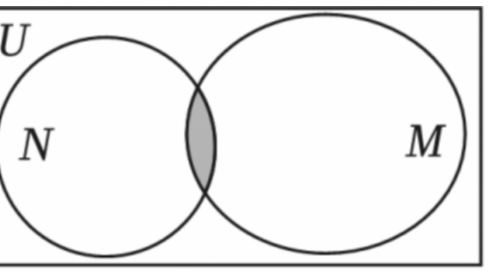
\includegraphics[width=0.30\textwidth]{figures/gao87_q14_venn.png}
\end{center}

\keepwithprev
A. $3$ 个\qquad B. $2$ 个\qquad C. $1$ 个\qquad D. 无穷多个

\ifanswer
\solbegin
\step{阴影部分所示的集合为 $M\cap N$，}
\step{$M=\{x\mid-1\leqslant x\leqslant3\}$，在此范围内的奇数有 $1$ 和 $3$，}
\step{所以集合 $M\cap N=\{1,3\}$ 共有 $2$ 个元素，故选 $B$.}
\solend
\fi

\item 已知实数 $a,b,c$ 满足 $a>b$，则下列不等式成立的是\mbox{（\quad）}

\keepwithprev
A. $-\dfrac1a<\dfrac1b$\qquad B. $a^2>b^2$\qquad C. $a\lvert c\rvert>b\lvert c\rvert$\qquad D. $\dfrac a{c^2+1}>\dfrac b{c^2+1}$

\ifanswer
\solbegin
\step{若 $a=1,b=-1$，则 $-1=-\dfrac1a=\dfrac1b=1$，$a^2=b^2=1$，则 AB 错误；}
\step{若 $a>b,c=0$，则 $a\lvert c\rvert=b\lvert c\rvert=0$，则 C 错误；}
\step{因为 $c^2+1\geqslant1$，所以 $0<\dfrac1{c^2+1}\leqslant1$，又 $a>b$，所以 $\dfrac a{c^2+1}>\dfrac b{c^2+1}$，}
\step{则 D 正确.}
\step{故选 $D$.}
\solend
\fi

\item 设集合 $P_1=\{x\mid x^2+ax+1>0\}$，$P_2=\{x\mid x^2+ax+2>0\}$，$Q_1=\{x\mid x^2+x+b>0\}$，
$Q_2=\{x\mid x^2+2x+b>0\}$，其中 $a$、$b\in\R$，下列说法中正确的是\mbox{（\quad）}

\keepwithprev
A. 对任意 $a$，$P_1$ 是 $P_2$ 的子集，对任意 $b$，$Q_1$ 不是 $Q_2$ 的子集

B. 对任意 $a$，$P_1$ 是 $P_2$ 的子集，存在 $b$，使得 $Q_1$ 是 $Q_2$ 的子集

C. 存在 $a$，使得 $P_1$ 不是 $P_2$ 的子集，对任意 $b$，$Q_1$ 不是 $Q_2$ 的子集

D. 存在 $a$，使得 $P_1$ 不是 $P_2$ 的子集，存在 $b$，使得 $Q_1$ 是 $Q_2$ 的子集

\ifanswer
\solbegin
\step{对于集合 $P_1=\{x\mid x^2+ax+1>0\}$，$P_2=\{x\mid x^2+ax+2>0\}$，}
\step{得当 $m\in P_1$ 时，即 $m^2+am+1>0$，得 $m^2+am+2>0$，}
\step{即有 $m\in P_2$，得对任意 $a$，$P_1$ 是 $P_2$ 的子集，}
\step{对于集合 $Q_1=\{x\mid x^2+x+b>0\}$，$Q_2=\{x\mid x^2+2x+b>0\}$，}
\step{当 $b=6$ 时，$Q_1=\{x\mid x^2+x+6>0\}=\R$，$Q_2=\{x\mid x^2+2x+6>0\}=\R$，}
\step{得 $Q_1$ 是 $Q_2$ 的子集，}
\step{当 $b=1$ 时，$Q_1=\{x\mid x^2+x+1>0\}=\R$，}
\step{$Q_2=\{x\mid x^2+2x+1>0\}=\{x\mid x\neq-1\}$，得 $Q_1$ 不是 $Q_2$ 的子集，}
\step{所以存在 $b$，使得 $Q_1$ 是 $Q_2$ 的子集，故选 $B$.}
\solend
\fi

\end{enumerate}

\bigsec{三、解答题}

\begin{enumerate}
\setcounter{enumi}{16}

\item 设 $m$ 为实数，求关于 $x$ 与 $y$ 的二元一次方程组 $\begin{cases}y=x+m\\ mx-y=4\end{cases}$ 的解集.

\ansspace*[8]

\ifanswer
\solbegin
\step{消去 $y$ 得 $(m-1)x=m+4$，}
\step{当 $m-1=0$，即 $m=1$ 时，$0=5$ 不成立，则 $x$ 无解，原方程组的解集为 $\varnothing$；}
\step{当 $m-1\neq0$，即 $m\neq1$ 时，则 $x=\dfrac{m+4}{m-1}$，$y=\dfrac{m+4}{m-1}+m=\dfrac{m^2+4}{m-1}$，}
\step{原方程组的解集为 $\left\{\left(\dfrac{m+4}{m-1},\dfrac{m^2+4}{m-1}\right)\right\}$.}
\step{综上所述，当 $m=1$ 时，方程组的解集为 $\varnothing$；}
\step{当 $m\neq1$ 时，方程组的解集为 $\left\{\left(\dfrac{m+4}{m-1},\dfrac{m^2+4}{m-1}\right)\right\}$.}
\solend
\fi

\item 设 $x<y<0$，试比较 $(x^2+y^2)(x-y)$ 与 $(x^2-y^2)(x+y)$ 的大小.

\ansspace*[9]

\ifanswer
\solbegin
\step{$(x^2+y^2)(x-y)-(x^2-y^2)(x+y)=(x-y)[x^2+y^2-(x+y)^2]=-2xy(x-y)$，}
\step{因为 $x<y<0$，所以 $xy>0$，$x-y<0$，所以 $-2xy(x-y)>0$，}
\step{即 $(x^2+y^2)(x-y)>(x^2-y^2)(x+y)$.}
\solend
\fi

\item 已知全集 $U=\R$，集合 $A=\left\{x\left|\dfrac{2+x}{3-x}>0\right.\right\}$，集合 $B=\{x\mid\lvert x-2\rvert>3\}$.

（1）求 $A\cup B$、$\overline A\cap B$.

（2）若集合 $C=\{x\mid x\leqslant a\}$，且 $A\cap C=A$，求实数 $a$ 的范围.

\ansspace*[10]

\ifanswer
\solbegin
\stepm{（1）}{由 $\lvert x-2\rvert>3$ 得 $x-2>3$ 或 $x-2<-3$，即 $x<-1$ 或 $x>5$，}
\step{所以 $B=(-\infty,-1)\cup(5,+\infty)$，}
\step{$A=\left\{x\left|\dfrac{2+x}{3-x}>0\right.\right\}=\{x\mid(2+x)(3-x)>0\}=(-2,3)$，}
\step{所以 $A\cup b=(-\infty,3)\cup(5m+\infty)$，}
\step{$\overline A=(-\infty,-2]\cup[3,+\infty)$，$\overline A\cap B=(-\infty,-2]\cup(5,+\infty)$.}
\stepm{（2）}{因为 $A\cap C=A$，所以 $A\subseteq C$，}
\step{因为 $A=(-2,3)$，所以实数 $a$ 的取值范围为 $\{a\mid a\geqslant3\}$.}
\solend
\fi

\item 已知函数 $f(x)=ax^2+4x+b\,(a<0,a,b\in\R)$，设关于 $x$ 的方程 $f(x)=0$ 的两实根为 $x_1$、
$x_2$，方程 $f(x)=x$ 的两实根为 $\alpha,\beta$.

（1）不等式 $f(x)<0$ 的解集是 $(-\infty,-3)\cup(5,+\infty)$，求不等式 $bx^2-ax-4<0$ 的解集；

（2）若 $a,b$ 均为负整数，且 $\lvert\alpha-\beta\rvert=1$，求 $f(x)$ 的解析式.

\ansspace*[12]

\ifanswer
\solbegin
\stepm{（1）}{$ax^2+4x+b<0$ 的解集为 $(-\infty,-3)\cup(5,+\infty)$，}
\step{所以 $-3,5$ 是方程 $ax^2+4x+b=0$ 的两根，所以 $\begin{cases}-3+5=-\dfrac4a\\ -3\times5=\dfrac ba\end{cases}\Rightarrow\begin{cases}a=-2\\ b=30\end{cases}$，}
\step{所以 $bx^2-ax-4<0$ 为 $30x^2+2x-4<0\Rightarrow15x^2+x-2<0$，}
\step{所以 $(3x-1)(5x+2)<0\Rightarrow-\dfrac25<x<\dfrac13$，}
\step{所以所求不等式的解集为 $\left\{x\left|-\dfrac25<x<\dfrac13\right.\right\}$.}
\stepm{（2）}{由题意得 $f(x)=ax^2+4x+b\,(a<0,a,b\in\R)$ 有两个不等实根为 $\alpha$、$\beta$，}
\step{所以 $\Delta=9-4ab>0$，$\alpha+\beta=-\dfrac3a$，$\alpha\beta=\dfrac ba$.}
\step{由 $\lvert\alpha-\beta\rvert=1$ 得 $(\alpha-\beta)^2=1$，即 $(\alpha+\beta)^2-4\alpha\beta=\dfrac9{a^2}-\dfrac{4b}a=1$，}
\step{所以 $9-4ab=a^2$，即 $a^2+4ab=9\,(a<0,a,b\in\R)$.}
\step{因为 $a,b$ 均为负整数，}
\step{所以 $\begin{cases}a=-1\\ a+4b=-9\end{cases}$ 或 $\begin{cases}a=-9\\ a+4b=-1\end{cases}$ 或 $\begin{cases}a=-3\\ a+4b=-3\end{cases}$，}
\step{显然后两种情况不合题意，应舍去，从而有 $\begin{cases}a=-1\\ a+4b=-9\end{cases}$，解得 $a=-1$，$b=-2$.}
\step{故所求函数解析式为 $f(x)=-x^2+4x-2$.}
\solend
\fi

\item 已知集合 $A=\{x\mid x=m^2+n^2,m\in\Z,n\in\Z\}$.

（1）判断 $2,5,25$ 是否属于集合 $A$；

（2）若正整数 $y$ 能表示为某个整数的平方，$z\in A$，证明：$yz\in A$；

（3）若集合 $B=\{x\mid x=4k+3,k\in\Z\}$，证明：$A\cap B=\varnothing$.

\ansspace*[14]

\ifanswer
\solbegin
\stepm{（1）}{由 $2=1^2+1^2$，$5=1^2+2^2$，$25=3^2+4^2$ 得 $2,5,25$ 属于集合 $A$；}
\stepm{（2）}{设 $y=a^2\,(a\in\Z)$，由 $z\in A$，设 $z=b^2+c^2\,(b\in\Z,c\in\Z)$，}
\step{则 $yz=a^2(b^2+c^2)=(ab)^2+(ac)^2$，}
\step{因为 $a\in\Z$，$b\in\Z$，$c\in\Z$，所以 $ab\in\Z$，$ac\in\Z$，所以 $yz\in A$；}
\stepm{（3）}{①当 $m$、$n$ 都为偶数时，设 $m=2k_1\,(k_1\in\Z)$，$n=2k_2\,(k_2\in\Z)$，}
\step{则 $x=m^2+n^2=4k_1^2+4k_2^2=4(k_1^2+k_2^2)$，此时 $x$ 为 $4$ 的倍数，}
\step{因为偶数 $\notin B$，所以 $A\cap B=\varnothing$；}
\step{②当 $m$、$n$ 都为奇数时，设 $m=2k_1+1\,(k_1\in\Z)$，$n=2k_2+1\,(k_2\in\Z)$，}
\step{则 $x=m^2+n^2=(2k_1+1)^2+(2k_2+1)^2=4(k_1^2+k_2^2+k_1+k_2)+2$，}
\step{此时 $x$ 为 $2$ 的倍数，因为偶数 $\notin B$，所以 $A\cap B=\varnothing$；}
\step{③当 $m$、$n$ 一奇一偶时，设 $m=2k_1+1\,(k_1\in\Z)$，$n=2k_2\,(k_2\in\Z)$，}
\step{则 $x=m^2+n^2=(2k_1+1)^2+(2k_2)^2=4(k_1^2+k_2^2+k_1)+1$，}
\step{此时 $x$ 被 $4$ 除余 $1$，而 $B$ 中元素被 $4$ 除余 $3$，此时 $A\cap B=\varnothing$.}
\step{综上，$A\cap B=\varnothing$.}
\solend
\fi

\end{enumerate}

\end{document}
"
%
% 原始材料：微信公众号“魔都数学加油站”文章，连载“27学年高一87”；
% 原文标题“27学年高一87——2026-2027年上海市五十四中学高一上10月月考”；
% 原文链接：https://mp.weixin.qq.com/s/pqPpSGQt0AhydcpaB8uEkQ。
% 页面标注发布时间 2026-10-27 17:43（上海）。
% 正文为 7 张 PNG 页（`原图/高一87_五十四中学_10月月考/01..07.png`），
% 尺寸混排（第 1、2 页为 4762×6735，第 3—7 页为 2560×3620），均按页序读取。
%
% 篇幅与题号：原卷自第 3 题起编号（第 1、2 题不在原文内）。填空题 3—12（10 题）、
% 选择题 13—16（4 题）、解答题 17—21（5 题），共 19 题。
%
% 讲评版：第 3、5、6 题只印【答案】（“$x\leqslant1$ 且 $y\leqslant1$”“$\{(2,6),(6,2)\}$”
% “$(-1,3]$”），本稿只给 \ans{}；其余 16 题印【解析】，其中选择题答案在解析末句
% “故选 A／B／D／B”。第 14 题题干带一幅韦恩图（裁自第 3 页原图、去粉色水印后转灰度），
% 三版都出。
%
% 副标题：原卷未印副标题。本稿按内容标作“集合与常用逻辑用语、不等式”。
%
% 原卷笔误/存疑（均照录未改，正文对应处另有 % 注）：
%   ① 第 19 题 (1) 解析作“所以 $A\cup b=(-\infty,3)\cup(5m+\infty)$”，两处均系排印错：
%      按上下文应为“$A\cup B=(-\infty,3)\cup(5,+\infty)$”（同页下一行 $\overline A\cap B$
%      的端点 $5$、$+\infty$ 也印证这一点）。原卷印作 $b$ 与 $5m+\infty$，照录未改。
%
% 与原卷的排版差异：
%   ① 原卷每题下直接印【答案】/【解析】，本稿按全稿惯例将答案与解析置于答案版；
%   ② 原卷未印副标题，本稿补出；填空横线统一排 \blankline[4.4em]；
%   ③ 原卷数集记号排斜体 $R$、$Z$、$N$，本稿按全稿惯例改用 $\R$、$\Z$、$\N$；
%   ④ 第 17—21 题的子问用行内“（1）（2）（3）”段，解析中的子问标号用 \stepm；
%   ⑤ 解答题按惯例加 \ansspace；选择题括号排 \mbox{（\quad）}。
%
% 行数核对：逐题数 \step/\stepm 条数，合计 86 条（Q4：1；Q7：4；Q8：2；Q9：2；Q10：3；
% Q11：9；Q12：3；Q13：2；Q14：3；Q15：5；Q16：9；Q17：6；Q18：3；Q19：7；Q20：13；
% Q21：14）；第 3、5、6 题只印【答案】，提 \ans{}，不计入 \step 账。原卷解析的换行
% 按语意合并，未逐行强拆。
%
\documentclass[a4paper,11pt]{article}
\usepackage{common}

\begin{document}

\examtitlest[7]{2026--2027 年五十四中学高一上 10 月月考}{集合与常用逻辑用语、不等式}

\bigsec{一、填空题}

\begin{enumerate}
\setcounter{enumi}{2}

\item “$x>1$ 或 $y>1$”的否定形式为\blankline[4.4em].

\ifanswer
\ans{$x\leqslant1$ 且 $y\leqslant1$}
\fi

\item 已知 $1<a<2$，$-3<b<3$，则 $a+b$ 的取值范围是\blankline[4.4em].

\ifanswer
\solbegin
\step{由不等式的可加性得 $-2<a+b<5$，故 $a+b$ 的取值范围是 $(-2,5)$.}
\solend
\fi

\item 方程组 $\begin{cases}x+y=8\\ xy=12\end{cases}$ 的解集为\blankline[4.4em].

\ifanswer
\ans{$\{(2,6),(6,2)\}$}
\fi

\item 不等式 $\dfrac{x-3}{x+1}\leqslant0$ 解集为\blankline[4.4em].

\ifanswer
\ans{$(-1,3]$}
\fi

\item 已知集合 $A=\{x\mid y=\sqrt{x+1}\}$，$B=\{y\mid y=x^2+5\}$，则 $A\cup B=\blankline[4.4em]$.

\ifanswer
\solbegin
\step{对于函数 $y=\sqrt{x+1}$，则 $x+1\geqslant0$，解得 $x\geqslant-1$，}
\step{所以 $A=\{x\mid y=\sqrt{x+1}\}=\{x\mid x\geqslant-1\}$，}
\step{因为 $x^2\geqslant0$，所以 $y=x^2+5\geqslant5$，所以 $B=\{y\mid y=x^2+5\}=\{y\mid y\geqslant5\}$，}
\step{所以 $A\cup B=\{x\mid x\geqslant-1\}$.}
\solend
\fi

\item 已知关于 $x$ 的不等式 $\lvert x+a\rvert<b$ 的解集为 $\{x\mid2<x<4\}$，则 $a+b$ 的值是\blankline[4.4em].

\ifanswer
\solbegin
\step{由 $\lvert x+a\rvert<b$，得 $-b-a<x<b-a$，则 $\begin{cases}-b-a=2\\ b-a=4\end{cases}$，解得 $a=-3$，$b=1$，}
\step{所以 $a+b=-2$.}
\solend
\fi

\item 已知一元二次方程 $x^2-2mx+m-1=0$ 的两实根为 $x_1,x_2$，且 $x_1^2+x_2^2=4$，则实数 $m$ 的值
是\blankline[4.4em].

\ifanswer
\solbegin
\step{由题意得 $x_1+x_2=2m$，$x_1x_2=m-1$，}
\step{所以 $x_1^2+x_2^2=(x_1+x_2)^2-2x_1x_2=4m^2-2m+2=4$，解得 $m=1$ 或 $m=-\dfrac12$.}
\solend
\fi

\item 已知集合 $A=\{x\mid x^2-x-6=0\}$，$B=\{y\mid ay-1=0\}$，若 $A\cap B=B$，则实数
$a=\blankline[4.4em]$.

\ifanswer
\solbegin
\step{$A=\{-2,3\}$，由 $A\cap B=B$，得 $B\subseteq A$，而 $B=\{y\mid ay-1=0\}$，}
\step{则当 $B=\varnothing$ 时，$a=0$；当 $B=\{-2\}$ 时，$-2a-1=0$，解得 $a=-\dfrac12$；}
\step{当 $B=\{3\}$ 时，$3a-1=0$，解得 $a=\dfrac13$，所以实数 $a$ 的值为 $-\dfrac12$ 或 $0$ 或 $\dfrac13$.}
\solend
\fi

\item 已知集合 $A=\{x\mid(m-1)x^2+(m-1)x+2\leqslant0,x\in\R\}$，$B=\left\{x\left|\dfrac{2x-1}{x^2+x+1}>1,x\in\R\right.\right\}$，
且 $A\cap B=A$，则实数 $m$ 的取值范围是\blankline[4.4em].

\ifanswer
\solbegin
\step{因为 $\dfrac{2x-1}{x^2+x+1}>1$，所以 $x^2-x+2<0$，显然不等式无解，}
\step{所以 $B=\left\{x\left|\dfrac{2x-1}{x^2+x+1}>1,x\in\R\right.\right\}=\varnothing$，而 $A\cap B=A$，则 $A=\varnothing$，}
\step{①当 $m=1$ 时，$2\leqslant0$ 不成立，此时 $A=\varnothing$，}
\step{②当 $m<1$ 时，$m-1<0$，函数 $y=(m-1)x^2+(m-1)x+2$，开口向下，}
\step{不等式 $(m-1)x^2+(m-1)x+2\leqslant0$ 有解，$A\neq\varnothing$，}
\step{③当 $m>1$ 时，函数 $y=(m-1)x^2+(m-1)x+2$，开口向上，}
\step{若不等式 $(m-1)x^2+(m-1)x+2\leqslant0$ 无解，}
\step{只需 $\Delta=(m-1)^2-8(m-1)<0$，解得 $1<m<9$，}
\step{综上，$m$ 的取值范围是 $[1,9]$.}
\solend
\fi

\item 设 $A$ 是整数集的一个非空子集，对于 $k\in A$，如果 $k-1\notin A$ 且 $k+1\notin A$，那么 $k$ 是 $A$
的一个“孤立元”. 给定 $S=\{1,2,3,4,5,6,7,8\}$，由 $S$ 的 $3$ 个元素构成的所有集合中，不含
“孤立元”的集合共有\blankline[3.6em]个.

\ifanswer
\solbegin
\step{由题意得，“孤立元”即为在集合中无与之相邻的元素，}
\step{满足条件的集合有 $\{1,2,3\},\{2,3,4\},\{3,4,5\},\{4,5,6\},\{5,6,7\},\{6,7,8\}$，}
\step{共 $6$ 个集合.}
\solend
\fi

\end{enumerate}

\bigsec{二、选择题}

\begin{enumerate}
\setcounter{enumi}{12}

\item “$m=2$”是“$m^2=4$”的\mbox{（\quad）}条件.

\keepwithprev
A. 充分非必要条件\qquad B. 必要非充分条件

C. 充要条件\qquad D. 既非充分又非必要条件

\ifanswer
\solbegin
\step{由 $m^2=4$，解得 $m=\pm2$，故“$m=2$”是“$m^2=4$”的充分不必要条件，}
\step{故选 $A$.}
\solend
\fi

\item 已知全集 $U=\R$，集合 $M=\{x\mid\lvert x-1\rvert\leqslant2\}$ 和 $N=\{x\mid x=2k-1,k\in\Z\}$ 的关系
的韦恩（$Venn$）图如图所示，则阴影部分所示的集合的元素共有\mbox{（\quad）}

\begin{center}
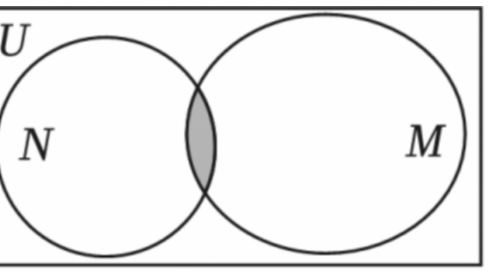
\includegraphics[width=0.30\textwidth]{figures/gao87_q14_venn.png}
\end{center}

\keepwithprev
A. $3$ 个\qquad B. $2$ 个\qquad C. $1$ 个\qquad D. 无穷多个

\ifanswer
\solbegin
\step{阴影部分所示的集合为 $M\cap N$，}
\step{$M=\{x\mid-1\leqslant x\leqslant3\}$，在此范围内的奇数有 $1$ 和 $3$，}
\step{所以集合 $M\cap N=\{1,3\}$ 共有 $2$ 个元素，故选 $B$.}
\solend
\fi

\item 已知实数 $a,b,c$ 满足 $a>b$，则下列不等式成立的是\mbox{（\quad）}

\keepwithprev
A. $-\dfrac1a<\dfrac1b$\qquad B. $a^2>b^2$\qquad C. $a\lvert c\rvert>b\lvert c\rvert$\qquad D. $\dfrac a{c^2+1}>\dfrac b{c^2+1}$

\ifanswer
\solbegin
\step{若 $a=1,b=-1$，则 $-1=-\dfrac1a=\dfrac1b=1$，$a^2=b^2=1$，则 AB 错误；}
\step{若 $a>b,c=0$，则 $a\lvert c\rvert=b\lvert c\rvert=0$，则 C 错误；}
\step{因为 $c^2+1\geqslant1$，所以 $0<\dfrac1{c^2+1}\leqslant1$，又 $a>b$，所以 $\dfrac a{c^2+1}>\dfrac b{c^2+1}$，}
\step{则 D 正确.}
\step{故选 $D$.}
\solend
\fi

\item 设集合 $P_1=\{x\mid x^2+ax+1>0\}$，$P_2=\{x\mid x^2+ax+2>0\}$，$Q_1=\{x\mid x^2+x+b>0\}$，
$Q_2=\{x\mid x^2+2x+b>0\}$，其中 $a$、$b\in\R$，下列说法中正确的是\mbox{（\quad）}

\keepwithprev
A. 对任意 $a$，$P_1$ 是 $P_2$ 的子集，对任意 $b$，$Q_1$ 不是 $Q_2$ 的子集

B. 对任意 $a$，$P_1$ 是 $P_2$ 的子集，存在 $b$，使得 $Q_1$ 是 $Q_2$ 的子集

C. 存在 $a$，使得 $P_1$ 不是 $P_2$ 的子集，对任意 $b$，$Q_1$ 不是 $Q_2$ 的子集

D. 存在 $a$，使得 $P_1$ 不是 $P_2$ 的子集，存在 $b$，使得 $Q_1$ 是 $Q_2$ 的子集

\ifanswer
\solbegin
\step{对于集合 $P_1=\{x\mid x^2+ax+1>0\}$，$P_2=\{x\mid x^2+ax+2>0\}$，}
\step{得当 $m\in P_1$ 时，即 $m^2+am+1>0$，得 $m^2+am+2>0$，}
\step{即有 $m\in P_2$，得对任意 $a$，$P_1$ 是 $P_2$ 的子集，}
\step{对于集合 $Q_1=\{x\mid x^2+x+b>0\}$，$Q_2=\{x\mid x^2+2x+b>0\}$，}
\step{当 $b=6$ 时，$Q_1=\{x\mid x^2+x+6>0\}=\R$，$Q_2=\{x\mid x^2+2x+6>0\}=\R$，}
\step{得 $Q_1$ 是 $Q_2$ 的子集，}
\step{当 $b=1$ 时，$Q_1=\{x\mid x^2+x+1>0\}=\R$，}
\step{$Q_2=\{x\mid x^2+2x+1>0\}=\{x\mid x\neq-1\}$，得 $Q_1$ 不是 $Q_2$ 的子集，}
\step{所以存在 $b$，使得 $Q_1$ 是 $Q_2$ 的子集，故选 $B$.}
\solend
\fi

\end{enumerate}

\bigsec{三、解答题}

\begin{enumerate}
\setcounter{enumi}{16}

\item 设 $m$ 为实数，求关于 $x$ 与 $y$ 的二元一次方程组 $\begin{cases}y=x+m\\ mx-y=4\end{cases}$ 的解集.

\ansspace*[8]

\ifanswer
\solbegin
\step{消去 $y$ 得 $(m-1)x=m+4$，}
\step{当 $m-1=0$，即 $m=1$ 时，$0=5$ 不成立，则 $x$ 无解，原方程组的解集为 $\varnothing$；}
\step{当 $m-1\neq0$，即 $m\neq1$ 时，则 $x=\dfrac{m+4}{m-1}$，$y=\dfrac{m+4}{m-1}+m=\dfrac{m^2+4}{m-1}$，}
\step{原方程组的解集为 $\left\{\left(\dfrac{m+4}{m-1},\dfrac{m^2+4}{m-1}\right)\right\}$.}
\step{综上所述，当 $m=1$ 时，方程组的解集为 $\varnothing$；}
\step{当 $m\neq1$ 时，方程组的解集为 $\left\{\left(\dfrac{m+4}{m-1},\dfrac{m^2+4}{m-1}\right)\right\}$.}
\solend
\fi

\item 设 $x<y<0$，试比较 $(x^2+y^2)(x-y)$ 与 $(x^2-y^2)(x+y)$ 的大小.

\ansspace*[9]

\ifanswer
\solbegin
\step{$(x^2+y^2)(x-y)-(x^2-y^2)(x+y)=(x-y)[x^2+y^2-(x+y)^2]=-2xy(x-y)$，}
\step{因为 $x<y<0$，所以 $xy>0$，$x-y<0$，所以 $-2xy(x-y)>0$，}
\step{即 $(x^2+y^2)(x-y)>(x^2-y^2)(x+y)$.}
\solend
\fi

\item 已知全集 $U=\R$，集合 $A=\left\{x\left|\dfrac{2+x}{3-x}>0\right.\right\}$，集合 $B=\{x\mid\lvert x-2\rvert>3\}$.

（1）求 $A\cup B$、$\overline A\cap B$.

（2）若集合 $C=\{x\mid x\leqslant a\}$，且 $A\cap C=A$，求实数 $a$ 的范围.

\ansspace*[10]

\ifanswer
\solbegin
\stepm{（1）}{由 $\lvert x-2\rvert>3$ 得 $x-2>3$ 或 $x-2<-3$，即 $x<-1$ 或 $x>5$，}
\step{所以 $B=(-\infty,-1)\cup(5,+\infty)$，}
\step{$A=\left\{x\left|\dfrac{2+x}{3-x}>0\right.\right\}=\{x\mid(2+x)(3-x)>0\}=(-2,3)$，}
\step{所以 $A\cup b=(-\infty,3)\cup(5m+\infty)$，}
\step{$\overline A=(-\infty,-2]\cup[3,+\infty)$，$\overline A\cap B=(-\infty,-2]\cup(5,+\infty)$.}
\stepm{（2）}{因为 $A\cap C=A$，所以 $A\subseteq C$，}
\step{因为 $A=(-2,3)$，所以实数 $a$ 的取值范围为 $\{a\mid a\geqslant3\}$.}
\solend
\fi

\item 已知函数 $f(x)=ax^2+4x+b\,(a<0,a,b\in\R)$，设关于 $x$ 的方程 $f(x)=0$ 的两实根为 $x_1$、
$x_2$，方程 $f(x)=x$ 的两实根为 $\alpha,\beta$.

（1）不等式 $f(x)<0$ 的解集是 $(-\infty,-3)\cup(5,+\infty)$，求不等式 $bx^2-ax-4<0$ 的解集；

（2）若 $a,b$ 均为负整数，且 $\lvert\alpha-\beta\rvert=1$，求 $f(x)$ 的解析式.

\ansspace*[12]

\ifanswer
\solbegin
\stepm{（1）}{$ax^2+4x+b<0$ 的解集为 $(-\infty,-3)\cup(5,+\infty)$，}
\step{所以 $-3,5$ 是方程 $ax^2+4x+b=0$ 的两根，所以 $\begin{cases}-3+5=-\dfrac4a\\ -3\times5=\dfrac ba\end{cases}\Rightarrow\begin{cases}a=-2\\ b=30\end{cases}$，}
\step{所以 $bx^2-ax-4<0$ 为 $30x^2+2x-4<0\Rightarrow15x^2+x-2<0$，}
\step{所以 $(3x-1)(5x+2)<0\Rightarrow-\dfrac25<x<\dfrac13$，}
\step{所以所求不等式的解集为 $\left\{x\left|-\dfrac25<x<\dfrac13\right.\right\}$.}
\stepm{（2）}{由题意得 $f(x)=ax^2+4x+b\,(a<0,a,b\in\R)$ 有两个不等实根为 $\alpha$、$\beta$，}
\step{所以 $\Delta=9-4ab>0$，$\alpha+\beta=-\dfrac3a$，$\alpha\beta=\dfrac ba$.}
\step{由 $\lvert\alpha-\beta\rvert=1$ 得 $(\alpha-\beta)^2=1$，即 $(\alpha+\beta)^2-4\alpha\beta=\dfrac9{a^2}-\dfrac{4b}a=1$，}
\step{所以 $9-4ab=a^2$，即 $a^2+4ab=9\,(a<0,a,b\in\R)$.}
\step{因为 $a,b$ 均为负整数，}
\step{所以 $\begin{cases}a=-1\\ a+4b=-9\end{cases}$ 或 $\begin{cases}a=-9\\ a+4b=-1\end{cases}$ 或 $\begin{cases}a=-3\\ a+4b=-3\end{cases}$，}
\step{显然后两种情况不合题意，应舍去，从而有 $\begin{cases}a=-1\\ a+4b=-9\end{cases}$，解得 $a=-1$，$b=-2$.}
\step{故所求函数解析式为 $f(x)=-x^2+4x-2$.}
\solend
\fi

\item 已知集合 $A=\{x\mid x=m^2+n^2,m\in\Z,n\in\Z\}$.

（1）判断 $2,5,25$ 是否属于集合 $A$；

（2）若正整数 $y$ 能表示为某个整数的平方，$z\in A$，证明：$yz\in A$；

（3）若集合 $B=\{x\mid x=4k+3,k\in\Z\}$，证明：$A\cap B=\varnothing$.

\ansspace*[14]

\ifanswer
\solbegin
\stepm{（1）}{由 $2=1^2+1^2$，$5=1^2+2^2$，$25=3^2+4^2$ 得 $2,5,25$ 属于集合 $A$；}
\stepm{（2）}{设 $y=a^2\,(a\in\Z)$，由 $z\in A$，设 $z=b^2+c^2\,(b\in\Z,c\in\Z)$，}
\step{则 $yz=a^2(b^2+c^2)=(ab)^2+(ac)^2$，}
\step{因为 $a\in\Z$，$b\in\Z$，$c\in\Z$，所以 $ab\in\Z$，$ac\in\Z$，所以 $yz\in A$；}
\stepm{（3）}{①当 $m$、$n$ 都为偶数时，设 $m=2k_1\,(k_1\in\Z)$，$n=2k_2\,(k_2\in\Z)$，}
\step{则 $x=m^2+n^2=4k_1^2+4k_2^2=4(k_1^2+k_2^2)$，此时 $x$ 为 $4$ 的倍数，}
\step{因为偶数 $\notin B$，所以 $A\cap B=\varnothing$；}
\step{②当 $m$、$n$ 都为奇数时，设 $m=2k_1+1\,(k_1\in\Z)$，$n=2k_2+1\,(k_2\in\Z)$，}
\step{则 $x=m^2+n^2=(2k_1+1)^2+(2k_2+1)^2=4(k_1^2+k_2^2+k_1+k_2)+2$，}
\step{此时 $x$ 为 $2$ 的倍数，因为偶数 $\notin B$，所以 $A\cap B=\varnothing$；}
\step{③当 $m$、$n$ 一奇一偶时，设 $m=2k_1+1\,(k_1\in\Z)$，$n=2k_2\,(k_2\in\Z)$，}
\step{则 $x=m^2+n^2=(2k_1+1)^2+(2k_2)^2=4(k_1^2+k_2^2+k_1)+1$，}
\step{此时 $x$ 被 $4$ 除余 $1$，而 $B$ 中元素被 $4$ 除余 $3$，此时 $A\cap B=\varnothing$.}
\step{综上，$A\cap B=\varnothing$.}
\solend
\fi

\end{enumerate}

\end{document}
"
% 紧凑版：xelatex "\def\iscompact{1}% 高一87_五十四中学_10月月考.tex
%   —— 高一上数学“2026-2027 年五十四中学高一上 10 月月考”（讲评版）
% 试卷版：xelatex 高一87_五十四中学_10月月考.tex
% 答案版：xelatex "\def\isanswer{1}% 高一87_五十四中学_10月月考.tex
%   —— 高一上数学“2026-2027 年五十四中学高一上 10 月月考”（讲评版）
% 试卷版：xelatex 高一87_五十四中学_10月月考.tex
% 答案版：xelatex "\def\isanswer{1}% 高一87_五十四中学_10月月考.tex
%   —— 高一上数学“2026-2027 年五十四中学高一上 10 月月考”（讲评版）
% 试卷版：xelatex 高一87_五十四中学_10月月考.tex
% 答案版：xelatex "\def\isanswer{1}\input{高一87_五十四中学_10月月考.tex}"
% 紧凑版：xelatex "\def\iscompact{1}\input{高一87_五十四中学_10月月考.tex}"
%
% 原始材料：微信公众号“魔都数学加油站”文章，连载“27学年高一87”；
% 原文标题“27学年高一87——2026-2027年上海市五十四中学高一上10月月考”；
% 原文链接：https://mp.weixin.qq.com/s/pqPpSGQt0AhydcpaB8uEkQ。
% 页面标注发布时间 2026-10-27 17:43（上海）。
% 正文为 7 张 PNG 页（`原图/高一87_五十四中学_10月月考/01..07.png`），
% 尺寸混排（第 1、2 页为 4762×6735，第 3—7 页为 2560×3620），均按页序读取。
%
% 篇幅与题号：原卷自第 3 题起编号（第 1、2 题不在原文内）。填空题 3—12（10 题）、
% 选择题 13—16（4 题）、解答题 17—21（5 题），共 19 题。
%
% 讲评版：第 3、5、6 题只印【答案】（“$x\leqslant1$ 且 $y\leqslant1$”“$\{(2,6),(6,2)\}$”
% “$(-1,3]$”），本稿只给 \ans{}；其余 16 题印【解析】，其中选择题答案在解析末句
% “故选 A／B／D／B”。第 14 题题干带一幅韦恩图（裁自第 3 页原图、去粉色水印后转灰度），
% 三版都出。
%
% 副标题：原卷未印副标题。本稿按内容标作“集合与常用逻辑用语、不等式”。
%
% 原卷笔误/存疑（均照录未改，正文对应处另有 % 注）：
%   ① 第 19 题 (1) 解析作“所以 $A\cup b=(-\infty,3)\cup(5m+\infty)$”，两处均系排印错：
%      按上下文应为“$A\cup B=(-\infty,3)\cup(5,+\infty)$”（同页下一行 $\overline A\cap B$
%      的端点 $5$、$+\infty$ 也印证这一点）。原卷印作 $b$ 与 $5m+\infty$，照录未改。
%
% 与原卷的排版差异：
%   ① 原卷每题下直接印【答案】/【解析】，本稿按全稿惯例将答案与解析置于答案版；
%   ② 原卷未印副标题，本稿补出；填空横线统一排 \blankline[4.4em]；
%   ③ 原卷数集记号排斜体 $R$、$Z$、$N$，本稿按全稿惯例改用 $\R$、$\Z$、$\N$；
%   ④ 第 17—21 题的子问用行内“（1）（2）（3）”段，解析中的子问标号用 \stepm；
%   ⑤ 解答题按惯例加 \ansspace；选择题括号排 \mbox{（\quad）}。
%
% 行数核对：逐题数 \step/\stepm 条数，合计 86 条（Q4：1；Q7：4；Q8：2；Q9：2；Q10：3；
% Q11：9；Q12：3；Q13：2；Q14：3；Q15：5；Q16：9；Q17：6；Q18：3；Q19：7；Q20：13；
% Q21：14）；第 3、5、6 题只印【答案】，提 \ans{}，不计入 \step 账。原卷解析的换行
% 按语意合并，未逐行强拆。
%
\documentclass[a4paper,11pt]{article}
\usepackage{common}

\begin{document}

\examtitlest[7]{2026--2027 年五十四中学高一上 10 月月考}{集合与常用逻辑用语、不等式}

\bigsec{一、填空题}

\begin{enumerate}
\setcounter{enumi}{2}

\item “$x>1$ 或 $y>1$”的否定形式为\blankline[4.4em].

\ifanswer
\ans{$x\leqslant1$ 且 $y\leqslant1$}
\fi

\item 已知 $1<a<2$，$-3<b<3$，则 $a+b$ 的取值范围是\blankline[4.4em].

\ifanswer
\solbegin
\step{由不等式的可加性得 $-2<a+b<5$，故 $a+b$ 的取值范围是 $(-2,5)$.}
\solend
\fi

\item 方程组 $\begin{cases}x+y=8\\ xy=12\end{cases}$ 的解集为\blankline[4.4em].

\ifanswer
\ans{$\{(2,6),(6,2)\}$}
\fi

\item 不等式 $\dfrac{x-3}{x+1}\leqslant0$ 解集为\blankline[4.4em].

\ifanswer
\ans{$(-1,3]$}
\fi

\item 已知集合 $A=\{x\mid y=\sqrt{x+1}\}$，$B=\{y\mid y=x^2+5\}$，则 $A\cup B=\blankline[4.4em]$.

\ifanswer
\solbegin
\step{对于函数 $y=\sqrt{x+1}$，则 $x+1\geqslant0$，解得 $x\geqslant-1$，}
\step{所以 $A=\{x\mid y=\sqrt{x+1}\}=\{x\mid x\geqslant-1\}$，}
\step{因为 $x^2\geqslant0$，所以 $y=x^2+5\geqslant5$，所以 $B=\{y\mid y=x^2+5\}=\{y\mid y\geqslant5\}$，}
\step{所以 $A\cup B=\{x\mid x\geqslant-1\}$.}
\solend
\fi

\item 已知关于 $x$ 的不等式 $\lvert x+a\rvert<b$ 的解集为 $\{x\mid2<x<4\}$，则 $a+b$ 的值是\blankline[4.4em].

\ifanswer
\solbegin
\step{由 $\lvert x+a\rvert<b$，得 $-b-a<x<b-a$，则 $\begin{cases}-b-a=2\\ b-a=4\end{cases}$，解得 $a=-3$，$b=1$，}
\step{所以 $a+b=-2$.}
\solend
\fi

\item 已知一元二次方程 $x^2-2mx+m-1=0$ 的两实根为 $x_1,x_2$，且 $x_1^2+x_2^2=4$，则实数 $m$ 的值
是\blankline[4.4em].

\ifanswer
\solbegin
\step{由题意得 $x_1+x_2=2m$，$x_1x_2=m-1$，}
\step{所以 $x_1^2+x_2^2=(x_1+x_2)^2-2x_1x_2=4m^2-2m+2=4$，解得 $m=1$ 或 $m=-\dfrac12$.}
\solend
\fi

\item 已知集合 $A=\{x\mid x^2-x-6=0\}$，$B=\{y\mid ay-1=0\}$，若 $A\cap B=B$，则实数
$a=\blankline[4.4em]$.

\ifanswer
\solbegin
\step{$A=\{-2,3\}$，由 $A\cap B=B$，得 $B\subseteq A$，而 $B=\{y\mid ay-1=0\}$，}
\step{则当 $B=\varnothing$ 时，$a=0$；当 $B=\{-2\}$ 时，$-2a-1=0$，解得 $a=-\dfrac12$；}
\step{当 $B=\{3\}$ 时，$3a-1=0$，解得 $a=\dfrac13$，所以实数 $a$ 的值为 $-\dfrac12$ 或 $0$ 或 $\dfrac13$.}
\solend
\fi

\item 已知集合 $A=\{x\mid(m-1)x^2+(m-1)x+2\leqslant0,x\in\R\}$，$B=\left\{x\left|\dfrac{2x-1}{x^2+x+1}>1,x\in\R\right.\right\}$，
且 $A\cap B=A$，则实数 $m$ 的取值范围是\blankline[4.4em].

\ifanswer
\solbegin
\step{因为 $\dfrac{2x-1}{x^2+x+1}>1$，所以 $x^2-x+2<0$，显然不等式无解，}
\step{所以 $B=\left\{x\left|\dfrac{2x-1}{x^2+x+1}>1,x\in\R\right.\right\}=\varnothing$，而 $A\cap B=A$，则 $A=\varnothing$，}
\step{①当 $m=1$ 时，$2\leqslant0$ 不成立，此时 $A=\varnothing$，}
\step{②当 $m<1$ 时，$m-1<0$，函数 $y=(m-1)x^2+(m-1)x+2$，开口向下，}
\step{不等式 $(m-1)x^2+(m-1)x+2\leqslant0$ 有解，$A\neq\varnothing$，}
\step{③当 $m>1$ 时，函数 $y=(m-1)x^2+(m-1)x+2$，开口向上，}
\step{若不等式 $(m-1)x^2+(m-1)x+2\leqslant0$ 无解，}
\step{只需 $\Delta=(m-1)^2-8(m-1)<0$，解得 $1<m<9$，}
\step{综上，$m$ 的取值范围是 $[1,9]$.}
\solend
\fi

\item 设 $A$ 是整数集的一个非空子集，对于 $k\in A$，如果 $k-1\notin A$ 且 $k+1\notin A$，那么 $k$ 是 $A$
的一个“孤立元”. 给定 $S=\{1,2,3,4,5,6,7,8\}$，由 $S$ 的 $3$ 个元素构成的所有集合中，不含
“孤立元”的集合共有\blankline[3.6em]个.

\ifanswer
\solbegin
\step{由题意得，“孤立元”即为在集合中无与之相邻的元素，}
\step{满足条件的集合有 $\{1,2,3\},\{2,3,4\},\{3,4,5\},\{4,5,6\},\{5,6,7\},\{6,7,8\}$，}
\step{共 $6$ 个集合.}
\solend
\fi

\end{enumerate}

\bigsec{二、选择题}

\begin{enumerate}
\setcounter{enumi}{12}

\item “$m=2$”是“$m^2=4$”的\mbox{（\quad）}条件.

\keepwithprev
A. 充分非必要条件\qquad B. 必要非充分条件

C. 充要条件\qquad D. 既非充分又非必要条件

\ifanswer
\solbegin
\step{由 $m^2=4$，解得 $m=\pm2$，故“$m=2$”是“$m^2=4$”的充分不必要条件，}
\step{故选 $A$.}
\solend
\fi

\item 已知全集 $U=\R$，集合 $M=\{x\mid\lvert x-1\rvert\leqslant2\}$ 和 $N=\{x\mid x=2k-1,k\in\Z\}$ 的关系
的韦恩（$Venn$）图如图所示，则阴影部分所示的集合的元素共有\mbox{（\quad）}

\begin{center}
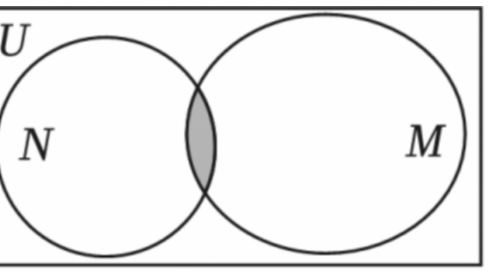
\includegraphics[width=0.30\textwidth]{figures/gao87_q14_venn.png}
\end{center}

\keepwithprev
A. $3$ 个\qquad B. $2$ 个\qquad C. $1$ 个\qquad D. 无穷多个

\ifanswer
\solbegin
\step{阴影部分所示的集合为 $M\cap N$，}
\step{$M=\{x\mid-1\leqslant x\leqslant3\}$，在此范围内的奇数有 $1$ 和 $3$，}
\step{所以集合 $M\cap N=\{1,3\}$ 共有 $2$ 个元素，故选 $B$.}
\solend
\fi

\item 已知实数 $a,b,c$ 满足 $a>b$，则下列不等式成立的是\mbox{（\quad）}

\keepwithprev
A. $-\dfrac1a<\dfrac1b$\qquad B. $a^2>b^2$\qquad C. $a\lvert c\rvert>b\lvert c\rvert$\qquad D. $\dfrac a{c^2+1}>\dfrac b{c^2+1}$

\ifanswer
\solbegin
\step{若 $a=1,b=-1$，则 $-1=-\dfrac1a=\dfrac1b=1$，$a^2=b^2=1$，则 AB 错误；}
\step{若 $a>b,c=0$，则 $a\lvert c\rvert=b\lvert c\rvert=0$，则 C 错误；}
\step{因为 $c^2+1\geqslant1$，所以 $0<\dfrac1{c^2+1}\leqslant1$，又 $a>b$，所以 $\dfrac a{c^2+1}>\dfrac b{c^2+1}$，}
\step{则 D 正确.}
\step{故选 $D$.}
\solend
\fi

\item 设集合 $P_1=\{x\mid x^2+ax+1>0\}$，$P_2=\{x\mid x^2+ax+2>0\}$，$Q_1=\{x\mid x^2+x+b>0\}$，
$Q_2=\{x\mid x^2+2x+b>0\}$，其中 $a$、$b\in\R$，下列说法中正确的是\mbox{（\quad）}

\keepwithprev
A. 对任意 $a$，$P_1$ 是 $P_2$ 的子集，对任意 $b$，$Q_1$ 不是 $Q_2$ 的子集

B. 对任意 $a$，$P_1$ 是 $P_2$ 的子集，存在 $b$，使得 $Q_1$ 是 $Q_2$ 的子集

C. 存在 $a$，使得 $P_1$ 不是 $P_2$ 的子集，对任意 $b$，$Q_1$ 不是 $Q_2$ 的子集

D. 存在 $a$，使得 $P_1$ 不是 $P_2$ 的子集，存在 $b$，使得 $Q_1$ 是 $Q_2$ 的子集

\ifanswer
\solbegin
\step{对于集合 $P_1=\{x\mid x^2+ax+1>0\}$，$P_2=\{x\mid x^2+ax+2>0\}$，}
\step{得当 $m\in P_1$ 时，即 $m^2+am+1>0$，得 $m^2+am+2>0$，}
\step{即有 $m\in P_2$，得对任意 $a$，$P_1$ 是 $P_2$ 的子集，}
\step{对于集合 $Q_1=\{x\mid x^2+x+b>0\}$，$Q_2=\{x\mid x^2+2x+b>0\}$，}
\step{当 $b=6$ 时，$Q_1=\{x\mid x^2+x+6>0\}=\R$，$Q_2=\{x\mid x^2+2x+6>0\}=\R$，}
\step{得 $Q_1$ 是 $Q_2$ 的子集，}
\step{当 $b=1$ 时，$Q_1=\{x\mid x^2+x+1>0\}=\R$，}
\step{$Q_2=\{x\mid x^2+2x+1>0\}=\{x\mid x\neq-1\}$，得 $Q_1$ 不是 $Q_2$ 的子集，}
\step{所以存在 $b$，使得 $Q_1$ 是 $Q_2$ 的子集，故选 $B$.}
\solend
\fi

\end{enumerate}

\bigsec{三、解答题}

\begin{enumerate}
\setcounter{enumi}{16}

\item 设 $m$ 为实数，求关于 $x$ 与 $y$ 的二元一次方程组 $\begin{cases}y=x+m\\ mx-y=4\end{cases}$ 的解集.

\ansspace*[8]

\ifanswer
\solbegin
\step{消去 $y$ 得 $(m-1)x=m+4$，}
\step{当 $m-1=0$，即 $m=1$ 时，$0=5$ 不成立，则 $x$ 无解，原方程组的解集为 $\varnothing$；}
\step{当 $m-1\neq0$，即 $m\neq1$ 时，则 $x=\dfrac{m+4}{m-1}$，$y=\dfrac{m+4}{m-1}+m=\dfrac{m^2+4}{m-1}$，}
\step{原方程组的解集为 $\left\{\left(\dfrac{m+4}{m-1},\dfrac{m^2+4}{m-1}\right)\right\}$.}
\step{综上所述，当 $m=1$ 时，方程组的解集为 $\varnothing$；}
\step{当 $m\neq1$ 时，方程组的解集为 $\left\{\left(\dfrac{m+4}{m-1},\dfrac{m^2+4}{m-1}\right)\right\}$.}
\solend
\fi

\item 设 $x<y<0$，试比较 $(x^2+y^2)(x-y)$ 与 $(x^2-y^2)(x+y)$ 的大小.

\ansspace*[9]

\ifanswer
\solbegin
\step{$(x^2+y^2)(x-y)-(x^2-y^2)(x+y)=(x-y)[x^2+y^2-(x+y)^2]=-2xy(x-y)$，}
\step{因为 $x<y<0$，所以 $xy>0$，$x-y<0$，所以 $-2xy(x-y)>0$，}
\step{即 $(x^2+y^2)(x-y)>(x^2-y^2)(x+y)$.}
\solend
\fi

\item 已知全集 $U=\R$，集合 $A=\left\{x\left|\dfrac{2+x}{3-x}>0\right.\right\}$，集合 $B=\{x\mid\lvert x-2\rvert>3\}$.

（1）求 $A\cup B$、$\overline A\cap B$.

（2）若集合 $C=\{x\mid x\leqslant a\}$，且 $A\cap C=A$，求实数 $a$ 的范围.

\ansspace*[10]

\ifanswer
\solbegin
\stepm{（1）}{由 $\lvert x-2\rvert>3$ 得 $x-2>3$ 或 $x-2<-3$，即 $x<-1$ 或 $x>5$，}
\step{所以 $B=(-\infty,-1)\cup(5,+\infty)$，}
\step{$A=\left\{x\left|\dfrac{2+x}{3-x}>0\right.\right\}=\{x\mid(2+x)(3-x)>0\}=(-2,3)$，}
\step{所以 $A\cup b=(-\infty,3)\cup(5m+\infty)$，}
\step{$\overline A=(-\infty,-2]\cup[3,+\infty)$，$\overline A\cap B=(-\infty,-2]\cup(5,+\infty)$.}
\stepm{（2）}{因为 $A\cap C=A$，所以 $A\subseteq C$，}
\step{因为 $A=(-2,3)$，所以实数 $a$ 的取值范围为 $\{a\mid a\geqslant3\}$.}
\solend
\fi

\item 已知函数 $f(x)=ax^2+4x+b\,(a<0,a,b\in\R)$，设关于 $x$ 的方程 $f(x)=0$ 的两实根为 $x_1$、
$x_2$，方程 $f(x)=x$ 的两实根为 $\alpha,\beta$.

（1）不等式 $f(x)<0$ 的解集是 $(-\infty,-3)\cup(5,+\infty)$，求不等式 $bx^2-ax-4<0$ 的解集；

（2）若 $a,b$ 均为负整数，且 $\lvert\alpha-\beta\rvert=1$，求 $f(x)$ 的解析式.

\ansspace*[12]

\ifanswer
\solbegin
\stepm{（1）}{$ax^2+4x+b<0$ 的解集为 $(-\infty,-3)\cup(5,+\infty)$，}
\step{所以 $-3,5$ 是方程 $ax^2+4x+b=0$ 的两根，所以 $\begin{cases}-3+5=-\dfrac4a\\ -3\times5=\dfrac ba\end{cases}\Rightarrow\begin{cases}a=-2\\ b=30\end{cases}$，}
\step{所以 $bx^2-ax-4<0$ 为 $30x^2+2x-4<0\Rightarrow15x^2+x-2<0$，}
\step{所以 $(3x-1)(5x+2)<0\Rightarrow-\dfrac25<x<\dfrac13$，}
\step{所以所求不等式的解集为 $\left\{x\left|-\dfrac25<x<\dfrac13\right.\right\}$.}
\stepm{（2）}{由题意得 $f(x)=ax^2+4x+b\,(a<0,a,b\in\R)$ 有两个不等实根为 $\alpha$、$\beta$，}
\step{所以 $\Delta=9-4ab>0$，$\alpha+\beta=-\dfrac3a$，$\alpha\beta=\dfrac ba$.}
\step{由 $\lvert\alpha-\beta\rvert=1$ 得 $(\alpha-\beta)^2=1$，即 $(\alpha+\beta)^2-4\alpha\beta=\dfrac9{a^2}-\dfrac{4b}a=1$，}
\step{所以 $9-4ab=a^2$，即 $a^2+4ab=9\,(a<0,a,b\in\R)$.}
\step{因为 $a,b$ 均为负整数，}
\step{所以 $\begin{cases}a=-1\\ a+4b=-9\end{cases}$ 或 $\begin{cases}a=-9\\ a+4b=-1\end{cases}$ 或 $\begin{cases}a=-3\\ a+4b=-3\end{cases}$，}
\step{显然后两种情况不合题意，应舍去，从而有 $\begin{cases}a=-1\\ a+4b=-9\end{cases}$，解得 $a=-1$，$b=-2$.}
\step{故所求函数解析式为 $f(x)=-x^2+4x-2$.}
\solend
\fi

\item 已知集合 $A=\{x\mid x=m^2+n^2,m\in\Z,n\in\Z\}$.

（1）判断 $2,5,25$ 是否属于集合 $A$；

（2）若正整数 $y$ 能表示为某个整数的平方，$z\in A$，证明：$yz\in A$；

（3）若集合 $B=\{x\mid x=4k+3,k\in\Z\}$，证明：$A\cap B=\varnothing$.

\ansspace*[14]

\ifanswer
\solbegin
\stepm{（1）}{由 $2=1^2+1^2$，$5=1^2+2^2$，$25=3^2+4^2$ 得 $2,5,25$ 属于集合 $A$；}
\stepm{（2）}{设 $y=a^2\,(a\in\Z)$，由 $z\in A$，设 $z=b^2+c^2\,(b\in\Z,c\in\Z)$，}
\step{则 $yz=a^2(b^2+c^2)=(ab)^2+(ac)^2$，}
\step{因为 $a\in\Z$，$b\in\Z$，$c\in\Z$，所以 $ab\in\Z$，$ac\in\Z$，所以 $yz\in A$；}
\stepm{（3）}{①当 $m$、$n$ 都为偶数时，设 $m=2k_1\,(k_1\in\Z)$，$n=2k_2\,(k_2\in\Z)$，}
\step{则 $x=m^2+n^2=4k_1^2+4k_2^2=4(k_1^2+k_2^2)$，此时 $x$ 为 $4$ 的倍数，}
\step{因为偶数 $\notin B$，所以 $A\cap B=\varnothing$；}
\step{②当 $m$、$n$ 都为奇数时，设 $m=2k_1+1\,(k_1\in\Z)$，$n=2k_2+1\,(k_2\in\Z)$，}
\step{则 $x=m^2+n^2=(2k_1+1)^2+(2k_2+1)^2=4(k_1^2+k_2^2+k_1+k_2)+2$，}
\step{此时 $x$ 为 $2$ 的倍数，因为偶数 $\notin B$，所以 $A\cap B=\varnothing$；}
\step{③当 $m$、$n$ 一奇一偶时，设 $m=2k_1+1\,(k_1\in\Z)$，$n=2k_2\,(k_2\in\Z)$，}
\step{则 $x=m^2+n^2=(2k_1+1)^2+(2k_2)^2=4(k_1^2+k_2^2+k_1)+1$，}
\step{此时 $x$ 被 $4$ 除余 $1$，而 $B$ 中元素被 $4$ 除余 $3$，此时 $A\cap B=\varnothing$.}
\step{综上，$A\cap B=\varnothing$.}
\solend
\fi

\end{enumerate}

\end{document}
"
% 紧凑版：xelatex "\def\iscompact{1}% 高一87_五十四中学_10月月考.tex
%   —— 高一上数学“2026-2027 年五十四中学高一上 10 月月考”（讲评版）
% 试卷版：xelatex 高一87_五十四中学_10月月考.tex
% 答案版：xelatex "\def\isanswer{1}\input{高一87_五十四中学_10月月考.tex}"
% 紧凑版：xelatex "\def\iscompact{1}\input{高一87_五十四中学_10月月考.tex}"
%
% 原始材料：微信公众号“魔都数学加油站”文章，连载“27学年高一87”；
% 原文标题“27学年高一87——2026-2027年上海市五十四中学高一上10月月考”；
% 原文链接：https://mp.weixin.qq.com/s/pqPpSGQt0AhydcpaB8uEkQ。
% 页面标注发布时间 2026-10-27 17:43（上海）。
% 正文为 7 张 PNG 页（`原图/高一87_五十四中学_10月月考/01..07.png`），
% 尺寸混排（第 1、2 页为 4762×6735，第 3—7 页为 2560×3620），均按页序读取。
%
% 篇幅与题号：原卷自第 3 题起编号（第 1、2 题不在原文内）。填空题 3—12（10 题）、
% 选择题 13—16（4 题）、解答题 17—21（5 题），共 19 题。
%
% 讲评版：第 3、5、6 题只印【答案】（“$x\leqslant1$ 且 $y\leqslant1$”“$\{(2,6),(6,2)\}$”
% “$(-1,3]$”），本稿只给 \ans{}；其余 16 题印【解析】，其中选择题答案在解析末句
% “故选 A／B／D／B”。第 14 题题干带一幅韦恩图（裁自第 3 页原图、去粉色水印后转灰度），
% 三版都出。
%
% 副标题：原卷未印副标题。本稿按内容标作“集合与常用逻辑用语、不等式”。
%
% 原卷笔误/存疑（均照录未改，正文对应处另有 % 注）：
%   ① 第 19 题 (1) 解析作“所以 $A\cup b=(-\infty,3)\cup(5m+\infty)$”，两处均系排印错：
%      按上下文应为“$A\cup B=(-\infty,3)\cup(5,+\infty)$”（同页下一行 $\overline A\cap B$
%      的端点 $5$、$+\infty$ 也印证这一点）。原卷印作 $b$ 与 $5m+\infty$，照录未改。
%
% 与原卷的排版差异：
%   ① 原卷每题下直接印【答案】/【解析】，本稿按全稿惯例将答案与解析置于答案版；
%   ② 原卷未印副标题，本稿补出；填空横线统一排 \blankline[4.4em]；
%   ③ 原卷数集记号排斜体 $R$、$Z$、$N$，本稿按全稿惯例改用 $\R$、$\Z$、$\N$；
%   ④ 第 17—21 题的子问用行内“（1）（2）（3）”段，解析中的子问标号用 \stepm；
%   ⑤ 解答题按惯例加 \ansspace；选择题括号排 \mbox{（\quad）}。
%
% 行数核对：逐题数 \step/\stepm 条数，合计 86 条（Q4：1；Q7：4；Q8：2；Q9：2；Q10：3；
% Q11：9；Q12：3；Q13：2；Q14：3；Q15：5；Q16：9；Q17：6；Q18：3；Q19：7；Q20：13；
% Q21：14）；第 3、5、6 题只印【答案】，提 \ans{}，不计入 \step 账。原卷解析的换行
% 按语意合并，未逐行强拆。
%
\documentclass[a4paper,11pt]{article}
\usepackage{common}

\begin{document}

\examtitlest[7]{2026--2027 年五十四中学高一上 10 月月考}{集合与常用逻辑用语、不等式}

\bigsec{一、填空题}

\begin{enumerate}
\setcounter{enumi}{2}

\item “$x>1$ 或 $y>1$”的否定形式为\blankline[4.4em].

\ifanswer
\ans{$x\leqslant1$ 且 $y\leqslant1$}
\fi

\item 已知 $1<a<2$，$-3<b<3$，则 $a+b$ 的取值范围是\blankline[4.4em].

\ifanswer
\solbegin
\step{由不等式的可加性得 $-2<a+b<5$，故 $a+b$ 的取值范围是 $(-2,5)$.}
\solend
\fi

\item 方程组 $\begin{cases}x+y=8\\ xy=12\end{cases}$ 的解集为\blankline[4.4em].

\ifanswer
\ans{$\{(2,6),(6,2)\}$}
\fi

\item 不等式 $\dfrac{x-3}{x+1}\leqslant0$ 解集为\blankline[4.4em].

\ifanswer
\ans{$(-1,3]$}
\fi

\item 已知集合 $A=\{x\mid y=\sqrt{x+1}\}$，$B=\{y\mid y=x^2+5\}$，则 $A\cup B=\blankline[4.4em]$.

\ifanswer
\solbegin
\step{对于函数 $y=\sqrt{x+1}$，则 $x+1\geqslant0$，解得 $x\geqslant-1$，}
\step{所以 $A=\{x\mid y=\sqrt{x+1}\}=\{x\mid x\geqslant-1\}$，}
\step{因为 $x^2\geqslant0$，所以 $y=x^2+5\geqslant5$，所以 $B=\{y\mid y=x^2+5\}=\{y\mid y\geqslant5\}$，}
\step{所以 $A\cup B=\{x\mid x\geqslant-1\}$.}
\solend
\fi

\item 已知关于 $x$ 的不等式 $\lvert x+a\rvert<b$ 的解集为 $\{x\mid2<x<4\}$，则 $a+b$ 的值是\blankline[4.4em].

\ifanswer
\solbegin
\step{由 $\lvert x+a\rvert<b$，得 $-b-a<x<b-a$，则 $\begin{cases}-b-a=2\\ b-a=4\end{cases}$，解得 $a=-3$，$b=1$，}
\step{所以 $a+b=-2$.}
\solend
\fi

\item 已知一元二次方程 $x^2-2mx+m-1=0$ 的两实根为 $x_1,x_2$，且 $x_1^2+x_2^2=4$，则实数 $m$ 的值
是\blankline[4.4em].

\ifanswer
\solbegin
\step{由题意得 $x_1+x_2=2m$，$x_1x_2=m-1$，}
\step{所以 $x_1^2+x_2^2=(x_1+x_2)^2-2x_1x_2=4m^2-2m+2=4$，解得 $m=1$ 或 $m=-\dfrac12$.}
\solend
\fi

\item 已知集合 $A=\{x\mid x^2-x-6=0\}$，$B=\{y\mid ay-1=0\}$，若 $A\cap B=B$，则实数
$a=\blankline[4.4em]$.

\ifanswer
\solbegin
\step{$A=\{-2,3\}$，由 $A\cap B=B$，得 $B\subseteq A$，而 $B=\{y\mid ay-1=0\}$，}
\step{则当 $B=\varnothing$ 时，$a=0$；当 $B=\{-2\}$ 时，$-2a-1=0$，解得 $a=-\dfrac12$；}
\step{当 $B=\{3\}$ 时，$3a-1=0$，解得 $a=\dfrac13$，所以实数 $a$ 的值为 $-\dfrac12$ 或 $0$ 或 $\dfrac13$.}
\solend
\fi

\item 已知集合 $A=\{x\mid(m-1)x^2+(m-1)x+2\leqslant0,x\in\R\}$，$B=\left\{x\left|\dfrac{2x-1}{x^2+x+1}>1,x\in\R\right.\right\}$，
且 $A\cap B=A$，则实数 $m$ 的取值范围是\blankline[4.4em].

\ifanswer
\solbegin
\step{因为 $\dfrac{2x-1}{x^2+x+1}>1$，所以 $x^2-x+2<0$，显然不等式无解，}
\step{所以 $B=\left\{x\left|\dfrac{2x-1}{x^2+x+1}>1,x\in\R\right.\right\}=\varnothing$，而 $A\cap B=A$，则 $A=\varnothing$，}
\step{①当 $m=1$ 时，$2\leqslant0$ 不成立，此时 $A=\varnothing$，}
\step{②当 $m<1$ 时，$m-1<0$，函数 $y=(m-1)x^2+(m-1)x+2$，开口向下，}
\step{不等式 $(m-1)x^2+(m-1)x+2\leqslant0$ 有解，$A\neq\varnothing$，}
\step{③当 $m>1$ 时，函数 $y=(m-1)x^2+(m-1)x+2$，开口向上，}
\step{若不等式 $(m-1)x^2+(m-1)x+2\leqslant0$ 无解，}
\step{只需 $\Delta=(m-1)^2-8(m-1)<0$，解得 $1<m<9$，}
\step{综上，$m$ 的取值范围是 $[1,9]$.}
\solend
\fi

\item 设 $A$ 是整数集的一个非空子集，对于 $k\in A$，如果 $k-1\notin A$ 且 $k+1\notin A$，那么 $k$ 是 $A$
的一个“孤立元”. 给定 $S=\{1,2,3,4,5,6,7,8\}$，由 $S$ 的 $3$ 个元素构成的所有集合中，不含
“孤立元”的集合共有\blankline[3.6em]个.

\ifanswer
\solbegin
\step{由题意得，“孤立元”即为在集合中无与之相邻的元素，}
\step{满足条件的集合有 $\{1,2,3\},\{2,3,4\},\{3,4,5\},\{4,5,6\},\{5,6,7\},\{6,7,8\}$，}
\step{共 $6$ 个集合.}
\solend
\fi

\end{enumerate}

\bigsec{二、选择题}

\begin{enumerate}
\setcounter{enumi}{12}

\item “$m=2$”是“$m^2=4$”的\mbox{（\quad）}条件.

\keepwithprev
A. 充分非必要条件\qquad B. 必要非充分条件

C. 充要条件\qquad D. 既非充分又非必要条件

\ifanswer
\solbegin
\step{由 $m^2=4$，解得 $m=\pm2$，故“$m=2$”是“$m^2=4$”的充分不必要条件，}
\step{故选 $A$.}
\solend
\fi

\item 已知全集 $U=\R$，集合 $M=\{x\mid\lvert x-1\rvert\leqslant2\}$ 和 $N=\{x\mid x=2k-1,k\in\Z\}$ 的关系
的韦恩（$Venn$）图如图所示，则阴影部分所示的集合的元素共有\mbox{（\quad）}

\begin{center}
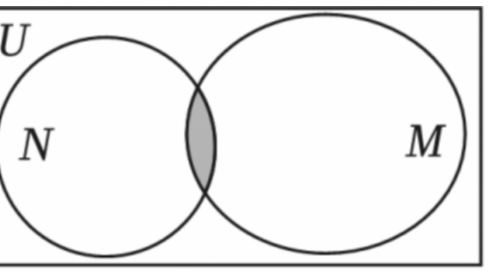
\includegraphics[width=0.30\textwidth]{figures/gao87_q14_venn.png}
\end{center}

\keepwithprev
A. $3$ 个\qquad B. $2$ 个\qquad C. $1$ 个\qquad D. 无穷多个

\ifanswer
\solbegin
\step{阴影部分所示的集合为 $M\cap N$，}
\step{$M=\{x\mid-1\leqslant x\leqslant3\}$，在此范围内的奇数有 $1$ 和 $3$，}
\step{所以集合 $M\cap N=\{1,3\}$ 共有 $2$ 个元素，故选 $B$.}
\solend
\fi

\item 已知实数 $a,b,c$ 满足 $a>b$，则下列不等式成立的是\mbox{（\quad）}

\keepwithprev
A. $-\dfrac1a<\dfrac1b$\qquad B. $a^2>b^2$\qquad C. $a\lvert c\rvert>b\lvert c\rvert$\qquad D. $\dfrac a{c^2+1}>\dfrac b{c^2+1}$

\ifanswer
\solbegin
\step{若 $a=1,b=-1$，则 $-1=-\dfrac1a=\dfrac1b=1$，$a^2=b^2=1$，则 AB 错误；}
\step{若 $a>b,c=0$，则 $a\lvert c\rvert=b\lvert c\rvert=0$，则 C 错误；}
\step{因为 $c^2+1\geqslant1$，所以 $0<\dfrac1{c^2+1}\leqslant1$，又 $a>b$，所以 $\dfrac a{c^2+1}>\dfrac b{c^2+1}$，}
\step{则 D 正确.}
\step{故选 $D$.}
\solend
\fi

\item 设集合 $P_1=\{x\mid x^2+ax+1>0\}$，$P_2=\{x\mid x^2+ax+2>0\}$，$Q_1=\{x\mid x^2+x+b>0\}$，
$Q_2=\{x\mid x^2+2x+b>0\}$，其中 $a$、$b\in\R$，下列说法中正确的是\mbox{（\quad）}

\keepwithprev
A. 对任意 $a$，$P_1$ 是 $P_2$ 的子集，对任意 $b$，$Q_1$ 不是 $Q_2$ 的子集

B. 对任意 $a$，$P_1$ 是 $P_2$ 的子集，存在 $b$，使得 $Q_1$ 是 $Q_2$ 的子集

C. 存在 $a$，使得 $P_1$ 不是 $P_2$ 的子集，对任意 $b$，$Q_1$ 不是 $Q_2$ 的子集

D. 存在 $a$，使得 $P_1$ 不是 $P_2$ 的子集，存在 $b$，使得 $Q_1$ 是 $Q_2$ 的子集

\ifanswer
\solbegin
\step{对于集合 $P_1=\{x\mid x^2+ax+1>0\}$，$P_2=\{x\mid x^2+ax+2>0\}$，}
\step{得当 $m\in P_1$ 时，即 $m^2+am+1>0$，得 $m^2+am+2>0$，}
\step{即有 $m\in P_2$，得对任意 $a$，$P_1$ 是 $P_2$ 的子集，}
\step{对于集合 $Q_1=\{x\mid x^2+x+b>0\}$，$Q_2=\{x\mid x^2+2x+b>0\}$，}
\step{当 $b=6$ 时，$Q_1=\{x\mid x^2+x+6>0\}=\R$，$Q_2=\{x\mid x^2+2x+6>0\}=\R$，}
\step{得 $Q_1$ 是 $Q_2$ 的子集，}
\step{当 $b=1$ 时，$Q_1=\{x\mid x^2+x+1>0\}=\R$，}
\step{$Q_2=\{x\mid x^2+2x+1>0\}=\{x\mid x\neq-1\}$，得 $Q_1$ 不是 $Q_2$ 的子集，}
\step{所以存在 $b$，使得 $Q_1$ 是 $Q_2$ 的子集，故选 $B$.}
\solend
\fi

\end{enumerate}

\bigsec{三、解答题}

\begin{enumerate}
\setcounter{enumi}{16}

\item 设 $m$ 为实数，求关于 $x$ 与 $y$ 的二元一次方程组 $\begin{cases}y=x+m\\ mx-y=4\end{cases}$ 的解集.

\ansspace*[8]

\ifanswer
\solbegin
\step{消去 $y$ 得 $(m-1)x=m+4$，}
\step{当 $m-1=0$，即 $m=1$ 时，$0=5$ 不成立，则 $x$ 无解，原方程组的解集为 $\varnothing$；}
\step{当 $m-1\neq0$，即 $m\neq1$ 时，则 $x=\dfrac{m+4}{m-1}$，$y=\dfrac{m+4}{m-1}+m=\dfrac{m^2+4}{m-1}$，}
\step{原方程组的解集为 $\left\{\left(\dfrac{m+4}{m-1},\dfrac{m^2+4}{m-1}\right)\right\}$.}
\step{综上所述，当 $m=1$ 时，方程组的解集为 $\varnothing$；}
\step{当 $m\neq1$ 时，方程组的解集为 $\left\{\left(\dfrac{m+4}{m-1},\dfrac{m^2+4}{m-1}\right)\right\}$.}
\solend
\fi

\item 设 $x<y<0$，试比较 $(x^2+y^2)(x-y)$ 与 $(x^2-y^2)(x+y)$ 的大小.

\ansspace*[9]

\ifanswer
\solbegin
\step{$(x^2+y^2)(x-y)-(x^2-y^2)(x+y)=(x-y)[x^2+y^2-(x+y)^2]=-2xy(x-y)$，}
\step{因为 $x<y<0$，所以 $xy>0$，$x-y<0$，所以 $-2xy(x-y)>0$，}
\step{即 $(x^2+y^2)(x-y)>(x^2-y^2)(x+y)$.}
\solend
\fi

\item 已知全集 $U=\R$，集合 $A=\left\{x\left|\dfrac{2+x}{3-x}>0\right.\right\}$，集合 $B=\{x\mid\lvert x-2\rvert>3\}$.

（1）求 $A\cup B$、$\overline A\cap B$.

（2）若集合 $C=\{x\mid x\leqslant a\}$，且 $A\cap C=A$，求实数 $a$ 的范围.

\ansspace*[10]

\ifanswer
\solbegin
\stepm{（1）}{由 $\lvert x-2\rvert>3$ 得 $x-2>3$ 或 $x-2<-3$，即 $x<-1$ 或 $x>5$，}
\step{所以 $B=(-\infty,-1)\cup(5,+\infty)$，}
\step{$A=\left\{x\left|\dfrac{2+x}{3-x}>0\right.\right\}=\{x\mid(2+x)(3-x)>0\}=(-2,3)$，}
\step{所以 $A\cup b=(-\infty,3)\cup(5m+\infty)$，}
\step{$\overline A=(-\infty,-2]\cup[3,+\infty)$，$\overline A\cap B=(-\infty,-2]\cup(5,+\infty)$.}
\stepm{（2）}{因为 $A\cap C=A$，所以 $A\subseteq C$，}
\step{因为 $A=(-2,3)$，所以实数 $a$ 的取值范围为 $\{a\mid a\geqslant3\}$.}
\solend
\fi

\item 已知函数 $f(x)=ax^2+4x+b\,(a<0,a,b\in\R)$，设关于 $x$ 的方程 $f(x)=0$ 的两实根为 $x_1$、
$x_2$，方程 $f(x)=x$ 的两实根为 $\alpha,\beta$.

（1）不等式 $f(x)<0$ 的解集是 $(-\infty,-3)\cup(5,+\infty)$，求不等式 $bx^2-ax-4<0$ 的解集；

（2）若 $a,b$ 均为负整数，且 $\lvert\alpha-\beta\rvert=1$，求 $f(x)$ 的解析式.

\ansspace*[12]

\ifanswer
\solbegin
\stepm{（1）}{$ax^2+4x+b<0$ 的解集为 $(-\infty,-3)\cup(5,+\infty)$，}
\step{所以 $-3,5$ 是方程 $ax^2+4x+b=0$ 的两根，所以 $\begin{cases}-3+5=-\dfrac4a\\ -3\times5=\dfrac ba\end{cases}\Rightarrow\begin{cases}a=-2\\ b=30\end{cases}$，}
\step{所以 $bx^2-ax-4<0$ 为 $30x^2+2x-4<0\Rightarrow15x^2+x-2<0$，}
\step{所以 $(3x-1)(5x+2)<0\Rightarrow-\dfrac25<x<\dfrac13$，}
\step{所以所求不等式的解集为 $\left\{x\left|-\dfrac25<x<\dfrac13\right.\right\}$.}
\stepm{（2）}{由题意得 $f(x)=ax^2+4x+b\,(a<0,a,b\in\R)$ 有两个不等实根为 $\alpha$、$\beta$，}
\step{所以 $\Delta=9-4ab>0$，$\alpha+\beta=-\dfrac3a$，$\alpha\beta=\dfrac ba$.}
\step{由 $\lvert\alpha-\beta\rvert=1$ 得 $(\alpha-\beta)^2=1$，即 $(\alpha+\beta)^2-4\alpha\beta=\dfrac9{a^2}-\dfrac{4b}a=1$，}
\step{所以 $9-4ab=a^2$，即 $a^2+4ab=9\,(a<0,a,b\in\R)$.}
\step{因为 $a,b$ 均为负整数，}
\step{所以 $\begin{cases}a=-1\\ a+4b=-9\end{cases}$ 或 $\begin{cases}a=-9\\ a+4b=-1\end{cases}$ 或 $\begin{cases}a=-3\\ a+4b=-3\end{cases}$，}
\step{显然后两种情况不合题意，应舍去，从而有 $\begin{cases}a=-1\\ a+4b=-9\end{cases}$，解得 $a=-1$，$b=-2$.}
\step{故所求函数解析式为 $f(x)=-x^2+4x-2$.}
\solend
\fi

\item 已知集合 $A=\{x\mid x=m^2+n^2,m\in\Z,n\in\Z\}$.

（1）判断 $2,5,25$ 是否属于集合 $A$；

（2）若正整数 $y$ 能表示为某个整数的平方，$z\in A$，证明：$yz\in A$；

（3）若集合 $B=\{x\mid x=4k+3,k\in\Z\}$，证明：$A\cap B=\varnothing$.

\ansspace*[14]

\ifanswer
\solbegin
\stepm{（1）}{由 $2=1^2+1^2$，$5=1^2+2^2$，$25=3^2+4^2$ 得 $2,5,25$ 属于集合 $A$；}
\stepm{（2）}{设 $y=a^2\,(a\in\Z)$，由 $z\in A$，设 $z=b^2+c^2\,(b\in\Z,c\in\Z)$，}
\step{则 $yz=a^2(b^2+c^2)=(ab)^2+(ac)^2$，}
\step{因为 $a\in\Z$，$b\in\Z$，$c\in\Z$，所以 $ab\in\Z$，$ac\in\Z$，所以 $yz\in A$；}
\stepm{（3）}{①当 $m$、$n$ 都为偶数时，设 $m=2k_1\,(k_1\in\Z)$，$n=2k_2\,(k_2\in\Z)$，}
\step{则 $x=m^2+n^2=4k_1^2+4k_2^2=4(k_1^2+k_2^2)$，此时 $x$ 为 $4$ 的倍数，}
\step{因为偶数 $\notin B$，所以 $A\cap B=\varnothing$；}
\step{②当 $m$、$n$ 都为奇数时，设 $m=2k_1+1\,(k_1\in\Z)$，$n=2k_2+1\,(k_2\in\Z)$，}
\step{则 $x=m^2+n^2=(2k_1+1)^2+(2k_2+1)^2=4(k_1^2+k_2^2+k_1+k_2)+2$，}
\step{此时 $x$ 为 $2$ 的倍数，因为偶数 $\notin B$，所以 $A\cap B=\varnothing$；}
\step{③当 $m$、$n$ 一奇一偶时，设 $m=2k_1+1\,(k_1\in\Z)$，$n=2k_2\,(k_2\in\Z)$，}
\step{则 $x=m^2+n^2=(2k_1+1)^2+(2k_2)^2=4(k_1^2+k_2^2+k_1)+1$，}
\step{此时 $x$ 被 $4$ 除余 $1$，而 $B$ 中元素被 $4$ 除余 $3$，此时 $A\cap B=\varnothing$.}
\step{综上，$A\cap B=\varnothing$.}
\solend
\fi

\end{enumerate}

\end{document}
"
%
% 原始材料：微信公众号“魔都数学加油站”文章，连载“27学年高一87”；
% 原文标题“27学年高一87——2026-2027年上海市五十四中学高一上10月月考”；
% 原文链接：https://mp.weixin.qq.com/s/pqPpSGQt0AhydcpaB8uEkQ。
% 页面标注发布时间 2026-10-27 17:43（上海）。
% 正文为 7 张 PNG 页（`原图/高一87_五十四中学_10月月考/01..07.png`），
% 尺寸混排（第 1、2 页为 4762×6735，第 3—7 页为 2560×3620），均按页序读取。
%
% 篇幅与题号：原卷自第 3 题起编号（第 1、2 题不在原文内）。填空题 3—12（10 题）、
% 选择题 13—16（4 题）、解答题 17—21（5 题），共 19 题。
%
% 讲评版：第 3、5、6 题只印【答案】（“$x\leqslant1$ 且 $y\leqslant1$”“$\{(2,6),(6,2)\}$”
% “$(-1,3]$”），本稿只给 \ans{}；其余 16 题印【解析】，其中选择题答案在解析末句
% “故选 A／B／D／B”。第 14 题题干带一幅韦恩图（裁自第 3 页原图、去粉色水印后转灰度），
% 三版都出。
%
% 副标题：原卷未印副标题。本稿按内容标作“集合与常用逻辑用语、不等式”。
%
% 原卷笔误/存疑（均照录未改，正文对应处另有 % 注）：
%   ① 第 19 题 (1) 解析作“所以 $A\cup b=(-\infty,3)\cup(5m+\infty)$”，两处均系排印错：
%      按上下文应为“$A\cup B=(-\infty,3)\cup(5,+\infty)$”（同页下一行 $\overline A\cap B$
%      的端点 $5$、$+\infty$ 也印证这一点）。原卷印作 $b$ 与 $5m+\infty$，照录未改。
%
% 与原卷的排版差异：
%   ① 原卷每题下直接印【答案】/【解析】，本稿按全稿惯例将答案与解析置于答案版；
%   ② 原卷未印副标题，本稿补出；填空横线统一排 \blankline[4.4em]；
%   ③ 原卷数集记号排斜体 $R$、$Z$、$N$，本稿按全稿惯例改用 $\R$、$\Z$、$\N$；
%   ④ 第 17—21 题的子问用行内“（1）（2）（3）”段，解析中的子问标号用 \stepm；
%   ⑤ 解答题按惯例加 \ansspace；选择题括号排 \mbox{（\quad）}。
%
% 行数核对：逐题数 \step/\stepm 条数，合计 86 条（Q4：1；Q7：4；Q8：2；Q9：2；Q10：3；
% Q11：9；Q12：3；Q13：2；Q14：3；Q15：5；Q16：9；Q17：6；Q18：3；Q19：7；Q20：13；
% Q21：14）；第 3、5、6 题只印【答案】，提 \ans{}，不计入 \step 账。原卷解析的换行
% 按语意合并，未逐行强拆。
%
\documentclass[a4paper,11pt]{article}
\usepackage{common}

\begin{document}

\examtitlest[7]{2026--2027 年五十四中学高一上 10 月月考}{集合与常用逻辑用语、不等式}

\bigsec{一、填空题}

\begin{enumerate}
\setcounter{enumi}{2}

\item “$x>1$ 或 $y>1$”的否定形式为\blankline[4.4em].

\ifanswer
\ans{$x\leqslant1$ 且 $y\leqslant1$}
\fi

\item 已知 $1<a<2$，$-3<b<3$，则 $a+b$ 的取值范围是\blankline[4.4em].

\ifanswer
\solbegin
\step{由不等式的可加性得 $-2<a+b<5$，故 $a+b$ 的取值范围是 $(-2,5)$.}
\solend
\fi

\item 方程组 $\begin{cases}x+y=8\\ xy=12\end{cases}$ 的解集为\blankline[4.4em].

\ifanswer
\ans{$\{(2,6),(6,2)\}$}
\fi

\item 不等式 $\dfrac{x-3}{x+1}\leqslant0$ 解集为\blankline[4.4em].

\ifanswer
\ans{$(-1,3]$}
\fi

\item 已知集合 $A=\{x\mid y=\sqrt{x+1}\}$，$B=\{y\mid y=x^2+5\}$，则 $A\cup B=\blankline[4.4em]$.

\ifanswer
\solbegin
\step{对于函数 $y=\sqrt{x+1}$，则 $x+1\geqslant0$，解得 $x\geqslant-1$，}
\step{所以 $A=\{x\mid y=\sqrt{x+1}\}=\{x\mid x\geqslant-1\}$，}
\step{因为 $x^2\geqslant0$，所以 $y=x^2+5\geqslant5$，所以 $B=\{y\mid y=x^2+5\}=\{y\mid y\geqslant5\}$，}
\step{所以 $A\cup B=\{x\mid x\geqslant-1\}$.}
\solend
\fi

\item 已知关于 $x$ 的不等式 $\lvert x+a\rvert<b$ 的解集为 $\{x\mid2<x<4\}$，则 $a+b$ 的值是\blankline[4.4em].

\ifanswer
\solbegin
\step{由 $\lvert x+a\rvert<b$，得 $-b-a<x<b-a$，则 $\begin{cases}-b-a=2\\ b-a=4\end{cases}$，解得 $a=-3$，$b=1$，}
\step{所以 $a+b=-2$.}
\solend
\fi

\item 已知一元二次方程 $x^2-2mx+m-1=0$ 的两实根为 $x_1,x_2$，且 $x_1^2+x_2^2=4$，则实数 $m$ 的值
是\blankline[4.4em].

\ifanswer
\solbegin
\step{由题意得 $x_1+x_2=2m$，$x_1x_2=m-1$，}
\step{所以 $x_1^2+x_2^2=(x_1+x_2)^2-2x_1x_2=4m^2-2m+2=4$，解得 $m=1$ 或 $m=-\dfrac12$.}
\solend
\fi

\item 已知集合 $A=\{x\mid x^2-x-6=0\}$，$B=\{y\mid ay-1=0\}$，若 $A\cap B=B$，则实数
$a=\blankline[4.4em]$.

\ifanswer
\solbegin
\step{$A=\{-2,3\}$，由 $A\cap B=B$，得 $B\subseteq A$，而 $B=\{y\mid ay-1=0\}$，}
\step{则当 $B=\varnothing$ 时，$a=0$；当 $B=\{-2\}$ 时，$-2a-1=0$，解得 $a=-\dfrac12$；}
\step{当 $B=\{3\}$ 时，$3a-1=0$，解得 $a=\dfrac13$，所以实数 $a$ 的值为 $-\dfrac12$ 或 $0$ 或 $\dfrac13$.}
\solend
\fi

\item 已知集合 $A=\{x\mid(m-1)x^2+(m-1)x+2\leqslant0,x\in\R\}$，$B=\left\{x\left|\dfrac{2x-1}{x^2+x+1}>1,x\in\R\right.\right\}$，
且 $A\cap B=A$，则实数 $m$ 的取值范围是\blankline[4.4em].

\ifanswer
\solbegin
\step{因为 $\dfrac{2x-1}{x^2+x+1}>1$，所以 $x^2-x+2<0$，显然不等式无解，}
\step{所以 $B=\left\{x\left|\dfrac{2x-1}{x^2+x+1}>1,x\in\R\right.\right\}=\varnothing$，而 $A\cap B=A$，则 $A=\varnothing$，}
\step{①当 $m=1$ 时，$2\leqslant0$ 不成立，此时 $A=\varnothing$，}
\step{②当 $m<1$ 时，$m-1<0$，函数 $y=(m-1)x^2+(m-1)x+2$，开口向下，}
\step{不等式 $(m-1)x^2+(m-1)x+2\leqslant0$ 有解，$A\neq\varnothing$，}
\step{③当 $m>1$ 时，函数 $y=(m-1)x^2+(m-1)x+2$，开口向上，}
\step{若不等式 $(m-1)x^2+(m-1)x+2\leqslant0$ 无解，}
\step{只需 $\Delta=(m-1)^2-8(m-1)<0$，解得 $1<m<9$，}
\step{综上，$m$ 的取值范围是 $[1,9]$.}
\solend
\fi

\item 设 $A$ 是整数集的一个非空子集，对于 $k\in A$，如果 $k-1\notin A$ 且 $k+1\notin A$，那么 $k$ 是 $A$
的一个“孤立元”. 给定 $S=\{1,2,3,4,5,6,7,8\}$，由 $S$ 的 $3$ 个元素构成的所有集合中，不含
“孤立元”的集合共有\blankline[3.6em]个.

\ifanswer
\solbegin
\step{由题意得，“孤立元”即为在集合中无与之相邻的元素，}
\step{满足条件的集合有 $\{1,2,3\},\{2,3,4\},\{3,4,5\},\{4,5,6\},\{5,6,7\},\{6,7,8\}$，}
\step{共 $6$ 个集合.}
\solend
\fi

\end{enumerate}

\bigsec{二、选择题}

\begin{enumerate}
\setcounter{enumi}{12}

\item “$m=2$”是“$m^2=4$”的\mbox{（\quad）}条件.

\keepwithprev
A. 充分非必要条件\qquad B. 必要非充分条件

C. 充要条件\qquad D. 既非充分又非必要条件

\ifanswer
\solbegin
\step{由 $m^2=4$，解得 $m=\pm2$，故“$m=2$”是“$m^2=4$”的充分不必要条件，}
\step{故选 $A$.}
\solend
\fi

\item 已知全集 $U=\R$，集合 $M=\{x\mid\lvert x-1\rvert\leqslant2\}$ 和 $N=\{x\mid x=2k-1,k\in\Z\}$ 的关系
的韦恩（$Venn$）图如图所示，则阴影部分所示的集合的元素共有\mbox{（\quad）}

\begin{center}
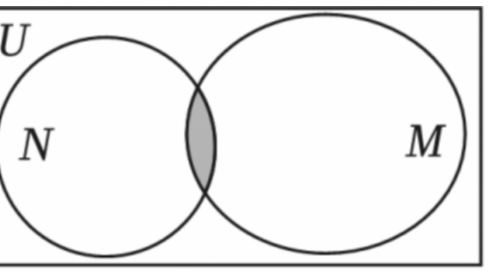
\includegraphics[width=0.30\textwidth]{figures/gao87_q14_venn.png}
\end{center}

\keepwithprev
A. $3$ 个\qquad B. $2$ 个\qquad C. $1$ 个\qquad D. 无穷多个

\ifanswer
\solbegin
\step{阴影部分所示的集合为 $M\cap N$，}
\step{$M=\{x\mid-1\leqslant x\leqslant3\}$，在此范围内的奇数有 $1$ 和 $3$，}
\step{所以集合 $M\cap N=\{1,3\}$ 共有 $2$ 个元素，故选 $B$.}
\solend
\fi

\item 已知实数 $a,b,c$ 满足 $a>b$，则下列不等式成立的是\mbox{（\quad）}

\keepwithprev
A. $-\dfrac1a<\dfrac1b$\qquad B. $a^2>b^2$\qquad C. $a\lvert c\rvert>b\lvert c\rvert$\qquad D. $\dfrac a{c^2+1}>\dfrac b{c^2+1}$

\ifanswer
\solbegin
\step{若 $a=1,b=-1$，则 $-1=-\dfrac1a=\dfrac1b=1$，$a^2=b^2=1$，则 AB 错误；}
\step{若 $a>b,c=0$，则 $a\lvert c\rvert=b\lvert c\rvert=0$，则 C 错误；}
\step{因为 $c^2+1\geqslant1$，所以 $0<\dfrac1{c^2+1}\leqslant1$，又 $a>b$，所以 $\dfrac a{c^2+1}>\dfrac b{c^2+1}$，}
\step{则 D 正确.}
\step{故选 $D$.}
\solend
\fi

\item 设集合 $P_1=\{x\mid x^2+ax+1>0\}$，$P_2=\{x\mid x^2+ax+2>0\}$，$Q_1=\{x\mid x^2+x+b>0\}$，
$Q_2=\{x\mid x^2+2x+b>0\}$，其中 $a$、$b\in\R$，下列说法中正确的是\mbox{（\quad）}

\keepwithprev
A. 对任意 $a$，$P_1$ 是 $P_2$ 的子集，对任意 $b$，$Q_1$ 不是 $Q_2$ 的子集

B. 对任意 $a$，$P_1$ 是 $P_2$ 的子集，存在 $b$，使得 $Q_1$ 是 $Q_2$ 的子集

C. 存在 $a$，使得 $P_1$ 不是 $P_2$ 的子集，对任意 $b$，$Q_1$ 不是 $Q_2$ 的子集

D. 存在 $a$，使得 $P_1$ 不是 $P_2$ 的子集，存在 $b$，使得 $Q_1$ 是 $Q_2$ 的子集

\ifanswer
\solbegin
\step{对于集合 $P_1=\{x\mid x^2+ax+1>0\}$，$P_2=\{x\mid x^2+ax+2>0\}$，}
\step{得当 $m\in P_1$ 时，即 $m^2+am+1>0$，得 $m^2+am+2>0$，}
\step{即有 $m\in P_2$，得对任意 $a$，$P_1$ 是 $P_2$ 的子集，}
\step{对于集合 $Q_1=\{x\mid x^2+x+b>0\}$，$Q_2=\{x\mid x^2+2x+b>0\}$，}
\step{当 $b=6$ 时，$Q_1=\{x\mid x^2+x+6>0\}=\R$，$Q_2=\{x\mid x^2+2x+6>0\}=\R$，}
\step{得 $Q_1$ 是 $Q_2$ 的子集，}
\step{当 $b=1$ 时，$Q_1=\{x\mid x^2+x+1>0\}=\R$，}
\step{$Q_2=\{x\mid x^2+2x+1>0\}=\{x\mid x\neq-1\}$，得 $Q_1$ 不是 $Q_2$ 的子集，}
\step{所以存在 $b$，使得 $Q_1$ 是 $Q_2$ 的子集，故选 $B$.}
\solend
\fi

\end{enumerate}

\bigsec{三、解答题}

\begin{enumerate}
\setcounter{enumi}{16}

\item 设 $m$ 为实数，求关于 $x$ 与 $y$ 的二元一次方程组 $\begin{cases}y=x+m\\ mx-y=4\end{cases}$ 的解集.

\ansspace*[8]

\ifanswer
\solbegin
\step{消去 $y$ 得 $(m-1)x=m+4$，}
\step{当 $m-1=0$，即 $m=1$ 时，$0=5$ 不成立，则 $x$ 无解，原方程组的解集为 $\varnothing$；}
\step{当 $m-1\neq0$，即 $m\neq1$ 时，则 $x=\dfrac{m+4}{m-1}$，$y=\dfrac{m+4}{m-1}+m=\dfrac{m^2+4}{m-1}$，}
\step{原方程组的解集为 $\left\{\left(\dfrac{m+4}{m-1},\dfrac{m^2+4}{m-1}\right)\right\}$.}
\step{综上所述，当 $m=1$ 时，方程组的解集为 $\varnothing$；}
\step{当 $m\neq1$ 时，方程组的解集为 $\left\{\left(\dfrac{m+4}{m-1},\dfrac{m^2+4}{m-1}\right)\right\}$.}
\solend
\fi

\item 设 $x<y<0$，试比较 $(x^2+y^2)(x-y)$ 与 $(x^2-y^2)(x+y)$ 的大小.

\ansspace*[9]

\ifanswer
\solbegin
\step{$(x^2+y^2)(x-y)-(x^2-y^2)(x+y)=(x-y)[x^2+y^2-(x+y)^2]=-2xy(x-y)$，}
\step{因为 $x<y<0$，所以 $xy>0$，$x-y<0$，所以 $-2xy(x-y)>0$，}
\step{即 $(x^2+y^2)(x-y)>(x^2-y^2)(x+y)$.}
\solend
\fi

\item 已知全集 $U=\R$，集合 $A=\left\{x\left|\dfrac{2+x}{3-x}>0\right.\right\}$，集合 $B=\{x\mid\lvert x-2\rvert>3\}$.

（1）求 $A\cup B$、$\overline A\cap B$.

（2）若集合 $C=\{x\mid x\leqslant a\}$，且 $A\cap C=A$，求实数 $a$ 的范围.

\ansspace*[10]

\ifanswer
\solbegin
\stepm{（1）}{由 $\lvert x-2\rvert>3$ 得 $x-2>3$ 或 $x-2<-3$，即 $x<-1$ 或 $x>5$，}
\step{所以 $B=(-\infty,-1)\cup(5,+\infty)$，}
\step{$A=\left\{x\left|\dfrac{2+x}{3-x}>0\right.\right\}=\{x\mid(2+x)(3-x)>0\}=(-2,3)$，}
\step{所以 $A\cup b=(-\infty,3)\cup(5m+\infty)$，}
\step{$\overline A=(-\infty,-2]\cup[3,+\infty)$，$\overline A\cap B=(-\infty,-2]\cup(5,+\infty)$.}
\stepm{（2）}{因为 $A\cap C=A$，所以 $A\subseteq C$，}
\step{因为 $A=(-2,3)$，所以实数 $a$ 的取值范围为 $\{a\mid a\geqslant3\}$.}
\solend
\fi

\item 已知函数 $f(x)=ax^2+4x+b\,(a<0,a,b\in\R)$，设关于 $x$ 的方程 $f(x)=0$ 的两实根为 $x_1$、
$x_2$，方程 $f(x)=x$ 的两实根为 $\alpha,\beta$.

（1）不等式 $f(x)<0$ 的解集是 $(-\infty,-3)\cup(5,+\infty)$，求不等式 $bx^2-ax-4<0$ 的解集；

（2）若 $a,b$ 均为负整数，且 $\lvert\alpha-\beta\rvert=1$，求 $f(x)$ 的解析式.

\ansspace*[12]

\ifanswer
\solbegin
\stepm{（1）}{$ax^2+4x+b<0$ 的解集为 $(-\infty,-3)\cup(5,+\infty)$，}
\step{所以 $-3,5$ 是方程 $ax^2+4x+b=0$ 的两根，所以 $\begin{cases}-3+5=-\dfrac4a\\ -3\times5=\dfrac ba\end{cases}\Rightarrow\begin{cases}a=-2\\ b=30\end{cases}$，}
\step{所以 $bx^2-ax-4<0$ 为 $30x^2+2x-4<0\Rightarrow15x^2+x-2<0$，}
\step{所以 $(3x-1)(5x+2)<0\Rightarrow-\dfrac25<x<\dfrac13$，}
\step{所以所求不等式的解集为 $\left\{x\left|-\dfrac25<x<\dfrac13\right.\right\}$.}
\stepm{（2）}{由题意得 $f(x)=ax^2+4x+b\,(a<0,a,b\in\R)$ 有两个不等实根为 $\alpha$、$\beta$，}
\step{所以 $\Delta=9-4ab>0$，$\alpha+\beta=-\dfrac3a$，$\alpha\beta=\dfrac ba$.}
\step{由 $\lvert\alpha-\beta\rvert=1$ 得 $(\alpha-\beta)^2=1$，即 $(\alpha+\beta)^2-4\alpha\beta=\dfrac9{a^2}-\dfrac{4b}a=1$，}
\step{所以 $9-4ab=a^2$，即 $a^2+4ab=9\,(a<0,a,b\in\R)$.}
\step{因为 $a,b$ 均为负整数，}
\step{所以 $\begin{cases}a=-1\\ a+4b=-9\end{cases}$ 或 $\begin{cases}a=-9\\ a+4b=-1\end{cases}$ 或 $\begin{cases}a=-3\\ a+4b=-3\end{cases}$，}
\step{显然后两种情况不合题意，应舍去，从而有 $\begin{cases}a=-1\\ a+4b=-9\end{cases}$，解得 $a=-1$，$b=-2$.}
\step{故所求函数解析式为 $f(x)=-x^2+4x-2$.}
\solend
\fi

\item 已知集合 $A=\{x\mid x=m^2+n^2,m\in\Z,n\in\Z\}$.

（1）判断 $2,5,25$ 是否属于集合 $A$；

（2）若正整数 $y$ 能表示为某个整数的平方，$z\in A$，证明：$yz\in A$；

（3）若集合 $B=\{x\mid x=4k+3,k\in\Z\}$，证明：$A\cap B=\varnothing$.

\ansspace*[14]

\ifanswer
\solbegin
\stepm{（1）}{由 $2=1^2+1^2$，$5=1^2+2^2$，$25=3^2+4^2$ 得 $2,5,25$ 属于集合 $A$；}
\stepm{（2）}{设 $y=a^2\,(a\in\Z)$，由 $z\in A$，设 $z=b^2+c^2\,(b\in\Z,c\in\Z)$，}
\step{则 $yz=a^2(b^2+c^2)=(ab)^2+(ac)^2$，}
\step{因为 $a\in\Z$，$b\in\Z$，$c\in\Z$，所以 $ab\in\Z$，$ac\in\Z$，所以 $yz\in A$；}
\stepm{（3）}{①当 $m$、$n$ 都为偶数时，设 $m=2k_1\,(k_1\in\Z)$，$n=2k_2\,(k_2\in\Z)$，}
\step{则 $x=m^2+n^2=4k_1^2+4k_2^2=4(k_1^2+k_2^2)$，此时 $x$ 为 $4$ 的倍数，}
\step{因为偶数 $\notin B$，所以 $A\cap B=\varnothing$；}
\step{②当 $m$、$n$ 都为奇数时，设 $m=2k_1+1\,(k_1\in\Z)$，$n=2k_2+1\,(k_2\in\Z)$，}
\step{则 $x=m^2+n^2=(2k_1+1)^2+(2k_2+1)^2=4(k_1^2+k_2^2+k_1+k_2)+2$，}
\step{此时 $x$ 为 $2$ 的倍数，因为偶数 $\notin B$，所以 $A\cap B=\varnothing$；}
\step{③当 $m$、$n$ 一奇一偶时，设 $m=2k_1+1\,(k_1\in\Z)$，$n=2k_2\,(k_2\in\Z)$，}
\step{则 $x=m^2+n^2=(2k_1+1)^2+(2k_2)^2=4(k_1^2+k_2^2+k_1)+1$，}
\step{此时 $x$ 被 $4$ 除余 $1$，而 $B$ 中元素被 $4$ 除余 $3$，此时 $A\cap B=\varnothing$.}
\step{综上，$A\cap B=\varnothing$.}
\solend
\fi

\end{enumerate}

\end{document}
"
% 紧凑版：xelatex "\def\iscompact{1}% 高一87_五十四中学_10月月考.tex
%   —— 高一上数学“2026-2027 年五十四中学高一上 10 月月考”（讲评版）
% 试卷版：xelatex 高一87_五十四中学_10月月考.tex
% 答案版：xelatex "\def\isanswer{1}% 高一87_五十四中学_10月月考.tex
%   —— 高一上数学“2026-2027 年五十四中学高一上 10 月月考”（讲评版）
% 试卷版：xelatex 高一87_五十四中学_10月月考.tex
% 答案版：xelatex "\def\isanswer{1}\input{高一87_五十四中学_10月月考.tex}"
% 紧凑版：xelatex "\def\iscompact{1}\input{高一87_五十四中学_10月月考.tex}"
%
% 原始材料：微信公众号“魔都数学加油站”文章，连载“27学年高一87”；
% 原文标题“27学年高一87——2026-2027年上海市五十四中学高一上10月月考”；
% 原文链接：https://mp.weixin.qq.com/s/pqPpSGQt0AhydcpaB8uEkQ。
% 页面标注发布时间 2026-10-27 17:43（上海）。
% 正文为 7 张 PNG 页（`原图/高一87_五十四中学_10月月考/01..07.png`），
% 尺寸混排（第 1、2 页为 4762×6735，第 3—7 页为 2560×3620），均按页序读取。
%
% 篇幅与题号：原卷自第 3 题起编号（第 1、2 题不在原文内）。填空题 3—12（10 题）、
% 选择题 13—16（4 题）、解答题 17—21（5 题），共 19 题。
%
% 讲评版：第 3、5、6 题只印【答案】（“$x\leqslant1$ 且 $y\leqslant1$”“$\{(2,6),(6,2)\}$”
% “$(-1,3]$”），本稿只给 \ans{}；其余 16 题印【解析】，其中选择题答案在解析末句
% “故选 A／B／D／B”。第 14 题题干带一幅韦恩图（裁自第 3 页原图、去粉色水印后转灰度），
% 三版都出。
%
% 副标题：原卷未印副标题。本稿按内容标作“集合与常用逻辑用语、不等式”。
%
% 原卷笔误/存疑（均照录未改，正文对应处另有 % 注）：
%   ① 第 19 题 (1) 解析作“所以 $A\cup b=(-\infty,3)\cup(5m+\infty)$”，两处均系排印错：
%      按上下文应为“$A\cup B=(-\infty,3)\cup(5,+\infty)$”（同页下一行 $\overline A\cap B$
%      的端点 $5$、$+\infty$ 也印证这一点）。原卷印作 $b$ 与 $5m+\infty$，照录未改。
%
% 与原卷的排版差异：
%   ① 原卷每题下直接印【答案】/【解析】，本稿按全稿惯例将答案与解析置于答案版；
%   ② 原卷未印副标题，本稿补出；填空横线统一排 \blankline[4.4em]；
%   ③ 原卷数集记号排斜体 $R$、$Z$、$N$，本稿按全稿惯例改用 $\R$、$\Z$、$\N$；
%   ④ 第 17—21 题的子问用行内“（1）（2）（3）”段，解析中的子问标号用 \stepm；
%   ⑤ 解答题按惯例加 \ansspace；选择题括号排 \mbox{（\quad）}。
%
% 行数核对：逐题数 \step/\stepm 条数，合计 86 条（Q4：1；Q7：4；Q8：2；Q9：2；Q10：3；
% Q11：9；Q12：3；Q13：2；Q14：3；Q15：5；Q16：9；Q17：6；Q18：3；Q19：7；Q20：13；
% Q21：14）；第 3、5、6 题只印【答案】，提 \ans{}，不计入 \step 账。原卷解析的换行
% 按语意合并，未逐行强拆。
%
\documentclass[a4paper,11pt]{article}
\usepackage{common}

\begin{document}

\examtitlest[7]{2026--2027 年五十四中学高一上 10 月月考}{集合与常用逻辑用语、不等式}

\bigsec{一、填空题}

\begin{enumerate}
\setcounter{enumi}{2}

\item “$x>1$ 或 $y>1$”的否定形式为\blankline[4.4em].

\ifanswer
\ans{$x\leqslant1$ 且 $y\leqslant1$}
\fi

\item 已知 $1<a<2$，$-3<b<3$，则 $a+b$ 的取值范围是\blankline[4.4em].

\ifanswer
\solbegin
\step{由不等式的可加性得 $-2<a+b<5$，故 $a+b$ 的取值范围是 $(-2,5)$.}
\solend
\fi

\item 方程组 $\begin{cases}x+y=8\\ xy=12\end{cases}$ 的解集为\blankline[4.4em].

\ifanswer
\ans{$\{(2,6),(6,2)\}$}
\fi

\item 不等式 $\dfrac{x-3}{x+1}\leqslant0$ 解集为\blankline[4.4em].

\ifanswer
\ans{$(-1,3]$}
\fi

\item 已知集合 $A=\{x\mid y=\sqrt{x+1}\}$，$B=\{y\mid y=x^2+5\}$，则 $A\cup B=\blankline[4.4em]$.

\ifanswer
\solbegin
\step{对于函数 $y=\sqrt{x+1}$，则 $x+1\geqslant0$，解得 $x\geqslant-1$，}
\step{所以 $A=\{x\mid y=\sqrt{x+1}\}=\{x\mid x\geqslant-1\}$，}
\step{因为 $x^2\geqslant0$，所以 $y=x^2+5\geqslant5$，所以 $B=\{y\mid y=x^2+5\}=\{y\mid y\geqslant5\}$，}
\step{所以 $A\cup B=\{x\mid x\geqslant-1\}$.}
\solend
\fi

\item 已知关于 $x$ 的不等式 $\lvert x+a\rvert<b$ 的解集为 $\{x\mid2<x<4\}$，则 $a+b$ 的值是\blankline[4.4em].

\ifanswer
\solbegin
\step{由 $\lvert x+a\rvert<b$，得 $-b-a<x<b-a$，则 $\begin{cases}-b-a=2\\ b-a=4\end{cases}$，解得 $a=-3$，$b=1$，}
\step{所以 $a+b=-2$.}
\solend
\fi

\item 已知一元二次方程 $x^2-2mx+m-1=0$ 的两实根为 $x_1,x_2$，且 $x_1^2+x_2^2=4$，则实数 $m$ 的值
是\blankline[4.4em].

\ifanswer
\solbegin
\step{由题意得 $x_1+x_2=2m$，$x_1x_2=m-1$，}
\step{所以 $x_1^2+x_2^2=(x_1+x_2)^2-2x_1x_2=4m^2-2m+2=4$，解得 $m=1$ 或 $m=-\dfrac12$.}
\solend
\fi

\item 已知集合 $A=\{x\mid x^2-x-6=0\}$，$B=\{y\mid ay-1=0\}$，若 $A\cap B=B$，则实数
$a=\blankline[4.4em]$.

\ifanswer
\solbegin
\step{$A=\{-2,3\}$，由 $A\cap B=B$，得 $B\subseteq A$，而 $B=\{y\mid ay-1=0\}$，}
\step{则当 $B=\varnothing$ 时，$a=0$；当 $B=\{-2\}$ 时，$-2a-1=0$，解得 $a=-\dfrac12$；}
\step{当 $B=\{3\}$ 时，$3a-1=0$，解得 $a=\dfrac13$，所以实数 $a$ 的值为 $-\dfrac12$ 或 $0$ 或 $\dfrac13$.}
\solend
\fi

\item 已知集合 $A=\{x\mid(m-1)x^2+(m-1)x+2\leqslant0,x\in\R\}$，$B=\left\{x\left|\dfrac{2x-1}{x^2+x+1}>1,x\in\R\right.\right\}$，
且 $A\cap B=A$，则实数 $m$ 的取值范围是\blankline[4.4em].

\ifanswer
\solbegin
\step{因为 $\dfrac{2x-1}{x^2+x+1}>1$，所以 $x^2-x+2<0$，显然不等式无解，}
\step{所以 $B=\left\{x\left|\dfrac{2x-1}{x^2+x+1}>1,x\in\R\right.\right\}=\varnothing$，而 $A\cap B=A$，则 $A=\varnothing$，}
\step{①当 $m=1$ 时，$2\leqslant0$ 不成立，此时 $A=\varnothing$，}
\step{②当 $m<1$ 时，$m-1<0$，函数 $y=(m-1)x^2+(m-1)x+2$，开口向下，}
\step{不等式 $(m-1)x^2+(m-1)x+2\leqslant0$ 有解，$A\neq\varnothing$，}
\step{③当 $m>1$ 时，函数 $y=(m-1)x^2+(m-1)x+2$，开口向上，}
\step{若不等式 $(m-1)x^2+(m-1)x+2\leqslant0$ 无解，}
\step{只需 $\Delta=(m-1)^2-8(m-1)<0$，解得 $1<m<9$，}
\step{综上，$m$ 的取值范围是 $[1,9]$.}
\solend
\fi

\item 设 $A$ 是整数集的一个非空子集，对于 $k\in A$，如果 $k-1\notin A$ 且 $k+1\notin A$，那么 $k$ 是 $A$
的一个“孤立元”. 给定 $S=\{1,2,3,4,5,6,7,8\}$，由 $S$ 的 $3$ 个元素构成的所有集合中，不含
“孤立元”的集合共有\blankline[3.6em]个.

\ifanswer
\solbegin
\step{由题意得，“孤立元”即为在集合中无与之相邻的元素，}
\step{满足条件的集合有 $\{1,2,3\},\{2,3,4\},\{3,4,5\},\{4,5,6\},\{5,6,7\},\{6,7,8\}$，}
\step{共 $6$ 个集合.}
\solend
\fi

\end{enumerate}

\bigsec{二、选择题}

\begin{enumerate}
\setcounter{enumi}{12}

\item “$m=2$”是“$m^2=4$”的\mbox{（\quad）}条件.

\keepwithprev
A. 充分非必要条件\qquad B. 必要非充分条件

C. 充要条件\qquad D. 既非充分又非必要条件

\ifanswer
\solbegin
\step{由 $m^2=4$，解得 $m=\pm2$，故“$m=2$”是“$m^2=4$”的充分不必要条件，}
\step{故选 $A$.}
\solend
\fi

\item 已知全集 $U=\R$，集合 $M=\{x\mid\lvert x-1\rvert\leqslant2\}$ 和 $N=\{x\mid x=2k-1,k\in\Z\}$ 的关系
的韦恩（$Venn$）图如图所示，则阴影部分所示的集合的元素共有\mbox{（\quad）}

\begin{center}
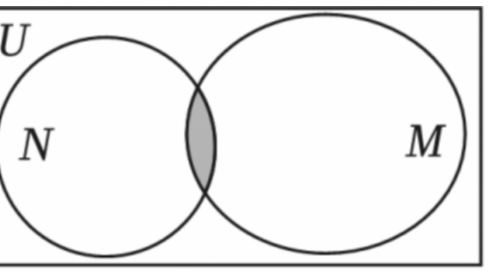
\includegraphics[width=0.30\textwidth]{figures/gao87_q14_venn.png}
\end{center}

\keepwithprev
A. $3$ 个\qquad B. $2$ 个\qquad C. $1$ 个\qquad D. 无穷多个

\ifanswer
\solbegin
\step{阴影部分所示的集合为 $M\cap N$，}
\step{$M=\{x\mid-1\leqslant x\leqslant3\}$，在此范围内的奇数有 $1$ 和 $3$，}
\step{所以集合 $M\cap N=\{1,3\}$ 共有 $2$ 个元素，故选 $B$.}
\solend
\fi

\item 已知实数 $a,b,c$ 满足 $a>b$，则下列不等式成立的是\mbox{（\quad）}

\keepwithprev
A. $-\dfrac1a<\dfrac1b$\qquad B. $a^2>b^2$\qquad C. $a\lvert c\rvert>b\lvert c\rvert$\qquad D. $\dfrac a{c^2+1}>\dfrac b{c^2+1}$

\ifanswer
\solbegin
\step{若 $a=1,b=-1$，则 $-1=-\dfrac1a=\dfrac1b=1$，$a^2=b^2=1$，则 AB 错误；}
\step{若 $a>b,c=0$，则 $a\lvert c\rvert=b\lvert c\rvert=0$，则 C 错误；}
\step{因为 $c^2+1\geqslant1$，所以 $0<\dfrac1{c^2+1}\leqslant1$，又 $a>b$，所以 $\dfrac a{c^2+1}>\dfrac b{c^2+1}$，}
\step{则 D 正确.}
\step{故选 $D$.}
\solend
\fi

\item 设集合 $P_1=\{x\mid x^2+ax+1>0\}$，$P_2=\{x\mid x^2+ax+2>0\}$，$Q_1=\{x\mid x^2+x+b>0\}$，
$Q_2=\{x\mid x^2+2x+b>0\}$，其中 $a$、$b\in\R$，下列说法中正确的是\mbox{（\quad）}

\keepwithprev
A. 对任意 $a$，$P_1$ 是 $P_2$ 的子集，对任意 $b$，$Q_1$ 不是 $Q_2$ 的子集

B. 对任意 $a$，$P_1$ 是 $P_2$ 的子集，存在 $b$，使得 $Q_1$ 是 $Q_2$ 的子集

C. 存在 $a$，使得 $P_1$ 不是 $P_2$ 的子集，对任意 $b$，$Q_1$ 不是 $Q_2$ 的子集

D. 存在 $a$，使得 $P_1$ 不是 $P_2$ 的子集，存在 $b$，使得 $Q_1$ 是 $Q_2$ 的子集

\ifanswer
\solbegin
\step{对于集合 $P_1=\{x\mid x^2+ax+1>0\}$，$P_2=\{x\mid x^2+ax+2>0\}$，}
\step{得当 $m\in P_1$ 时，即 $m^2+am+1>0$，得 $m^2+am+2>0$，}
\step{即有 $m\in P_2$，得对任意 $a$，$P_1$ 是 $P_2$ 的子集，}
\step{对于集合 $Q_1=\{x\mid x^2+x+b>0\}$，$Q_2=\{x\mid x^2+2x+b>0\}$，}
\step{当 $b=6$ 时，$Q_1=\{x\mid x^2+x+6>0\}=\R$，$Q_2=\{x\mid x^2+2x+6>0\}=\R$，}
\step{得 $Q_1$ 是 $Q_2$ 的子集，}
\step{当 $b=1$ 时，$Q_1=\{x\mid x^2+x+1>0\}=\R$，}
\step{$Q_2=\{x\mid x^2+2x+1>0\}=\{x\mid x\neq-1\}$，得 $Q_1$ 不是 $Q_2$ 的子集，}
\step{所以存在 $b$，使得 $Q_1$ 是 $Q_2$ 的子集，故选 $B$.}
\solend
\fi

\end{enumerate}

\bigsec{三、解答题}

\begin{enumerate}
\setcounter{enumi}{16}

\item 设 $m$ 为实数，求关于 $x$ 与 $y$ 的二元一次方程组 $\begin{cases}y=x+m\\ mx-y=4\end{cases}$ 的解集.

\ansspace*[8]

\ifanswer
\solbegin
\step{消去 $y$ 得 $(m-1)x=m+4$，}
\step{当 $m-1=0$，即 $m=1$ 时，$0=5$ 不成立，则 $x$ 无解，原方程组的解集为 $\varnothing$；}
\step{当 $m-1\neq0$，即 $m\neq1$ 时，则 $x=\dfrac{m+4}{m-1}$，$y=\dfrac{m+4}{m-1}+m=\dfrac{m^2+4}{m-1}$，}
\step{原方程组的解集为 $\left\{\left(\dfrac{m+4}{m-1},\dfrac{m^2+4}{m-1}\right)\right\}$.}
\step{综上所述，当 $m=1$ 时，方程组的解集为 $\varnothing$；}
\step{当 $m\neq1$ 时，方程组的解集为 $\left\{\left(\dfrac{m+4}{m-1},\dfrac{m^2+4}{m-1}\right)\right\}$.}
\solend
\fi

\item 设 $x<y<0$，试比较 $(x^2+y^2)(x-y)$ 与 $(x^2-y^2)(x+y)$ 的大小.

\ansspace*[9]

\ifanswer
\solbegin
\step{$(x^2+y^2)(x-y)-(x^2-y^2)(x+y)=(x-y)[x^2+y^2-(x+y)^2]=-2xy(x-y)$，}
\step{因为 $x<y<0$，所以 $xy>0$，$x-y<0$，所以 $-2xy(x-y)>0$，}
\step{即 $(x^2+y^2)(x-y)>(x^2-y^2)(x+y)$.}
\solend
\fi

\item 已知全集 $U=\R$，集合 $A=\left\{x\left|\dfrac{2+x}{3-x}>0\right.\right\}$，集合 $B=\{x\mid\lvert x-2\rvert>3\}$.

（1）求 $A\cup B$、$\overline A\cap B$.

（2）若集合 $C=\{x\mid x\leqslant a\}$，且 $A\cap C=A$，求实数 $a$ 的范围.

\ansspace*[10]

\ifanswer
\solbegin
\stepm{（1）}{由 $\lvert x-2\rvert>3$ 得 $x-2>3$ 或 $x-2<-3$，即 $x<-1$ 或 $x>5$，}
\step{所以 $B=(-\infty,-1)\cup(5,+\infty)$，}
\step{$A=\left\{x\left|\dfrac{2+x}{3-x}>0\right.\right\}=\{x\mid(2+x)(3-x)>0\}=(-2,3)$，}
\step{所以 $A\cup b=(-\infty,3)\cup(5m+\infty)$，}
\step{$\overline A=(-\infty,-2]\cup[3,+\infty)$，$\overline A\cap B=(-\infty,-2]\cup(5,+\infty)$.}
\stepm{（2）}{因为 $A\cap C=A$，所以 $A\subseteq C$，}
\step{因为 $A=(-2,3)$，所以实数 $a$ 的取值范围为 $\{a\mid a\geqslant3\}$.}
\solend
\fi

\item 已知函数 $f(x)=ax^2+4x+b\,(a<0,a,b\in\R)$，设关于 $x$ 的方程 $f(x)=0$ 的两实根为 $x_1$、
$x_2$，方程 $f(x)=x$ 的两实根为 $\alpha,\beta$.

（1）不等式 $f(x)<0$ 的解集是 $(-\infty,-3)\cup(5,+\infty)$，求不等式 $bx^2-ax-4<0$ 的解集；

（2）若 $a,b$ 均为负整数，且 $\lvert\alpha-\beta\rvert=1$，求 $f(x)$ 的解析式.

\ansspace*[12]

\ifanswer
\solbegin
\stepm{（1）}{$ax^2+4x+b<0$ 的解集为 $(-\infty,-3)\cup(5,+\infty)$，}
\step{所以 $-3,5$ 是方程 $ax^2+4x+b=0$ 的两根，所以 $\begin{cases}-3+5=-\dfrac4a\\ -3\times5=\dfrac ba\end{cases}\Rightarrow\begin{cases}a=-2\\ b=30\end{cases}$，}
\step{所以 $bx^2-ax-4<0$ 为 $30x^2+2x-4<0\Rightarrow15x^2+x-2<0$，}
\step{所以 $(3x-1)(5x+2)<0\Rightarrow-\dfrac25<x<\dfrac13$，}
\step{所以所求不等式的解集为 $\left\{x\left|-\dfrac25<x<\dfrac13\right.\right\}$.}
\stepm{（2）}{由题意得 $f(x)=ax^2+4x+b\,(a<0,a,b\in\R)$ 有两个不等实根为 $\alpha$、$\beta$，}
\step{所以 $\Delta=9-4ab>0$，$\alpha+\beta=-\dfrac3a$，$\alpha\beta=\dfrac ba$.}
\step{由 $\lvert\alpha-\beta\rvert=1$ 得 $(\alpha-\beta)^2=1$，即 $(\alpha+\beta)^2-4\alpha\beta=\dfrac9{a^2}-\dfrac{4b}a=1$，}
\step{所以 $9-4ab=a^2$，即 $a^2+4ab=9\,(a<0,a,b\in\R)$.}
\step{因为 $a,b$ 均为负整数，}
\step{所以 $\begin{cases}a=-1\\ a+4b=-9\end{cases}$ 或 $\begin{cases}a=-9\\ a+4b=-1\end{cases}$ 或 $\begin{cases}a=-3\\ a+4b=-3\end{cases}$，}
\step{显然后两种情况不合题意，应舍去，从而有 $\begin{cases}a=-1\\ a+4b=-9\end{cases}$，解得 $a=-1$，$b=-2$.}
\step{故所求函数解析式为 $f(x)=-x^2+4x-2$.}
\solend
\fi

\item 已知集合 $A=\{x\mid x=m^2+n^2,m\in\Z,n\in\Z\}$.

（1）判断 $2,5,25$ 是否属于集合 $A$；

（2）若正整数 $y$ 能表示为某个整数的平方，$z\in A$，证明：$yz\in A$；

（3）若集合 $B=\{x\mid x=4k+3,k\in\Z\}$，证明：$A\cap B=\varnothing$.

\ansspace*[14]

\ifanswer
\solbegin
\stepm{（1）}{由 $2=1^2+1^2$，$5=1^2+2^2$，$25=3^2+4^2$ 得 $2,5,25$ 属于集合 $A$；}
\stepm{（2）}{设 $y=a^2\,(a\in\Z)$，由 $z\in A$，设 $z=b^2+c^2\,(b\in\Z,c\in\Z)$，}
\step{则 $yz=a^2(b^2+c^2)=(ab)^2+(ac)^2$，}
\step{因为 $a\in\Z$，$b\in\Z$，$c\in\Z$，所以 $ab\in\Z$，$ac\in\Z$，所以 $yz\in A$；}
\stepm{（3）}{①当 $m$、$n$ 都为偶数时，设 $m=2k_1\,(k_1\in\Z)$，$n=2k_2\,(k_2\in\Z)$，}
\step{则 $x=m^2+n^2=4k_1^2+4k_2^2=4(k_1^2+k_2^2)$，此时 $x$ 为 $4$ 的倍数，}
\step{因为偶数 $\notin B$，所以 $A\cap B=\varnothing$；}
\step{②当 $m$、$n$ 都为奇数时，设 $m=2k_1+1\,(k_1\in\Z)$，$n=2k_2+1\,(k_2\in\Z)$，}
\step{则 $x=m^2+n^2=(2k_1+1)^2+(2k_2+1)^2=4(k_1^2+k_2^2+k_1+k_2)+2$，}
\step{此时 $x$ 为 $2$ 的倍数，因为偶数 $\notin B$，所以 $A\cap B=\varnothing$；}
\step{③当 $m$、$n$ 一奇一偶时，设 $m=2k_1+1\,(k_1\in\Z)$，$n=2k_2\,(k_2\in\Z)$，}
\step{则 $x=m^2+n^2=(2k_1+1)^2+(2k_2)^2=4(k_1^2+k_2^2+k_1)+1$，}
\step{此时 $x$ 被 $4$ 除余 $1$，而 $B$ 中元素被 $4$ 除余 $3$，此时 $A\cap B=\varnothing$.}
\step{综上，$A\cap B=\varnothing$.}
\solend
\fi

\end{enumerate}

\end{document}
"
% 紧凑版：xelatex "\def\iscompact{1}% 高一87_五十四中学_10月月考.tex
%   —— 高一上数学“2026-2027 年五十四中学高一上 10 月月考”（讲评版）
% 试卷版：xelatex 高一87_五十四中学_10月月考.tex
% 答案版：xelatex "\def\isanswer{1}\input{高一87_五十四中学_10月月考.tex}"
% 紧凑版：xelatex "\def\iscompact{1}\input{高一87_五十四中学_10月月考.tex}"
%
% 原始材料：微信公众号“魔都数学加油站”文章，连载“27学年高一87”；
% 原文标题“27学年高一87——2026-2027年上海市五十四中学高一上10月月考”；
% 原文链接：https://mp.weixin.qq.com/s/pqPpSGQt0AhydcpaB8uEkQ。
% 页面标注发布时间 2026-10-27 17:43（上海）。
% 正文为 7 张 PNG 页（`原图/高一87_五十四中学_10月月考/01..07.png`），
% 尺寸混排（第 1、2 页为 4762×6735，第 3—7 页为 2560×3620），均按页序读取。
%
% 篇幅与题号：原卷自第 3 题起编号（第 1、2 题不在原文内）。填空题 3—12（10 题）、
% 选择题 13—16（4 题）、解答题 17—21（5 题），共 19 题。
%
% 讲评版：第 3、5、6 题只印【答案】（“$x\leqslant1$ 且 $y\leqslant1$”“$\{(2,6),(6,2)\}$”
% “$(-1,3]$”），本稿只给 \ans{}；其余 16 题印【解析】，其中选择题答案在解析末句
% “故选 A／B／D／B”。第 14 题题干带一幅韦恩图（裁自第 3 页原图、去粉色水印后转灰度），
% 三版都出。
%
% 副标题：原卷未印副标题。本稿按内容标作“集合与常用逻辑用语、不等式”。
%
% 原卷笔误/存疑（均照录未改，正文对应处另有 % 注）：
%   ① 第 19 题 (1) 解析作“所以 $A\cup b=(-\infty,3)\cup(5m+\infty)$”，两处均系排印错：
%      按上下文应为“$A\cup B=(-\infty,3)\cup(5,+\infty)$”（同页下一行 $\overline A\cap B$
%      的端点 $5$、$+\infty$ 也印证这一点）。原卷印作 $b$ 与 $5m+\infty$，照录未改。
%
% 与原卷的排版差异：
%   ① 原卷每题下直接印【答案】/【解析】，本稿按全稿惯例将答案与解析置于答案版；
%   ② 原卷未印副标题，本稿补出；填空横线统一排 \blankline[4.4em]；
%   ③ 原卷数集记号排斜体 $R$、$Z$、$N$，本稿按全稿惯例改用 $\R$、$\Z$、$\N$；
%   ④ 第 17—21 题的子问用行内“（1）（2）（3）”段，解析中的子问标号用 \stepm；
%   ⑤ 解答题按惯例加 \ansspace；选择题括号排 \mbox{（\quad）}。
%
% 行数核对：逐题数 \step/\stepm 条数，合计 86 条（Q4：1；Q7：4；Q8：2；Q9：2；Q10：3；
% Q11：9；Q12：3；Q13：2；Q14：3；Q15：5；Q16：9；Q17：6；Q18：3；Q19：7；Q20：13；
% Q21：14）；第 3、5、6 题只印【答案】，提 \ans{}，不计入 \step 账。原卷解析的换行
% 按语意合并，未逐行强拆。
%
\documentclass[a4paper,11pt]{article}
\usepackage{common}

\begin{document}

\examtitlest[7]{2026--2027 年五十四中学高一上 10 月月考}{集合与常用逻辑用语、不等式}

\bigsec{一、填空题}

\begin{enumerate}
\setcounter{enumi}{2}

\item “$x>1$ 或 $y>1$”的否定形式为\blankline[4.4em].

\ifanswer
\ans{$x\leqslant1$ 且 $y\leqslant1$}
\fi

\item 已知 $1<a<2$，$-3<b<3$，则 $a+b$ 的取值范围是\blankline[4.4em].

\ifanswer
\solbegin
\step{由不等式的可加性得 $-2<a+b<5$，故 $a+b$ 的取值范围是 $(-2,5)$.}
\solend
\fi

\item 方程组 $\begin{cases}x+y=8\\ xy=12\end{cases}$ 的解集为\blankline[4.4em].

\ifanswer
\ans{$\{(2,6),(6,2)\}$}
\fi

\item 不等式 $\dfrac{x-3}{x+1}\leqslant0$ 解集为\blankline[4.4em].

\ifanswer
\ans{$(-1,3]$}
\fi

\item 已知集合 $A=\{x\mid y=\sqrt{x+1}\}$，$B=\{y\mid y=x^2+5\}$，则 $A\cup B=\blankline[4.4em]$.

\ifanswer
\solbegin
\step{对于函数 $y=\sqrt{x+1}$，则 $x+1\geqslant0$，解得 $x\geqslant-1$，}
\step{所以 $A=\{x\mid y=\sqrt{x+1}\}=\{x\mid x\geqslant-1\}$，}
\step{因为 $x^2\geqslant0$，所以 $y=x^2+5\geqslant5$，所以 $B=\{y\mid y=x^2+5\}=\{y\mid y\geqslant5\}$，}
\step{所以 $A\cup B=\{x\mid x\geqslant-1\}$.}
\solend
\fi

\item 已知关于 $x$ 的不等式 $\lvert x+a\rvert<b$ 的解集为 $\{x\mid2<x<4\}$，则 $a+b$ 的值是\blankline[4.4em].

\ifanswer
\solbegin
\step{由 $\lvert x+a\rvert<b$，得 $-b-a<x<b-a$，则 $\begin{cases}-b-a=2\\ b-a=4\end{cases}$，解得 $a=-3$，$b=1$，}
\step{所以 $a+b=-2$.}
\solend
\fi

\item 已知一元二次方程 $x^2-2mx+m-1=0$ 的两实根为 $x_1,x_2$，且 $x_1^2+x_2^2=4$，则实数 $m$ 的值
是\blankline[4.4em].

\ifanswer
\solbegin
\step{由题意得 $x_1+x_2=2m$，$x_1x_2=m-1$，}
\step{所以 $x_1^2+x_2^2=(x_1+x_2)^2-2x_1x_2=4m^2-2m+2=4$，解得 $m=1$ 或 $m=-\dfrac12$.}
\solend
\fi

\item 已知集合 $A=\{x\mid x^2-x-6=0\}$，$B=\{y\mid ay-1=0\}$，若 $A\cap B=B$，则实数
$a=\blankline[4.4em]$.

\ifanswer
\solbegin
\step{$A=\{-2,3\}$，由 $A\cap B=B$，得 $B\subseteq A$，而 $B=\{y\mid ay-1=0\}$，}
\step{则当 $B=\varnothing$ 时，$a=0$；当 $B=\{-2\}$ 时，$-2a-1=0$，解得 $a=-\dfrac12$；}
\step{当 $B=\{3\}$ 时，$3a-1=0$，解得 $a=\dfrac13$，所以实数 $a$ 的值为 $-\dfrac12$ 或 $0$ 或 $\dfrac13$.}
\solend
\fi

\item 已知集合 $A=\{x\mid(m-1)x^2+(m-1)x+2\leqslant0,x\in\R\}$，$B=\left\{x\left|\dfrac{2x-1}{x^2+x+1}>1,x\in\R\right.\right\}$，
且 $A\cap B=A$，则实数 $m$ 的取值范围是\blankline[4.4em].

\ifanswer
\solbegin
\step{因为 $\dfrac{2x-1}{x^2+x+1}>1$，所以 $x^2-x+2<0$，显然不等式无解，}
\step{所以 $B=\left\{x\left|\dfrac{2x-1}{x^2+x+1}>1,x\in\R\right.\right\}=\varnothing$，而 $A\cap B=A$，则 $A=\varnothing$，}
\step{①当 $m=1$ 时，$2\leqslant0$ 不成立，此时 $A=\varnothing$，}
\step{②当 $m<1$ 时，$m-1<0$，函数 $y=(m-1)x^2+(m-1)x+2$，开口向下，}
\step{不等式 $(m-1)x^2+(m-1)x+2\leqslant0$ 有解，$A\neq\varnothing$，}
\step{③当 $m>1$ 时，函数 $y=(m-1)x^2+(m-1)x+2$，开口向上，}
\step{若不等式 $(m-1)x^2+(m-1)x+2\leqslant0$ 无解，}
\step{只需 $\Delta=(m-1)^2-8(m-1)<0$，解得 $1<m<9$，}
\step{综上，$m$ 的取值范围是 $[1,9]$.}
\solend
\fi

\item 设 $A$ 是整数集的一个非空子集，对于 $k\in A$，如果 $k-1\notin A$ 且 $k+1\notin A$，那么 $k$ 是 $A$
的一个“孤立元”. 给定 $S=\{1,2,3,4,5,6,7,8\}$，由 $S$ 的 $3$ 个元素构成的所有集合中，不含
“孤立元”的集合共有\blankline[3.6em]个.

\ifanswer
\solbegin
\step{由题意得，“孤立元”即为在集合中无与之相邻的元素，}
\step{满足条件的集合有 $\{1,2,3\},\{2,3,4\},\{3,4,5\},\{4,5,6\},\{5,6,7\},\{6,7,8\}$，}
\step{共 $6$ 个集合.}
\solend
\fi

\end{enumerate}

\bigsec{二、选择题}

\begin{enumerate}
\setcounter{enumi}{12}

\item “$m=2$”是“$m^2=4$”的\mbox{（\quad）}条件.

\keepwithprev
A. 充分非必要条件\qquad B. 必要非充分条件

C. 充要条件\qquad D. 既非充分又非必要条件

\ifanswer
\solbegin
\step{由 $m^2=4$，解得 $m=\pm2$，故“$m=2$”是“$m^2=4$”的充分不必要条件，}
\step{故选 $A$.}
\solend
\fi

\item 已知全集 $U=\R$，集合 $M=\{x\mid\lvert x-1\rvert\leqslant2\}$ 和 $N=\{x\mid x=2k-1,k\in\Z\}$ 的关系
的韦恩（$Venn$）图如图所示，则阴影部分所示的集合的元素共有\mbox{（\quad）}

\begin{center}
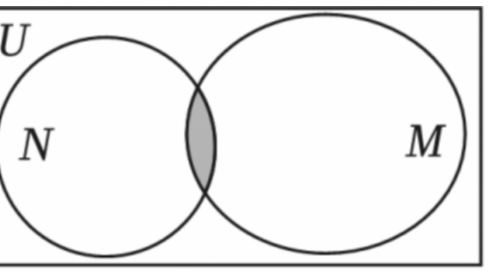
\includegraphics[width=0.30\textwidth]{figures/gao87_q14_venn.png}
\end{center}

\keepwithprev
A. $3$ 个\qquad B. $2$ 个\qquad C. $1$ 个\qquad D. 无穷多个

\ifanswer
\solbegin
\step{阴影部分所示的集合为 $M\cap N$，}
\step{$M=\{x\mid-1\leqslant x\leqslant3\}$，在此范围内的奇数有 $1$ 和 $3$，}
\step{所以集合 $M\cap N=\{1,3\}$ 共有 $2$ 个元素，故选 $B$.}
\solend
\fi

\item 已知实数 $a,b,c$ 满足 $a>b$，则下列不等式成立的是\mbox{（\quad）}

\keepwithprev
A. $-\dfrac1a<\dfrac1b$\qquad B. $a^2>b^2$\qquad C. $a\lvert c\rvert>b\lvert c\rvert$\qquad D. $\dfrac a{c^2+1}>\dfrac b{c^2+1}$

\ifanswer
\solbegin
\step{若 $a=1,b=-1$，则 $-1=-\dfrac1a=\dfrac1b=1$，$a^2=b^2=1$，则 AB 错误；}
\step{若 $a>b,c=0$，则 $a\lvert c\rvert=b\lvert c\rvert=0$，则 C 错误；}
\step{因为 $c^2+1\geqslant1$，所以 $0<\dfrac1{c^2+1}\leqslant1$，又 $a>b$，所以 $\dfrac a{c^2+1}>\dfrac b{c^2+1}$，}
\step{则 D 正确.}
\step{故选 $D$.}
\solend
\fi

\item 设集合 $P_1=\{x\mid x^2+ax+1>0\}$，$P_2=\{x\mid x^2+ax+2>0\}$，$Q_1=\{x\mid x^2+x+b>0\}$，
$Q_2=\{x\mid x^2+2x+b>0\}$，其中 $a$、$b\in\R$，下列说法中正确的是\mbox{（\quad）}

\keepwithprev
A. 对任意 $a$，$P_1$ 是 $P_2$ 的子集，对任意 $b$，$Q_1$ 不是 $Q_2$ 的子集

B. 对任意 $a$，$P_1$ 是 $P_2$ 的子集，存在 $b$，使得 $Q_1$ 是 $Q_2$ 的子集

C. 存在 $a$，使得 $P_1$ 不是 $P_2$ 的子集，对任意 $b$，$Q_1$ 不是 $Q_2$ 的子集

D. 存在 $a$，使得 $P_1$ 不是 $P_2$ 的子集，存在 $b$，使得 $Q_1$ 是 $Q_2$ 的子集

\ifanswer
\solbegin
\step{对于集合 $P_1=\{x\mid x^2+ax+1>0\}$，$P_2=\{x\mid x^2+ax+2>0\}$，}
\step{得当 $m\in P_1$ 时，即 $m^2+am+1>0$，得 $m^2+am+2>0$，}
\step{即有 $m\in P_2$，得对任意 $a$，$P_1$ 是 $P_2$ 的子集，}
\step{对于集合 $Q_1=\{x\mid x^2+x+b>0\}$，$Q_2=\{x\mid x^2+2x+b>0\}$，}
\step{当 $b=6$ 时，$Q_1=\{x\mid x^2+x+6>0\}=\R$，$Q_2=\{x\mid x^2+2x+6>0\}=\R$，}
\step{得 $Q_1$ 是 $Q_2$ 的子集，}
\step{当 $b=1$ 时，$Q_1=\{x\mid x^2+x+1>0\}=\R$，}
\step{$Q_2=\{x\mid x^2+2x+1>0\}=\{x\mid x\neq-1\}$，得 $Q_1$ 不是 $Q_2$ 的子集，}
\step{所以存在 $b$，使得 $Q_1$ 是 $Q_2$ 的子集，故选 $B$.}
\solend
\fi

\end{enumerate}

\bigsec{三、解答题}

\begin{enumerate}
\setcounter{enumi}{16}

\item 设 $m$ 为实数，求关于 $x$ 与 $y$ 的二元一次方程组 $\begin{cases}y=x+m\\ mx-y=4\end{cases}$ 的解集.

\ansspace*[8]

\ifanswer
\solbegin
\step{消去 $y$ 得 $(m-1)x=m+4$，}
\step{当 $m-1=0$，即 $m=1$ 时，$0=5$ 不成立，则 $x$ 无解，原方程组的解集为 $\varnothing$；}
\step{当 $m-1\neq0$，即 $m\neq1$ 时，则 $x=\dfrac{m+4}{m-1}$，$y=\dfrac{m+4}{m-1}+m=\dfrac{m^2+4}{m-1}$，}
\step{原方程组的解集为 $\left\{\left(\dfrac{m+4}{m-1},\dfrac{m^2+4}{m-1}\right)\right\}$.}
\step{综上所述，当 $m=1$ 时，方程组的解集为 $\varnothing$；}
\step{当 $m\neq1$ 时，方程组的解集为 $\left\{\left(\dfrac{m+4}{m-1},\dfrac{m^2+4}{m-1}\right)\right\}$.}
\solend
\fi

\item 设 $x<y<0$，试比较 $(x^2+y^2)(x-y)$ 与 $(x^2-y^2)(x+y)$ 的大小.

\ansspace*[9]

\ifanswer
\solbegin
\step{$(x^2+y^2)(x-y)-(x^2-y^2)(x+y)=(x-y)[x^2+y^2-(x+y)^2]=-2xy(x-y)$，}
\step{因为 $x<y<0$，所以 $xy>0$，$x-y<0$，所以 $-2xy(x-y)>0$，}
\step{即 $(x^2+y^2)(x-y)>(x^2-y^2)(x+y)$.}
\solend
\fi

\item 已知全集 $U=\R$，集合 $A=\left\{x\left|\dfrac{2+x}{3-x}>0\right.\right\}$，集合 $B=\{x\mid\lvert x-2\rvert>3\}$.

（1）求 $A\cup B$、$\overline A\cap B$.

（2）若集合 $C=\{x\mid x\leqslant a\}$，且 $A\cap C=A$，求实数 $a$ 的范围.

\ansspace*[10]

\ifanswer
\solbegin
\stepm{（1）}{由 $\lvert x-2\rvert>3$ 得 $x-2>3$ 或 $x-2<-3$，即 $x<-1$ 或 $x>5$，}
\step{所以 $B=(-\infty,-1)\cup(5,+\infty)$，}
\step{$A=\left\{x\left|\dfrac{2+x}{3-x}>0\right.\right\}=\{x\mid(2+x)(3-x)>0\}=(-2,3)$，}
\step{所以 $A\cup b=(-\infty,3)\cup(5m+\infty)$，}
\step{$\overline A=(-\infty,-2]\cup[3,+\infty)$，$\overline A\cap B=(-\infty,-2]\cup(5,+\infty)$.}
\stepm{（2）}{因为 $A\cap C=A$，所以 $A\subseteq C$，}
\step{因为 $A=(-2,3)$，所以实数 $a$ 的取值范围为 $\{a\mid a\geqslant3\}$.}
\solend
\fi

\item 已知函数 $f(x)=ax^2+4x+b\,(a<0,a,b\in\R)$，设关于 $x$ 的方程 $f(x)=0$ 的两实根为 $x_1$、
$x_2$，方程 $f(x)=x$ 的两实根为 $\alpha,\beta$.

（1）不等式 $f(x)<0$ 的解集是 $(-\infty,-3)\cup(5,+\infty)$，求不等式 $bx^2-ax-4<0$ 的解集；

（2）若 $a,b$ 均为负整数，且 $\lvert\alpha-\beta\rvert=1$，求 $f(x)$ 的解析式.

\ansspace*[12]

\ifanswer
\solbegin
\stepm{（1）}{$ax^2+4x+b<0$ 的解集为 $(-\infty,-3)\cup(5,+\infty)$，}
\step{所以 $-3,5$ 是方程 $ax^2+4x+b=0$ 的两根，所以 $\begin{cases}-3+5=-\dfrac4a\\ -3\times5=\dfrac ba\end{cases}\Rightarrow\begin{cases}a=-2\\ b=30\end{cases}$，}
\step{所以 $bx^2-ax-4<0$ 为 $30x^2+2x-4<0\Rightarrow15x^2+x-2<0$，}
\step{所以 $(3x-1)(5x+2)<0\Rightarrow-\dfrac25<x<\dfrac13$，}
\step{所以所求不等式的解集为 $\left\{x\left|-\dfrac25<x<\dfrac13\right.\right\}$.}
\stepm{（2）}{由题意得 $f(x)=ax^2+4x+b\,(a<0,a,b\in\R)$ 有两个不等实根为 $\alpha$、$\beta$，}
\step{所以 $\Delta=9-4ab>0$，$\alpha+\beta=-\dfrac3a$，$\alpha\beta=\dfrac ba$.}
\step{由 $\lvert\alpha-\beta\rvert=1$ 得 $(\alpha-\beta)^2=1$，即 $(\alpha+\beta)^2-4\alpha\beta=\dfrac9{a^2}-\dfrac{4b}a=1$，}
\step{所以 $9-4ab=a^2$，即 $a^2+4ab=9\,(a<0,a,b\in\R)$.}
\step{因为 $a,b$ 均为负整数，}
\step{所以 $\begin{cases}a=-1\\ a+4b=-9\end{cases}$ 或 $\begin{cases}a=-9\\ a+4b=-1\end{cases}$ 或 $\begin{cases}a=-3\\ a+4b=-3\end{cases}$，}
\step{显然后两种情况不合题意，应舍去，从而有 $\begin{cases}a=-1\\ a+4b=-9\end{cases}$，解得 $a=-1$，$b=-2$.}
\step{故所求函数解析式为 $f(x)=-x^2+4x-2$.}
\solend
\fi

\item 已知集合 $A=\{x\mid x=m^2+n^2,m\in\Z,n\in\Z\}$.

（1）判断 $2,5,25$ 是否属于集合 $A$；

（2）若正整数 $y$ 能表示为某个整数的平方，$z\in A$，证明：$yz\in A$；

（3）若集合 $B=\{x\mid x=4k+3,k\in\Z\}$，证明：$A\cap B=\varnothing$.

\ansspace*[14]

\ifanswer
\solbegin
\stepm{（1）}{由 $2=1^2+1^2$，$5=1^2+2^2$，$25=3^2+4^2$ 得 $2,5,25$ 属于集合 $A$；}
\stepm{（2）}{设 $y=a^2\,(a\in\Z)$，由 $z\in A$，设 $z=b^2+c^2\,(b\in\Z,c\in\Z)$，}
\step{则 $yz=a^2(b^2+c^2)=(ab)^2+(ac)^2$，}
\step{因为 $a\in\Z$，$b\in\Z$，$c\in\Z$，所以 $ab\in\Z$，$ac\in\Z$，所以 $yz\in A$；}
\stepm{（3）}{①当 $m$、$n$ 都为偶数时，设 $m=2k_1\,(k_1\in\Z)$，$n=2k_2\,(k_2\in\Z)$，}
\step{则 $x=m^2+n^2=4k_1^2+4k_2^2=4(k_1^2+k_2^2)$，此时 $x$ 为 $4$ 的倍数，}
\step{因为偶数 $\notin B$，所以 $A\cap B=\varnothing$；}
\step{②当 $m$、$n$ 都为奇数时，设 $m=2k_1+1\,(k_1\in\Z)$，$n=2k_2+1\,(k_2\in\Z)$，}
\step{则 $x=m^2+n^2=(2k_1+1)^2+(2k_2+1)^2=4(k_1^2+k_2^2+k_1+k_2)+2$，}
\step{此时 $x$ 为 $2$ 的倍数，因为偶数 $\notin B$，所以 $A\cap B=\varnothing$；}
\step{③当 $m$、$n$ 一奇一偶时，设 $m=2k_1+1\,(k_1\in\Z)$，$n=2k_2\,(k_2\in\Z)$，}
\step{则 $x=m^2+n^2=(2k_1+1)^2+(2k_2)^2=4(k_1^2+k_2^2+k_1)+1$，}
\step{此时 $x$ 被 $4$ 除余 $1$，而 $B$ 中元素被 $4$ 除余 $3$，此时 $A\cap B=\varnothing$.}
\step{综上，$A\cap B=\varnothing$.}
\solend
\fi

\end{enumerate}

\end{document}
"
%
% 原始材料：微信公众号“魔都数学加油站”文章，连载“27学年高一87”；
% 原文标题“27学年高一87——2026-2027年上海市五十四中学高一上10月月考”；
% 原文链接：https://mp.weixin.qq.com/s/pqPpSGQt0AhydcpaB8uEkQ。
% 页面标注发布时间 2026-10-27 17:43（上海）。
% 正文为 7 张 PNG 页（`原图/高一87_五十四中学_10月月考/01..07.png`），
% 尺寸混排（第 1、2 页为 4762×6735，第 3—7 页为 2560×3620），均按页序读取。
%
% 篇幅与题号：原卷自第 3 题起编号（第 1、2 题不在原文内）。填空题 3—12（10 题）、
% 选择题 13—16（4 题）、解答题 17—21（5 题），共 19 题。
%
% 讲评版：第 3、5、6 题只印【答案】（“$x\leqslant1$ 且 $y\leqslant1$”“$\{(2,6),(6,2)\}$”
% “$(-1,3]$”），本稿只给 \ans{}；其余 16 题印【解析】，其中选择题答案在解析末句
% “故选 A／B／D／B”。第 14 题题干带一幅韦恩图（裁自第 3 页原图、去粉色水印后转灰度），
% 三版都出。
%
% 副标题：原卷未印副标题。本稿按内容标作“集合与常用逻辑用语、不等式”。
%
% 原卷笔误/存疑（均照录未改，正文对应处另有 % 注）：
%   ① 第 19 题 (1) 解析作“所以 $A\cup b=(-\infty,3)\cup(5m+\infty)$”，两处均系排印错：
%      按上下文应为“$A\cup B=(-\infty,3)\cup(5,+\infty)$”（同页下一行 $\overline A\cap B$
%      的端点 $5$、$+\infty$ 也印证这一点）。原卷印作 $b$ 与 $5m+\infty$，照录未改。
%
% 与原卷的排版差异：
%   ① 原卷每题下直接印【答案】/【解析】，本稿按全稿惯例将答案与解析置于答案版；
%   ② 原卷未印副标题，本稿补出；填空横线统一排 \blankline[4.4em]；
%   ③ 原卷数集记号排斜体 $R$、$Z$、$N$，本稿按全稿惯例改用 $\R$、$\Z$、$\N$；
%   ④ 第 17—21 题的子问用行内“（1）（2）（3）”段，解析中的子问标号用 \stepm；
%   ⑤ 解答题按惯例加 \ansspace；选择题括号排 \mbox{（\quad）}。
%
% 行数核对：逐题数 \step/\stepm 条数，合计 86 条（Q4：1；Q7：4；Q8：2；Q9：2；Q10：3；
% Q11：9；Q12：3；Q13：2；Q14：3；Q15：5；Q16：9；Q17：6；Q18：3；Q19：7；Q20：13；
% Q21：14）；第 3、5、6 题只印【答案】，提 \ans{}，不计入 \step 账。原卷解析的换行
% 按语意合并，未逐行强拆。
%
\documentclass[a4paper,11pt]{article}
\usepackage{common}

\begin{document}

\examtitlest[7]{2026--2027 年五十四中学高一上 10 月月考}{集合与常用逻辑用语、不等式}

\bigsec{一、填空题}

\begin{enumerate}
\setcounter{enumi}{2}

\item “$x>1$ 或 $y>1$”的否定形式为\blankline[4.4em].

\ifanswer
\ans{$x\leqslant1$ 且 $y\leqslant1$}
\fi

\item 已知 $1<a<2$，$-3<b<3$，则 $a+b$ 的取值范围是\blankline[4.4em].

\ifanswer
\solbegin
\step{由不等式的可加性得 $-2<a+b<5$，故 $a+b$ 的取值范围是 $(-2,5)$.}
\solend
\fi

\item 方程组 $\begin{cases}x+y=8\\ xy=12\end{cases}$ 的解集为\blankline[4.4em].

\ifanswer
\ans{$\{(2,6),(6,2)\}$}
\fi

\item 不等式 $\dfrac{x-3}{x+1}\leqslant0$ 解集为\blankline[4.4em].

\ifanswer
\ans{$(-1,3]$}
\fi

\item 已知集合 $A=\{x\mid y=\sqrt{x+1}\}$，$B=\{y\mid y=x^2+5\}$，则 $A\cup B=\blankline[4.4em]$.

\ifanswer
\solbegin
\step{对于函数 $y=\sqrt{x+1}$，则 $x+1\geqslant0$，解得 $x\geqslant-1$，}
\step{所以 $A=\{x\mid y=\sqrt{x+1}\}=\{x\mid x\geqslant-1\}$，}
\step{因为 $x^2\geqslant0$，所以 $y=x^2+5\geqslant5$，所以 $B=\{y\mid y=x^2+5\}=\{y\mid y\geqslant5\}$，}
\step{所以 $A\cup B=\{x\mid x\geqslant-1\}$.}
\solend
\fi

\item 已知关于 $x$ 的不等式 $\lvert x+a\rvert<b$ 的解集为 $\{x\mid2<x<4\}$，则 $a+b$ 的值是\blankline[4.4em].

\ifanswer
\solbegin
\step{由 $\lvert x+a\rvert<b$，得 $-b-a<x<b-a$，则 $\begin{cases}-b-a=2\\ b-a=4\end{cases}$，解得 $a=-3$，$b=1$，}
\step{所以 $a+b=-2$.}
\solend
\fi

\item 已知一元二次方程 $x^2-2mx+m-1=0$ 的两实根为 $x_1,x_2$，且 $x_1^2+x_2^2=4$，则实数 $m$ 的值
是\blankline[4.4em].

\ifanswer
\solbegin
\step{由题意得 $x_1+x_2=2m$，$x_1x_2=m-1$，}
\step{所以 $x_1^2+x_2^2=(x_1+x_2)^2-2x_1x_2=4m^2-2m+2=4$，解得 $m=1$ 或 $m=-\dfrac12$.}
\solend
\fi

\item 已知集合 $A=\{x\mid x^2-x-6=0\}$，$B=\{y\mid ay-1=0\}$，若 $A\cap B=B$，则实数
$a=\blankline[4.4em]$.

\ifanswer
\solbegin
\step{$A=\{-2,3\}$，由 $A\cap B=B$，得 $B\subseteq A$，而 $B=\{y\mid ay-1=0\}$，}
\step{则当 $B=\varnothing$ 时，$a=0$；当 $B=\{-2\}$ 时，$-2a-1=0$，解得 $a=-\dfrac12$；}
\step{当 $B=\{3\}$ 时，$3a-1=0$，解得 $a=\dfrac13$，所以实数 $a$ 的值为 $-\dfrac12$ 或 $0$ 或 $\dfrac13$.}
\solend
\fi

\item 已知集合 $A=\{x\mid(m-1)x^2+(m-1)x+2\leqslant0,x\in\R\}$，$B=\left\{x\left|\dfrac{2x-1}{x^2+x+1}>1,x\in\R\right.\right\}$，
且 $A\cap B=A$，则实数 $m$ 的取值范围是\blankline[4.4em].

\ifanswer
\solbegin
\step{因为 $\dfrac{2x-1}{x^2+x+1}>1$，所以 $x^2-x+2<0$，显然不等式无解，}
\step{所以 $B=\left\{x\left|\dfrac{2x-1}{x^2+x+1}>1,x\in\R\right.\right\}=\varnothing$，而 $A\cap B=A$，则 $A=\varnothing$，}
\step{①当 $m=1$ 时，$2\leqslant0$ 不成立，此时 $A=\varnothing$，}
\step{②当 $m<1$ 时，$m-1<0$，函数 $y=(m-1)x^2+(m-1)x+2$，开口向下，}
\step{不等式 $(m-1)x^2+(m-1)x+2\leqslant0$ 有解，$A\neq\varnothing$，}
\step{③当 $m>1$ 时，函数 $y=(m-1)x^2+(m-1)x+2$，开口向上，}
\step{若不等式 $(m-1)x^2+(m-1)x+2\leqslant0$ 无解，}
\step{只需 $\Delta=(m-1)^2-8(m-1)<0$，解得 $1<m<9$，}
\step{综上，$m$ 的取值范围是 $[1,9]$.}
\solend
\fi

\item 设 $A$ 是整数集的一个非空子集，对于 $k\in A$，如果 $k-1\notin A$ 且 $k+1\notin A$，那么 $k$ 是 $A$
的一个“孤立元”. 给定 $S=\{1,2,3,4,5,6,7,8\}$，由 $S$ 的 $3$ 个元素构成的所有集合中，不含
“孤立元”的集合共有\blankline[3.6em]个.

\ifanswer
\solbegin
\step{由题意得，“孤立元”即为在集合中无与之相邻的元素，}
\step{满足条件的集合有 $\{1,2,3\},\{2,3,4\},\{3,4,5\},\{4,5,6\},\{5,6,7\},\{6,7,8\}$，}
\step{共 $6$ 个集合.}
\solend
\fi

\end{enumerate}

\bigsec{二、选择题}

\begin{enumerate}
\setcounter{enumi}{12}

\item “$m=2$”是“$m^2=4$”的\mbox{（\quad）}条件.

\keepwithprev
A. 充分非必要条件\qquad B. 必要非充分条件

C. 充要条件\qquad D. 既非充分又非必要条件

\ifanswer
\solbegin
\step{由 $m^2=4$，解得 $m=\pm2$，故“$m=2$”是“$m^2=4$”的充分不必要条件，}
\step{故选 $A$.}
\solend
\fi

\item 已知全集 $U=\R$，集合 $M=\{x\mid\lvert x-1\rvert\leqslant2\}$ 和 $N=\{x\mid x=2k-1,k\in\Z\}$ 的关系
的韦恩（$Venn$）图如图所示，则阴影部分所示的集合的元素共有\mbox{（\quad）}

\begin{center}
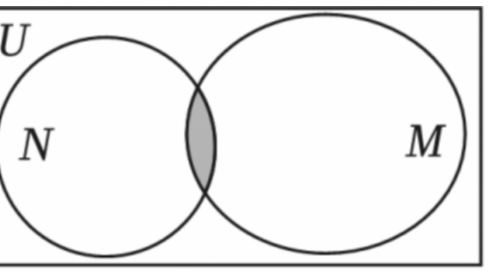
\includegraphics[width=0.30\textwidth]{figures/gao87_q14_venn.png}
\end{center}

\keepwithprev
A. $3$ 个\qquad B. $2$ 个\qquad C. $1$ 个\qquad D. 无穷多个

\ifanswer
\solbegin
\step{阴影部分所示的集合为 $M\cap N$，}
\step{$M=\{x\mid-1\leqslant x\leqslant3\}$，在此范围内的奇数有 $1$ 和 $3$，}
\step{所以集合 $M\cap N=\{1,3\}$ 共有 $2$ 个元素，故选 $B$.}
\solend
\fi

\item 已知实数 $a,b,c$ 满足 $a>b$，则下列不等式成立的是\mbox{（\quad）}

\keepwithprev
A. $-\dfrac1a<\dfrac1b$\qquad B. $a^2>b^2$\qquad C. $a\lvert c\rvert>b\lvert c\rvert$\qquad D. $\dfrac a{c^2+1}>\dfrac b{c^2+1}$

\ifanswer
\solbegin
\step{若 $a=1,b=-1$，则 $-1=-\dfrac1a=\dfrac1b=1$，$a^2=b^2=1$，则 AB 错误；}
\step{若 $a>b,c=0$，则 $a\lvert c\rvert=b\lvert c\rvert=0$，则 C 错误；}
\step{因为 $c^2+1\geqslant1$，所以 $0<\dfrac1{c^2+1}\leqslant1$，又 $a>b$，所以 $\dfrac a{c^2+1}>\dfrac b{c^2+1}$，}
\step{则 D 正确.}
\step{故选 $D$.}
\solend
\fi

\item 设集合 $P_1=\{x\mid x^2+ax+1>0\}$，$P_2=\{x\mid x^2+ax+2>0\}$，$Q_1=\{x\mid x^2+x+b>0\}$，
$Q_2=\{x\mid x^2+2x+b>0\}$，其中 $a$、$b\in\R$，下列说法中正确的是\mbox{（\quad）}

\keepwithprev
A. 对任意 $a$，$P_1$ 是 $P_2$ 的子集，对任意 $b$，$Q_1$ 不是 $Q_2$ 的子集

B. 对任意 $a$，$P_1$ 是 $P_2$ 的子集，存在 $b$，使得 $Q_1$ 是 $Q_2$ 的子集

C. 存在 $a$，使得 $P_1$ 不是 $P_2$ 的子集，对任意 $b$，$Q_1$ 不是 $Q_2$ 的子集

D. 存在 $a$，使得 $P_1$ 不是 $P_2$ 的子集，存在 $b$，使得 $Q_1$ 是 $Q_2$ 的子集

\ifanswer
\solbegin
\step{对于集合 $P_1=\{x\mid x^2+ax+1>0\}$，$P_2=\{x\mid x^2+ax+2>0\}$，}
\step{得当 $m\in P_1$ 时，即 $m^2+am+1>0$，得 $m^2+am+2>0$，}
\step{即有 $m\in P_2$，得对任意 $a$，$P_1$ 是 $P_2$ 的子集，}
\step{对于集合 $Q_1=\{x\mid x^2+x+b>0\}$，$Q_2=\{x\mid x^2+2x+b>0\}$，}
\step{当 $b=6$ 时，$Q_1=\{x\mid x^2+x+6>0\}=\R$，$Q_2=\{x\mid x^2+2x+6>0\}=\R$，}
\step{得 $Q_1$ 是 $Q_2$ 的子集，}
\step{当 $b=1$ 时，$Q_1=\{x\mid x^2+x+1>0\}=\R$，}
\step{$Q_2=\{x\mid x^2+2x+1>0\}=\{x\mid x\neq-1\}$，得 $Q_1$ 不是 $Q_2$ 的子集，}
\step{所以存在 $b$，使得 $Q_1$ 是 $Q_2$ 的子集，故选 $B$.}
\solend
\fi

\end{enumerate}

\bigsec{三、解答题}

\begin{enumerate}
\setcounter{enumi}{16}

\item 设 $m$ 为实数，求关于 $x$ 与 $y$ 的二元一次方程组 $\begin{cases}y=x+m\\ mx-y=4\end{cases}$ 的解集.

\ansspace*[8]

\ifanswer
\solbegin
\step{消去 $y$ 得 $(m-1)x=m+4$，}
\step{当 $m-1=0$，即 $m=1$ 时，$0=5$ 不成立，则 $x$ 无解，原方程组的解集为 $\varnothing$；}
\step{当 $m-1\neq0$，即 $m\neq1$ 时，则 $x=\dfrac{m+4}{m-1}$，$y=\dfrac{m+4}{m-1}+m=\dfrac{m^2+4}{m-1}$，}
\step{原方程组的解集为 $\left\{\left(\dfrac{m+4}{m-1},\dfrac{m^2+4}{m-1}\right)\right\}$.}
\step{综上所述，当 $m=1$ 时，方程组的解集为 $\varnothing$；}
\step{当 $m\neq1$ 时，方程组的解集为 $\left\{\left(\dfrac{m+4}{m-1},\dfrac{m^2+4}{m-1}\right)\right\}$.}
\solend
\fi

\item 设 $x<y<0$，试比较 $(x^2+y^2)(x-y)$ 与 $(x^2-y^2)(x+y)$ 的大小.

\ansspace*[9]

\ifanswer
\solbegin
\step{$(x^2+y^2)(x-y)-(x^2-y^2)(x+y)=(x-y)[x^2+y^2-(x+y)^2]=-2xy(x-y)$，}
\step{因为 $x<y<0$，所以 $xy>0$，$x-y<0$，所以 $-2xy(x-y)>0$，}
\step{即 $(x^2+y^2)(x-y)>(x^2-y^2)(x+y)$.}
\solend
\fi

\item 已知全集 $U=\R$，集合 $A=\left\{x\left|\dfrac{2+x}{3-x}>0\right.\right\}$，集合 $B=\{x\mid\lvert x-2\rvert>3\}$.

（1）求 $A\cup B$、$\overline A\cap B$.

（2）若集合 $C=\{x\mid x\leqslant a\}$，且 $A\cap C=A$，求实数 $a$ 的范围.

\ansspace*[10]

\ifanswer
\solbegin
\stepm{（1）}{由 $\lvert x-2\rvert>3$ 得 $x-2>3$ 或 $x-2<-3$，即 $x<-1$ 或 $x>5$，}
\step{所以 $B=(-\infty,-1)\cup(5,+\infty)$，}
\step{$A=\left\{x\left|\dfrac{2+x}{3-x}>0\right.\right\}=\{x\mid(2+x)(3-x)>0\}=(-2,3)$，}
\step{所以 $A\cup b=(-\infty,3)\cup(5m+\infty)$，}
\step{$\overline A=(-\infty,-2]\cup[3,+\infty)$，$\overline A\cap B=(-\infty,-2]\cup(5,+\infty)$.}
\stepm{（2）}{因为 $A\cap C=A$，所以 $A\subseteq C$，}
\step{因为 $A=(-2,3)$，所以实数 $a$ 的取值范围为 $\{a\mid a\geqslant3\}$.}
\solend
\fi

\item 已知函数 $f(x)=ax^2+4x+b\,(a<0,a,b\in\R)$，设关于 $x$ 的方程 $f(x)=0$ 的两实根为 $x_1$、
$x_2$，方程 $f(x)=x$ 的两实根为 $\alpha,\beta$.

（1）不等式 $f(x)<0$ 的解集是 $(-\infty,-3)\cup(5,+\infty)$，求不等式 $bx^2-ax-4<0$ 的解集；

（2）若 $a,b$ 均为负整数，且 $\lvert\alpha-\beta\rvert=1$，求 $f(x)$ 的解析式.

\ansspace*[12]

\ifanswer
\solbegin
\stepm{（1）}{$ax^2+4x+b<0$ 的解集为 $(-\infty,-3)\cup(5,+\infty)$，}
\step{所以 $-3,5$ 是方程 $ax^2+4x+b=0$ 的两根，所以 $\begin{cases}-3+5=-\dfrac4a\\ -3\times5=\dfrac ba\end{cases}\Rightarrow\begin{cases}a=-2\\ b=30\end{cases}$，}
\step{所以 $bx^2-ax-4<0$ 为 $30x^2+2x-4<0\Rightarrow15x^2+x-2<0$，}
\step{所以 $(3x-1)(5x+2)<0\Rightarrow-\dfrac25<x<\dfrac13$，}
\step{所以所求不等式的解集为 $\left\{x\left|-\dfrac25<x<\dfrac13\right.\right\}$.}
\stepm{（2）}{由题意得 $f(x)=ax^2+4x+b\,(a<0,a,b\in\R)$ 有两个不等实根为 $\alpha$、$\beta$，}
\step{所以 $\Delta=9-4ab>0$，$\alpha+\beta=-\dfrac3a$，$\alpha\beta=\dfrac ba$.}
\step{由 $\lvert\alpha-\beta\rvert=1$ 得 $(\alpha-\beta)^2=1$，即 $(\alpha+\beta)^2-4\alpha\beta=\dfrac9{a^2}-\dfrac{4b}a=1$，}
\step{所以 $9-4ab=a^2$，即 $a^2+4ab=9\,(a<0,a,b\in\R)$.}
\step{因为 $a,b$ 均为负整数，}
\step{所以 $\begin{cases}a=-1\\ a+4b=-9\end{cases}$ 或 $\begin{cases}a=-9\\ a+4b=-1\end{cases}$ 或 $\begin{cases}a=-3\\ a+4b=-3\end{cases}$，}
\step{显然后两种情况不合题意，应舍去，从而有 $\begin{cases}a=-1\\ a+4b=-9\end{cases}$，解得 $a=-1$，$b=-2$.}
\step{故所求函数解析式为 $f(x)=-x^2+4x-2$.}
\solend
\fi

\item 已知集合 $A=\{x\mid x=m^2+n^2,m\in\Z,n\in\Z\}$.

（1）判断 $2,5,25$ 是否属于集合 $A$；

（2）若正整数 $y$ 能表示为某个整数的平方，$z\in A$，证明：$yz\in A$；

（3）若集合 $B=\{x\mid x=4k+3,k\in\Z\}$，证明：$A\cap B=\varnothing$.

\ansspace*[14]

\ifanswer
\solbegin
\stepm{（1）}{由 $2=1^2+1^2$，$5=1^2+2^2$，$25=3^2+4^2$ 得 $2,5,25$ 属于集合 $A$；}
\stepm{（2）}{设 $y=a^2\,(a\in\Z)$，由 $z\in A$，设 $z=b^2+c^2\,(b\in\Z,c\in\Z)$，}
\step{则 $yz=a^2(b^2+c^2)=(ab)^2+(ac)^2$，}
\step{因为 $a\in\Z$，$b\in\Z$，$c\in\Z$，所以 $ab\in\Z$，$ac\in\Z$，所以 $yz\in A$；}
\stepm{（3）}{①当 $m$、$n$ 都为偶数时，设 $m=2k_1\,(k_1\in\Z)$，$n=2k_2\,(k_2\in\Z)$，}
\step{则 $x=m^2+n^2=4k_1^2+4k_2^2=4(k_1^2+k_2^2)$，此时 $x$ 为 $4$ 的倍数，}
\step{因为偶数 $\notin B$，所以 $A\cap B=\varnothing$；}
\step{②当 $m$、$n$ 都为奇数时，设 $m=2k_1+1\,(k_1\in\Z)$，$n=2k_2+1\,(k_2\in\Z)$，}
\step{则 $x=m^2+n^2=(2k_1+1)^2+(2k_2+1)^2=4(k_1^2+k_2^2+k_1+k_2)+2$，}
\step{此时 $x$ 为 $2$ 的倍数，因为偶数 $\notin B$，所以 $A\cap B=\varnothing$；}
\step{③当 $m$、$n$ 一奇一偶时，设 $m=2k_1+1\,(k_1\in\Z)$，$n=2k_2\,(k_2\in\Z)$，}
\step{则 $x=m^2+n^2=(2k_1+1)^2+(2k_2)^2=4(k_1^2+k_2^2+k_1)+1$，}
\step{此时 $x$ 被 $4$ 除余 $1$，而 $B$ 中元素被 $4$ 除余 $3$，此时 $A\cap B=\varnothing$.}
\step{综上，$A\cap B=\varnothing$.}
\solend
\fi

\end{enumerate}

\end{document}
"
%
% 原始材料：微信公众号“魔都数学加油站”文章，连载“27学年高一87”；
% 原文标题“27学年高一87——2026-2027年上海市五十四中学高一上10月月考”；
% 原文链接：https://mp.weixin.qq.com/s/pqPpSGQt0AhydcpaB8uEkQ。
% 页面标注发布时间 2026-10-27 17:43（上海）。
% 正文为 7 张 PNG 页（`原图/高一87_五十四中学_10月月考/01..07.png`），
% 尺寸混排（第 1、2 页为 4762×6735，第 3—7 页为 2560×3620），均按页序读取。
%
% 篇幅与题号：原卷自第 3 题起编号（第 1、2 题不在原文内）。填空题 3—12（10 题）、
% 选择题 13—16（4 题）、解答题 17—21（5 题），共 19 题。
%
% 讲评版：第 3、5、6 题只印【答案】（“$x\leqslant1$ 且 $y\leqslant1$”“$\{(2,6),(6,2)\}$”
% “$(-1,3]$”），本稿只给 \ans{}；其余 16 题印【解析】，其中选择题答案在解析末句
% “故选 A／B／D／B”。第 14 题题干带一幅韦恩图（裁自第 3 页原图、去粉色水印后转灰度），
% 三版都出。
%
% 副标题：原卷未印副标题。本稿按内容标作“集合与常用逻辑用语、不等式”。
%
% 原卷笔误/存疑（均照录未改，正文对应处另有 % 注）：
%   ① 第 19 题 (1) 解析作“所以 $A\cup b=(-\infty,3)\cup(5m+\infty)$”，两处均系排印错：
%      按上下文应为“$A\cup B=(-\infty,3)\cup(5,+\infty)$”（同页下一行 $\overline A\cap B$
%      的端点 $5$、$+\infty$ 也印证这一点）。原卷印作 $b$ 与 $5m+\infty$，照录未改。
%
% 与原卷的排版差异：
%   ① 原卷每题下直接印【答案】/【解析】，本稿按全稿惯例将答案与解析置于答案版；
%   ② 原卷未印副标题，本稿补出；填空横线统一排 \blankline[4.4em]；
%   ③ 原卷数集记号排斜体 $R$、$Z$、$N$，本稿按全稿惯例改用 $\R$、$\Z$、$\N$；
%   ④ 第 17—21 题的子问用行内“（1）（2）（3）”段，解析中的子问标号用 \stepm；
%   ⑤ 解答题按惯例加 \ansspace；选择题括号排 \mbox{（\quad）}。
%
% 行数核对：逐题数 \step/\stepm 条数，合计 86 条（Q4：1；Q7：4；Q8：2；Q9：2；Q10：3；
% Q11：9；Q12：3；Q13：2；Q14：3；Q15：5；Q16：9；Q17：6；Q18：3；Q19：7；Q20：13；
% Q21：14）；第 3、5、6 题只印【答案】，提 \ans{}，不计入 \step 账。原卷解析的换行
% 按语意合并，未逐行强拆。
%
\documentclass[a4paper,11pt]{article}
\usepackage{common}

\begin{document}

\examtitlest[7]{2026--2027 年五十四中学高一上 10 月月考}{集合与常用逻辑用语、不等式}

\bigsec{一、填空题}

\begin{enumerate}
\setcounter{enumi}{2}

\item “$x>1$ 或 $y>1$”的否定形式为\blankline[4.4em].

\ifanswer
\ans{$x\leqslant1$ 且 $y\leqslant1$}
\fi

\item 已知 $1<a<2$，$-3<b<3$，则 $a+b$ 的取值范围是\blankline[4.4em].

\ifanswer
\solbegin
\step{由不等式的可加性得 $-2<a+b<5$，故 $a+b$ 的取值范围是 $(-2,5)$.}
\solend
\fi

\item 方程组 $\begin{cases}x+y=8\\ xy=12\end{cases}$ 的解集为\blankline[4.4em].

\ifanswer
\ans{$\{(2,6),(6,2)\}$}
\fi

\item 不等式 $\dfrac{x-3}{x+1}\leqslant0$ 解集为\blankline[4.4em].

\ifanswer
\ans{$(-1,3]$}
\fi

\item 已知集合 $A=\{x\mid y=\sqrt{x+1}\}$，$B=\{y\mid y=x^2+5\}$，则 $A\cup B=\blankline[4.4em]$.

\ifanswer
\solbegin
\step{对于函数 $y=\sqrt{x+1}$，则 $x+1\geqslant0$，解得 $x\geqslant-1$，}
\step{所以 $A=\{x\mid y=\sqrt{x+1}\}=\{x\mid x\geqslant-1\}$，}
\step{因为 $x^2\geqslant0$，所以 $y=x^2+5\geqslant5$，所以 $B=\{y\mid y=x^2+5\}=\{y\mid y\geqslant5\}$，}
\step{所以 $A\cup B=\{x\mid x\geqslant-1\}$.}
\solend
\fi

\item 已知关于 $x$ 的不等式 $\lvert x+a\rvert<b$ 的解集为 $\{x\mid2<x<4\}$，则 $a+b$ 的值是\blankline[4.4em].

\ifanswer
\solbegin
\step{由 $\lvert x+a\rvert<b$，得 $-b-a<x<b-a$，则 $\begin{cases}-b-a=2\\ b-a=4\end{cases}$，解得 $a=-3$，$b=1$，}
\step{所以 $a+b=-2$.}
\solend
\fi

\item 已知一元二次方程 $x^2-2mx+m-1=0$ 的两实根为 $x_1,x_2$，且 $x_1^2+x_2^2=4$，则实数 $m$ 的值
是\blankline[4.4em].

\ifanswer
\solbegin
\step{由题意得 $x_1+x_2=2m$，$x_1x_2=m-1$，}
\step{所以 $x_1^2+x_2^2=(x_1+x_2)^2-2x_1x_2=4m^2-2m+2=4$，解得 $m=1$ 或 $m=-\dfrac12$.}
\solend
\fi

\item 已知集合 $A=\{x\mid x^2-x-6=0\}$，$B=\{y\mid ay-1=0\}$，若 $A\cap B=B$，则实数
$a=\blankline[4.4em]$.

\ifanswer
\solbegin
\step{$A=\{-2,3\}$，由 $A\cap B=B$，得 $B\subseteq A$，而 $B=\{y\mid ay-1=0\}$，}
\step{则当 $B=\varnothing$ 时，$a=0$；当 $B=\{-2\}$ 时，$-2a-1=0$，解得 $a=-\dfrac12$；}
\step{当 $B=\{3\}$ 时，$3a-1=0$，解得 $a=\dfrac13$，所以实数 $a$ 的值为 $-\dfrac12$ 或 $0$ 或 $\dfrac13$.}
\solend
\fi

\item 已知集合 $A=\{x\mid(m-1)x^2+(m-1)x+2\leqslant0,x\in\R\}$，$B=\left\{x\left|\dfrac{2x-1}{x^2+x+1}>1,x\in\R\right.\right\}$，
且 $A\cap B=A$，则实数 $m$ 的取值范围是\blankline[4.4em].

\ifanswer
\solbegin
\step{因为 $\dfrac{2x-1}{x^2+x+1}>1$，所以 $x^2-x+2<0$，显然不等式无解，}
\step{所以 $B=\left\{x\left|\dfrac{2x-1}{x^2+x+1}>1,x\in\R\right.\right\}=\varnothing$，而 $A\cap B=A$，则 $A=\varnothing$，}
\step{①当 $m=1$ 时，$2\leqslant0$ 不成立，此时 $A=\varnothing$，}
\step{②当 $m<1$ 时，$m-1<0$，函数 $y=(m-1)x^2+(m-1)x+2$，开口向下，}
\step{不等式 $(m-1)x^2+(m-1)x+2\leqslant0$ 有解，$A\neq\varnothing$，}
\step{③当 $m>1$ 时，函数 $y=(m-1)x^2+(m-1)x+2$，开口向上，}
\step{若不等式 $(m-1)x^2+(m-1)x+2\leqslant0$ 无解，}
\step{只需 $\Delta=(m-1)^2-8(m-1)<0$，解得 $1<m<9$，}
\step{综上，$m$ 的取值范围是 $[1,9]$.}
\solend
\fi

\item 设 $A$ 是整数集的一个非空子集，对于 $k\in A$，如果 $k-1\notin A$ 且 $k+1\notin A$，那么 $k$ 是 $A$
的一个“孤立元”. 给定 $S=\{1,2,3,4,5,6,7,8\}$，由 $S$ 的 $3$ 个元素构成的所有集合中，不含
“孤立元”的集合共有\blankline[3.6em]个.

\ifanswer
\solbegin
\step{由题意得，“孤立元”即为在集合中无与之相邻的元素，}
\step{满足条件的集合有 $\{1,2,3\},\{2,3,4\},\{3,4,5\},\{4,5,6\},\{5,6,7\},\{6,7,8\}$，}
\step{共 $6$ 个集合.}
\solend
\fi

\end{enumerate}

\bigsec{二、选择题}

\begin{enumerate}
\setcounter{enumi}{12}

\item “$m=2$”是“$m^2=4$”的\mbox{（\quad）}条件.

\keepwithprev
A. 充分非必要条件\qquad B. 必要非充分条件

C. 充要条件\qquad D. 既非充分又非必要条件

\ifanswer
\solbegin
\step{由 $m^2=4$，解得 $m=\pm2$，故“$m=2$”是“$m^2=4$”的充分不必要条件，}
\step{故选 $A$.}
\solend
\fi

\item 已知全集 $U=\R$，集合 $M=\{x\mid\lvert x-1\rvert\leqslant2\}$ 和 $N=\{x\mid x=2k-1,k\in\Z\}$ 的关系
的韦恩（$Venn$）图如图所示，则阴影部分所示的集合的元素共有\mbox{（\quad）}

\begin{center}
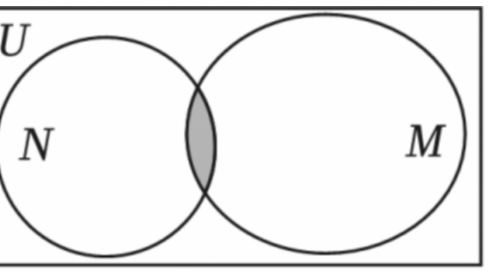
\includegraphics[width=0.30\textwidth]{figures/gao87_q14_venn.png}
\end{center}

\keepwithprev
A. $3$ 个\qquad B. $2$ 个\qquad C. $1$ 个\qquad D. 无穷多个

\ifanswer
\solbegin
\step{阴影部分所示的集合为 $M\cap N$，}
\step{$M=\{x\mid-1\leqslant x\leqslant3\}$，在此范围内的奇数有 $1$ 和 $3$，}
\step{所以集合 $M\cap N=\{1,3\}$ 共有 $2$ 个元素，故选 $B$.}
\solend
\fi

\item 已知实数 $a,b,c$ 满足 $a>b$，则下列不等式成立的是\mbox{（\quad）}

\keepwithprev
A. $-\dfrac1a<\dfrac1b$\qquad B. $a^2>b^2$\qquad C. $a\lvert c\rvert>b\lvert c\rvert$\qquad D. $\dfrac a{c^2+1}>\dfrac b{c^2+1}$

\ifanswer
\solbegin
\step{若 $a=1,b=-1$，则 $-1=-\dfrac1a=\dfrac1b=1$，$a^2=b^2=1$，则 AB 错误；}
\step{若 $a>b,c=0$，则 $a\lvert c\rvert=b\lvert c\rvert=0$，则 C 错误；}
\step{因为 $c^2+1\geqslant1$，所以 $0<\dfrac1{c^2+1}\leqslant1$，又 $a>b$，所以 $\dfrac a{c^2+1}>\dfrac b{c^2+1}$，}
\step{则 D 正确.}
\step{故选 $D$.}
\solend
\fi

\item 设集合 $P_1=\{x\mid x^2+ax+1>0\}$，$P_2=\{x\mid x^2+ax+2>0\}$，$Q_1=\{x\mid x^2+x+b>0\}$，
$Q_2=\{x\mid x^2+2x+b>0\}$，其中 $a$、$b\in\R$，下列说法中正确的是\mbox{（\quad）}

\keepwithprev
A. 对任意 $a$，$P_1$ 是 $P_2$ 的子集，对任意 $b$，$Q_1$ 不是 $Q_2$ 的子集

B. 对任意 $a$，$P_1$ 是 $P_2$ 的子集，存在 $b$，使得 $Q_1$ 是 $Q_2$ 的子集

C. 存在 $a$，使得 $P_1$ 不是 $P_2$ 的子集，对任意 $b$，$Q_1$ 不是 $Q_2$ 的子集

D. 存在 $a$，使得 $P_1$ 不是 $P_2$ 的子集，存在 $b$，使得 $Q_1$ 是 $Q_2$ 的子集

\ifanswer
\solbegin
\step{对于集合 $P_1=\{x\mid x^2+ax+1>0\}$，$P_2=\{x\mid x^2+ax+2>0\}$，}
\step{得当 $m\in P_1$ 时，即 $m^2+am+1>0$，得 $m^2+am+2>0$，}
\step{即有 $m\in P_2$，得对任意 $a$，$P_1$ 是 $P_2$ 的子集，}
\step{对于集合 $Q_1=\{x\mid x^2+x+b>0\}$，$Q_2=\{x\mid x^2+2x+b>0\}$，}
\step{当 $b=6$ 时，$Q_1=\{x\mid x^2+x+6>0\}=\R$，$Q_2=\{x\mid x^2+2x+6>0\}=\R$，}
\step{得 $Q_1$ 是 $Q_2$ 的子集，}
\step{当 $b=1$ 时，$Q_1=\{x\mid x^2+x+1>0\}=\R$，}
\step{$Q_2=\{x\mid x^2+2x+1>0\}=\{x\mid x\neq-1\}$，得 $Q_1$ 不是 $Q_2$ 的子集，}
\step{所以存在 $b$，使得 $Q_1$ 是 $Q_2$ 的子集，故选 $B$.}
\solend
\fi

\end{enumerate}

\bigsec{三、解答题}

\begin{enumerate}
\setcounter{enumi}{16}

\item 设 $m$ 为实数，求关于 $x$ 与 $y$ 的二元一次方程组 $\begin{cases}y=x+m\\ mx-y=4\end{cases}$ 的解集.

\ansspace*[8]

\ifanswer
\solbegin
\step{消去 $y$ 得 $(m-1)x=m+4$，}
\step{当 $m-1=0$，即 $m=1$ 时，$0=5$ 不成立，则 $x$ 无解，原方程组的解集为 $\varnothing$；}
\step{当 $m-1\neq0$，即 $m\neq1$ 时，则 $x=\dfrac{m+4}{m-1}$，$y=\dfrac{m+4}{m-1}+m=\dfrac{m^2+4}{m-1}$，}
\step{原方程组的解集为 $\left\{\left(\dfrac{m+4}{m-1},\dfrac{m^2+4}{m-1}\right)\right\}$.}
\step{综上所述，当 $m=1$ 时，方程组的解集为 $\varnothing$；}
\step{当 $m\neq1$ 时，方程组的解集为 $\left\{\left(\dfrac{m+4}{m-1},\dfrac{m^2+4}{m-1}\right)\right\}$.}
\solend
\fi

\item 设 $x<y<0$，试比较 $(x^2+y^2)(x-y)$ 与 $(x^2-y^2)(x+y)$ 的大小.

\ansspace*[9]

\ifanswer
\solbegin
\step{$(x^2+y^2)(x-y)-(x^2-y^2)(x+y)=(x-y)[x^2+y^2-(x+y)^2]=-2xy(x-y)$，}
\step{因为 $x<y<0$，所以 $xy>0$，$x-y<0$，所以 $-2xy(x-y)>0$，}
\step{即 $(x^2+y^2)(x-y)>(x^2-y^2)(x+y)$.}
\solend
\fi

\item 已知全集 $U=\R$，集合 $A=\left\{x\left|\dfrac{2+x}{3-x}>0\right.\right\}$，集合 $B=\{x\mid\lvert x-2\rvert>3\}$.

（1）求 $A\cup B$、$\overline A\cap B$.

（2）若集合 $C=\{x\mid x\leqslant a\}$，且 $A\cap C=A$，求实数 $a$ 的范围.

\ansspace*[10]

\ifanswer
\solbegin
\stepm{（1）}{由 $\lvert x-2\rvert>3$ 得 $x-2>3$ 或 $x-2<-3$，即 $x<-1$ 或 $x>5$，}
\step{所以 $B=(-\infty,-1)\cup(5,+\infty)$，}
\step{$A=\left\{x\left|\dfrac{2+x}{3-x}>0\right.\right\}=\{x\mid(2+x)(3-x)>0\}=(-2,3)$，}
\step{所以 $A\cup b=(-\infty,3)\cup(5m+\infty)$，}
\step{$\overline A=(-\infty,-2]\cup[3,+\infty)$，$\overline A\cap B=(-\infty,-2]\cup(5,+\infty)$.}
\stepm{（2）}{因为 $A\cap C=A$，所以 $A\subseteq C$，}
\step{因为 $A=(-2,3)$，所以实数 $a$ 的取值范围为 $\{a\mid a\geqslant3\}$.}
\solend
\fi

\item 已知函数 $f(x)=ax^2+4x+b\,(a<0,a,b\in\R)$，设关于 $x$ 的方程 $f(x)=0$ 的两实根为 $x_1$、
$x_2$，方程 $f(x)=x$ 的两实根为 $\alpha,\beta$.

（1）不等式 $f(x)<0$ 的解集是 $(-\infty,-3)\cup(5,+\infty)$，求不等式 $bx^2-ax-4<0$ 的解集；

（2）若 $a,b$ 均为负整数，且 $\lvert\alpha-\beta\rvert=1$，求 $f(x)$ 的解析式.

\ansspace*[12]

\ifanswer
\solbegin
\stepm{（1）}{$ax^2+4x+b<0$ 的解集为 $(-\infty,-3)\cup(5,+\infty)$，}
\step{所以 $-3,5$ 是方程 $ax^2+4x+b=0$ 的两根，所以 $\begin{cases}-3+5=-\dfrac4a\\ -3\times5=\dfrac ba\end{cases}\Rightarrow\begin{cases}a=-2\\ b=30\end{cases}$，}
\step{所以 $bx^2-ax-4<0$ 为 $30x^2+2x-4<0\Rightarrow15x^2+x-2<0$，}
\step{所以 $(3x-1)(5x+2)<0\Rightarrow-\dfrac25<x<\dfrac13$，}
\step{所以所求不等式的解集为 $\left\{x\left|-\dfrac25<x<\dfrac13\right.\right\}$.}
\stepm{（2）}{由题意得 $f(x)=ax^2+4x+b\,(a<0,a,b\in\R)$ 有两个不等实根为 $\alpha$、$\beta$，}
\step{所以 $\Delta=9-4ab>0$，$\alpha+\beta=-\dfrac3a$，$\alpha\beta=\dfrac ba$.}
\step{由 $\lvert\alpha-\beta\rvert=1$ 得 $(\alpha-\beta)^2=1$，即 $(\alpha+\beta)^2-4\alpha\beta=\dfrac9{a^2}-\dfrac{4b}a=1$，}
\step{所以 $9-4ab=a^2$，即 $a^2+4ab=9\,(a<0,a,b\in\R)$.}
\step{因为 $a,b$ 均为负整数，}
\step{所以 $\begin{cases}a=-1\\ a+4b=-9\end{cases}$ 或 $\begin{cases}a=-9\\ a+4b=-1\end{cases}$ 或 $\begin{cases}a=-3\\ a+4b=-3\end{cases}$，}
\step{显然后两种情况不合题意，应舍去，从而有 $\begin{cases}a=-1\\ a+4b=-9\end{cases}$，解得 $a=-1$，$b=-2$.}
\step{故所求函数解析式为 $f(x)=-x^2+4x-2$.}
\solend
\fi

\item 已知集合 $A=\{x\mid x=m^2+n^2,m\in\Z,n\in\Z\}$.

（1）判断 $2,5,25$ 是否属于集合 $A$；

（2）若正整数 $y$ 能表示为某个整数的平方，$z\in A$，证明：$yz\in A$；

（3）若集合 $B=\{x\mid x=4k+3,k\in\Z\}$，证明：$A\cap B=\varnothing$.

\ansspace*[14]

\ifanswer
\solbegin
\stepm{（1）}{由 $2=1^2+1^2$，$5=1^2+2^2$，$25=3^2+4^2$ 得 $2,5,25$ 属于集合 $A$；}
\stepm{（2）}{设 $y=a^2\,(a\in\Z)$，由 $z\in A$，设 $z=b^2+c^2\,(b\in\Z,c\in\Z)$，}
\step{则 $yz=a^2(b^2+c^2)=(ab)^2+(ac)^2$，}
\step{因为 $a\in\Z$，$b\in\Z$，$c\in\Z$，所以 $ab\in\Z$，$ac\in\Z$，所以 $yz\in A$；}
\stepm{（3）}{①当 $m$、$n$ 都为偶数时，设 $m=2k_1\,(k_1\in\Z)$，$n=2k_2\,(k_2\in\Z)$，}
\step{则 $x=m^2+n^2=4k_1^2+4k_2^2=4(k_1^2+k_2^2)$，此时 $x$ 为 $4$ 的倍数，}
\step{因为偶数 $\notin B$，所以 $A\cap B=\varnothing$；}
\step{②当 $m$、$n$ 都为奇数时，设 $m=2k_1+1\,(k_1\in\Z)$，$n=2k_2+1\,(k_2\in\Z)$，}
\step{则 $x=m^2+n^2=(2k_1+1)^2+(2k_2+1)^2=4(k_1^2+k_2^2+k_1+k_2)+2$，}
\step{此时 $x$ 为 $2$ 的倍数，因为偶数 $\notin B$，所以 $A\cap B=\varnothing$；}
\step{③当 $m$、$n$ 一奇一偶时，设 $m=2k_1+1\,(k_1\in\Z)$，$n=2k_2\,(k_2\in\Z)$，}
\step{则 $x=m^2+n^2=(2k_1+1)^2+(2k_2)^2=4(k_1^2+k_2^2+k_1)+1$，}
\step{此时 $x$ 被 $4$ 除余 $1$，而 $B$ 中元素被 $4$ 除余 $3$，此时 $A\cap B=\varnothing$.}
\step{综上，$A\cap B=\varnothing$.}
\solend
\fi

\end{enumerate}

\end{document}
"
%
% 原始材料：微信公众号“魔都数学加油站”文章，连载“27学年高一87”；
% 原文标题“27学年高一87——2026-2027年上海市五十四中学高一上10月月考”；
% 原文链接：https://mp.weixin.qq.com/s/pqPpSGQt0AhydcpaB8uEkQ。
% 页面标注发布时间 2026-10-27 17:43（上海）。
% 正文为 7 张 PNG 页（`原图/高一87_五十四中学_10月月考/01..07.png`），
% 尺寸混排（第 1、2 页为 4762×6735，第 3—7 页为 2560×3620），均按页序读取。
%
% 篇幅与题号：原卷自第 3 题起编号（第 1、2 题不在原文内）。填空题 3—12（10 题）、
% 选择题 13—16（4 题）、解答题 17—21（5 题），共 19 题。
%
% 讲评版：第 3、5、6 题只印【答案】（“$x\leqslant1$ 且 $y\leqslant1$”“$\{(2,6),(6,2)\}$”
% “$(-1,3]$”），本稿只给 \ans{}；其余 16 题印【解析】，其中选择题答案在解析末句
% “故选 A／B／D／B”。第 14 题题干带一幅韦恩图（裁自第 3 页原图、去粉色水印后转灰度），
% 三版都出。
%
% 副标题：原卷未印副标题。本稿按内容标作“集合与常用逻辑用语、不等式”。
%
% 原卷笔误/存疑（均照录未改，正文对应处另有 % 注）：
%   ① 第 19 题 (1) 解析作“所以 $A\cup b=(-\infty,3)\cup(5m+\infty)$”，两处均系排印错：
%      按上下文应为“$A\cup B=(-\infty,3)\cup(5,+\infty)$”（同页下一行 $\overline A\cap B$
%      的端点 $5$、$+\infty$ 也印证这一点）。原卷印作 $b$ 与 $5m+\infty$，照录未改。
%
% 与原卷的排版差异：
%   ① 原卷每题下直接印【答案】/【解析】，本稿按全稿惯例将答案与解析置于答案版；
%   ② 原卷未印副标题，本稿补出；填空横线统一排 \blankline[4.4em]；
%   ③ 原卷数集记号排斜体 $R$、$Z$、$N$，本稿按全稿惯例改用 $\R$、$\Z$、$\N$；
%   ④ 第 17—21 题的子问用行内“（1）（2）（3）”段，解析中的子问标号用 \stepm；
%   ⑤ 解答题按惯例加 \ansspace；选择题括号排 \mbox{（\quad）}。
%
% 行数核对：逐题数 \step/\stepm 条数，合计 86 条（Q4：1；Q7：4；Q8：2；Q9：2；Q10：3；
% Q11：9；Q12：3；Q13：2；Q14：3；Q15：5；Q16：9；Q17：6；Q18：3；Q19：7；Q20：13；
% Q21：14）；第 3、5、6 题只印【答案】，提 \ans{}，不计入 \step 账。原卷解析的换行
% 按语意合并，未逐行强拆。
%
\documentclass[a4paper,11pt]{article}
\usepackage{common}

\begin{document}

\examtitlest[7]{2026--2027 年五十四中学高一上 10 月月考}{集合与常用逻辑用语、不等式}

\bigsec{一、填空题}

\begin{enumerate}
\setcounter{enumi}{2}

\item “$x>1$ 或 $y>1$”的否定形式为\blankline[4.4em].

\ifanswer
\ans{$x\leqslant1$ 且 $y\leqslant1$}
\fi

\item 已知 $1<a<2$，$-3<b<3$，则 $a+b$ 的取值范围是\blankline[4.4em].

\ifanswer
\solbegin
\step{由不等式的可加性得 $-2<a+b<5$，故 $a+b$ 的取值范围是 $(-2,5)$.}
\solend
\fi

\item 方程组 $\begin{cases}x+y=8\\ xy=12\end{cases}$ 的解集为\blankline[4.4em].

\ifanswer
\ans{$\{(2,6),(6,2)\}$}
\fi

\item 不等式 $\dfrac{x-3}{x+1}\leqslant0$ 解集为\blankline[4.4em].

\ifanswer
\ans{$(-1,3]$}
\fi

\item 已知集合 $A=\{x\mid y=\sqrt{x+1}\}$，$B=\{y\mid y=x^2+5\}$，则 $A\cup B=\blankline[4.4em]$.

\ifanswer
\solbegin
\step{对于函数 $y=\sqrt{x+1}$，则 $x+1\geqslant0$，解得 $x\geqslant-1$，}
\step{所以 $A=\{x\mid y=\sqrt{x+1}\}=\{x\mid x\geqslant-1\}$，}
\step{因为 $x^2\geqslant0$，所以 $y=x^2+5\geqslant5$，所以 $B=\{y\mid y=x^2+5\}=\{y\mid y\geqslant5\}$，}
\step{所以 $A\cup B=\{x\mid x\geqslant-1\}$.}
\solend
\fi

\item 已知关于 $x$ 的不等式 $\lvert x+a\rvert<b$ 的解集为 $\{x\mid2<x<4\}$，则 $a+b$ 的值是\blankline[4.4em].

\ifanswer
\solbegin
\step{由 $\lvert x+a\rvert<b$，得 $-b-a<x<b-a$，则 $\begin{cases}-b-a=2\\ b-a=4\end{cases}$，解得 $a=-3$，$b=1$，}
\step{所以 $a+b=-2$.}
\solend
\fi

\item 已知一元二次方程 $x^2-2mx+m-1=0$ 的两实根为 $x_1,x_2$，且 $x_1^2+x_2^2=4$，则实数 $m$ 的值
是\blankline[4.4em].

\ifanswer
\solbegin
\step{由题意得 $x_1+x_2=2m$，$x_1x_2=m-1$，}
\step{所以 $x_1^2+x_2^2=(x_1+x_2)^2-2x_1x_2=4m^2-2m+2=4$，解得 $m=1$ 或 $m=-\dfrac12$.}
\solend
\fi

\item 已知集合 $A=\{x\mid x^2-x-6=0\}$，$B=\{y\mid ay-1=0\}$，若 $A\cap B=B$，则实数
$a=\blankline[4.4em]$.

\ifanswer
\solbegin
\step{$A=\{-2,3\}$，由 $A\cap B=B$，得 $B\subseteq A$，而 $B=\{y\mid ay-1=0\}$，}
\step{则当 $B=\varnothing$ 时，$a=0$；当 $B=\{-2\}$ 时，$-2a-1=0$，解得 $a=-\dfrac12$；}
\step{当 $B=\{3\}$ 时，$3a-1=0$，解得 $a=\dfrac13$，所以实数 $a$ 的值为 $-\dfrac12$ 或 $0$ 或 $\dfrac13$.}
\solend
\fi

\item 已知集合 $A=\{x\mid(m-1)x^2+(m-1)x+2\leqslant0,x\in\R\}$，$B=\left\{x\left|\dfrac{2x-1}{x^2+x+1}>1,x\in\R\right.\right\}$，
且 $A\cap B=A$，则实数 $m$ 的取值范围是\blankline[4.4em].

\ifanswer
\solbegin
\step{因为 $\dfrac{2x-1}{x^2+x+1}>1$，所以 $x^2-x+2<0$，显然不等式无解，}
\step{所以 $B=\left\{x\left|\dfrac{2x-1}{x^2+x+1}>1,x\in\R\right.\right\}=\varnothing$，而 $A\cap B=A$，则 $A=\varnothing$，}
\step{①当 $m=1$ 时，$2\leqslant0$ 不成立，此时 $A=\varnothing$，}
\step{②当 $m<1$ 时，$m-1<0$，函数 $y=(m-1)x^2+(m-1)x+2$，开口向下，}
\step{不等式 $(m-1)x^2+(m-1)x+2\leqslant0$ 有解，$A\neq\varnothing$，}
\step{③当 $m>1$ 时，函数 $y=(m-1)x^2+(m-1)x+2$，开口向上，}
\step{若不等式 $(m-1)x^2+(m-1)x+2\leqslant0$ 无解，}
\step{只需 $\Delta=(m-1)^2-8(m-1)<0$，解得 $1<m<9$，}
\step{综上，$m$ 的取值范围是 $[1,9]$.}
\solend
\fi

\item 设 $A$ 是整数集的一个非空子集，对于 $k\in A$，如果 $k-1\notin A$ 且 $k+1\notin A$，那么 $k$ 是 $A$
的一个“孤立元”. 给定 $S=\{1,2,3,4,5,6,7,8\}$，由 $S$ 的 $3$ 个元素构成的所有集合中，不含
“孤立元”的集合共有\blankline[3.6em]个.

\ifanswer
\solbegin
\step{由题意得，“孤立元”即为在集合中无与之相邻的元素，}
\step{满足条件的集合有 $\{1,2,3\},\{2,3,4\},\{3,4,5\},\{4,5,6\},\{5,6,7\},\{6,7,8\}$，}
\step{共 $6$ 个集合.}
\solend
\fi

\end{enumerate}

\bigsec{二、选择题}

\begin{enumerate}
\setcounter{enumi}{12}

\item “$m=2$”是“$m^2=4$”的\mbox{（\quad）}条件.

\keepwithprev
A. 充分非必要条件\qquad B. 必要非充分条件

C. 充要条件\qquad D. 既非充分又非必要条件

\ifanswer
\solbegin
\step{由 $m^2=4$，解得 $m=\pm2$，故“$m=2$”是“$m^2=4$”的充分不必要条件，}
\step{故选 $A$.}
\solend
\fi

\item 已知全集 $U=\R$，集合 $M=\{x\mid\lvert x-1\rvert\leqslant2\}$ 和 $N=\{x\mid x=2k-1,k\in\Z\}$ 的关系
的韦恩（$Venn$）图如图所示，则阴影部分所示的集合的元素共有\mbox{（\quad）}

\begin{center}
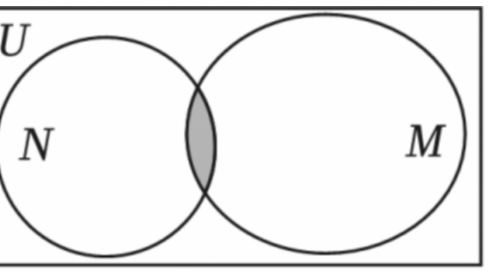
\includegraphics[width=0.30\textwidth]{figures/gao87_q14_venn.png}
\end{center}

\keepwithprev
A. $3$ 个\qquad B. $2$ 个\qquad C. $1$ 个\qquad D. 无穷多个

\ifanswer
\solbegin
\step{阴影部分所示的集合为 $M\cap N$，}
\step{$M=\{x\mid-1\leqslant x\leqslant3\}$，在此范围内的奇数有 $1$ 和 $3$，}
\step{所以集合 $M\cap N=\{1,3\}$ 共有 $2$ 个元素，故选 $B$.}
\solend
\fi

\item 已知实数 $a,b,c$ 满足 $a>b$，则下列不等式成立的是\mbox{（\quad）}

\keepwithprev
A. $-\dfrac1a<\dfrac1b$\qquad B. $a^2>b^2$\qquad C. $a\lvert c\rvert>b\lvert c\rvert$\qquad D. $\dfrac a{c^2+1}>\dfrac b{c^2+1}$

\ifanswer
\solbegin
\step{若 $a=1,b=-1$，则 $-1=-\dfrac1a=\dfrac1b=1$，$a^2=b^2=1$，则 AB 错误；}
\step{若 $a>b,c=0$，则 $a\lvert c\rvert=b\lvert c\rvert=0$，则 C 错误；}
\step{因为 $c^2+1\geqslant1$，所以 $0<\dfrac1{c^2+1}\leqslant1$，又 $a>b$，所以 $\dfrac a{c^2+1}>\dfrac b{c^2+1}$，}
\step{则 D 正确.}
\step{故选 $D$.}
\solend
\fi

\item 设集合 $P_1=\{x\mid x^2+ax+1>0\}$，$P_2=\{x\mid x^2+ax+2>0\}$，$Q_1=\{x\mid x^2+x+b>0\}$，
$Q_2=\{x\mid x^2+2x+b>0\}$，其中 $a$、$b\in\R$，下列说法中正确的是\mbox{（\quad）}

\keepwithprev
A. 对任意 $a$，$P_1$ 是 $P_2$ 的子集，对任意 $b$，$Q_1$ 不是 $Q_2$ 的子集

B. 对任意 $a$，$P_1$ 是 $P_2$ 的子集，存在 $b$，使得 $Q_1$ 是 $Q_2$ 的子集

C. 存在 $a$，使得 $P_1$ 不是 $P_2$ 的子集，对任意 $b$，$Q_1$ 不是 $Q_2$ 的子集

D. 存在 $a$，使得 $P_1$ 不是 $P_2$ 的子集，存在 $b$，使得 $Q_1$ 是 $Q_2$ 的子集

\ifanswer
\solbegin
\step{对于集合 $P_1=\{x\mid x^2+ax+1>0\}$，$P_2=\{x\mid x^2+ax+2>0\}$，}
\step{得当 $m\in P_1$ 时，即 $m^2+am+1>0$，得 $m^2+am+2>0$，}
\step{即有 $m\in P_2$，得对任意 $a$，$P_1$ 是 $P_2$ 的子集，}
\step{对于集合 $Q_1=\{x\mid x^2+x+b>0\}$，$Q_2=\{x\mid x^2+2x+b>0\}$，}
\step{当 $b=6$ 时，$Q_1=\{x\mid x^2+x+6>0\}=\R$，$Q_2=\{x\mid x^2+2x+6>0\}=\R$，}
\step{得 $Q_1$ 是 $Q_2$ 的子集，}
\step{当 $b=1$ 时，$Q_1=\{x\mid x^2+x+1>0\}=\R$，}
\step{$Q_2=\{x\mid x^2+2x+1>0\}=\{x\mid x\neq-1\}$，得 $Q_1$ 不是 $Q_2$ 的子集，}
\step{所以存在 $b$，使得 $Q_1$ 是 $Q_2$ 的子集，故选 $B$.}
\solend
\fi

\end{enumerate}

\bigsec{三、解答题}

\begin{enumerate}
\setcounter{enumi}{16}

\item 设 $m$ 为实数，求关于 $x$ 与 $y$ 的二元一次方程组 $\begin{cases}y=x+m\\ mx-y=4\end{cases}$ 的解集.

\ansspace*[8]

\ifanswer
\solbegin
\step{消去 $y$ 得 $(m-1)x=m+4$，}
\step{当 $m-1=0$，即 $m=1$ 时，$0=5$ 不成立，则 $x$ 无解，原方程组的解集为 $\varnothing$；}
\step{当 $m-1\neq0$，即 $m\neq1$ 时，则 $x=\dfrac{m+4}{m-1}$，$y=\dfrac{m+4}{m-1}+m=\dfrac{m^2+4}{m-1}$，}
\step{原方程组的解集为 $\left\{\left(\dfrac{m+4}{m-1},\dfrac{m^2+4}{m-1}\right)\right\}$.}
\step{综上所述，当 $m=1$ 时，方程组的解集为 $\varnothing$；}
\step{当 $m\neq1$ 时，方程组的解集为 $\left\{\left(\dfrac{m+4}{m-1},\dfrac{m^2+4}{m-1}\right)\right\}$.}
\solend
\fi

\item 设 $x<y<0$，试比较 $(x^2+y^2)(x-y)$ 与 $(x^2-y^2)(x+y)$ 的大小.

\ansspace*[9]

\ifanswer
\solbegin
\step{$(x^2+y^2)(x-y)-(x^2-y^2)(x+y)=(x-y)[x^2+y^2-(x+y)^2]=-2xy(x-y)$，}
\step{因为 $x<y<0$，所以 $xy>0$，$x-y<0$，所以 $-2xy(x-y)>0$，}
\step{即 $(x^2+y^2)(x-y)>(x^2-y^2)(x+y)$.}
\solend
\fi

\item 已知全集 $U=\R$，集合 $A=\left\{x\left|\dfrac{2+x}{3-x}>0\right.\right\}$，集合 $B=\{x\mid\lvert x-2\rvert>3\}$.

（1）求 $A\cup B$、$\overline A\cap B$.

（2）若集合 $C=\{x\mid x\leqslant a\}$，且 $A\cap C=A$，求实数 $a$ 的范围.

\ansspace*[10]

\ifanswer
\solbegin
\stepm{（1）}{由 $\lvert x-2\rvert>3$ 得 $x-2>3$ 或 $x-2<-3$，即 $x<-1$ 或 $x>5$，}
\step{所以 $B=(-\infty,-1)\cup(5,+\infty)$，}
\step{$A=\left\{x\left|\dfrac{2+x}{3-x}>0\right.\right\}=\{x\mid(2+x)(3-x)>0\}=(-2,3)$，}
\step{所以 $A\cup b=(-\infty,3)\cup(5m+\infty)$，}
\step{$\overline A=(-\infty,-2]\cup[3,+\infty)$，$\overline A\cap B=(-\infty,-2]\cup(5,+\infty)$.}
\stepm{（2）}{因为 $A\cap C=A$，所以 $A\subseteq C$，}
\step{因为 $A=(-2,3)$，所以实数 $a$ 的取值范围为 $\{a\mid a\geqslant3\}$.}
\solend
\fi

\item 已知函数 $f(x)=ax^2+4x+b\,(a<0,a,b\in\R)$，设关于 $x$ 的方程 $f(x)=0$ 的两实根为 $x_1$、
$x_2$，方程 $f(x)=x$ 的两实根为 $\alpha,\beta$.

（1）不等式 $f(x)<0$ 的解集是 $(-\infty,-3)\cup(5,+\infty)$，求不等式 $bx^2-ax-4<0$ 的解集；

（2）若 $a,b$ 均为负整数，且 $\lvert\alpha-\beta\rvert=1$，求 $f(x)$ 的解析式.

\ansspace*[12]

\ifanswer
\solbegin
\stepm{（1）}{$ax^2+4x+b<0$ 的解集为 $(-\infty,-3)\cup(5,+\infty)$，}
\step{所以 $-3,5$ 是方程 $ax^2+4x+b=0$ 的两根，所以 $\begin{cases}-3+5=-\dfrac4a\\ -3\times5=\dfrac ba\end{cases}\Rightarrow\begin{cases}a=-2\\ b=30\end{cases}$，}
\step{所以 $bx^2-ax-4<0$ 为 $30x^2+2x-4<0\Rightarrow15x^2+x-2<0$，}
\step{所以 $(3x-1)(5x+2)<0\Rightarrow-\dfrac25<x<\dfrac13$，}
\step{所以所求不等式的解集为 $\left\{x\left|-\dfrac25<x<\dfrac13\right.\right\}$.}
\stepm{（2）}{由题意得 $f(x)=ax^2+4x+b\,(a<0,a,b\in\R)$ 有两个不等实根为 $\alpha$、$\beta$，}
\step{所以 $\Delta=9-4ab>0$，$\alpha+\beta=-\dfrac3a$，$\alpha\beta=\dfrac ba$.}
\step{由 $\lvert\alpha-\beta\rvert=1$ 得 $(\alpha-\beta)^2=1$，即 $(\alpha+\beta)^2-4\alpha\beta=\dfrac9{a^2}-\dfrac{4b}a=1$，}
\step{所以 $9-4ab=a^2$，即 $a^2+4ab=9\,(a<0,a,b\in\R)$.}
\step{因为 $a,b$ 均为负整数，}
\step{所以 $\begin{cases}a=-1\\ a+4b=-9\end{cases}$ 或 $\begin{cases}a=-9\\ a+4b=-1\end{cases}$ 或 $\begin{cases}a=-3\\ a+4b=-3\end{cases}$，}
\step{显然后两种情况不合题意，应舍去，从而有 $\begin{cases}a=-1\\ a+4b=-9\end{cases}$，解得 $a=-1$，$b=-2$.}
\step{故所求函数解析式为 $f(x)=-x^2+4x-2$.}
\solend
\fi

\item 已知集合 $A=\{x\mid x=m^2+n^2,m\in\Z,n\in\Z\}$.

（1）判断 $2,5,25$ 是否属于集合 $A$；

（2）若正整数 $y$ 能表示为某个整数的平方，$z\in A$，证明：$yz\in A$；

（3）若集合 $B=\{x\mid x=4k+3,k\in\Z\}$，证明：$A\cap B=\varnothing$.

\ansspace*[14]

\ifanswer
\solbegin
\stepm{（1）}{由 $2=1^2+1^2$，$5=1^2+2^2$，$25=3^2+4^2$ 得 $2,5,25$ 属于集合 $A$；}
\stepm{（2）}{设 $y=a^2\,(a\in\Z)$，由 $z\in A$，设 $z=b^2+c^2\,(b\in\Z,c\in\Z)$，}
\step{则 $yz=a^2(b^2+c^2)=(ab)^2+(ac)^2$，}
\step{因为 $a\in\Z$，$b\in\Z$，$c\in\Z$，所以 $ab\in\Z$，$ac\in\Z$，所以 $yz\in A$；}
\stepm{（3）}{①当 $m$、$n$ 都为偶数时，设 $m=2k_1\,(k_1\in\Z)$，$n=2k_2\,(k_2\in\Z)$，}
\step{则 $x=m^2+n^2=4k_1^2+4k_2^2=4(k_1^2+k_2^2)$，此时 $x$ 为 $4$ 的倍数，}
\step{因为偶数 $\notin B$，所以 $A\cap B=\varnothing$；}
\step{②当 $m$、$n$ 都为奇数时，设 $m=2k_1+1\,(k_1\in\Z)$，$n=2k_2+1\,(k_2\in\Z)$，}
\step{则 $x=m^2+n^2=(2k_1+1)^2+(2k_2+1)^2=4(k_1^2+k_2^2+k_1+k_2)+2$，}
\step{此时 $x$ 为 $2$ 的倍数，因为偶数 $\notin B$，所以 $A\cap B=\varnothing$；}
\step{③当 $m$、$n$ 一奇一偶时，设 $m=2k_1+1\,(k_1\in\Z)$，$n=2k_2\,(k_2\in\Z)$，}
\step{则 $x=m^2+n^2=(2k_1+1)^2+(2k_2)^2=4(k_1^2+k_2^2+k_1)+1$，}
\step{此时 $x$ 被 $4$ 除余 $1$，而 $B$ 中元素被 $4$ 除余 $3$，此时 $A\cap B=\varnothing$.}
\step{综上，$A\cap B=\varnothing$.}
\solend
\fi

\end{enumerate}

\end{document}
